\documentclass[11pt,twocolumn]{article}

%\usepackage{sectsty}
\usepackage{titlesec}
\usepackage{url}

\usepackage{eso-pic}

\usepackage{setspace}
%\doublespacing
%\onehalfspacing


% line
\usepackage[object=vectorian]{pgfornament} %%  http://altermundus.com/pages/tkz/ornament/index.html

\definecolor{darkRed}{rgb}{.2,.0,.1}

\newcommand{\decoline}{%

\vspace{-2em}
{\color{darkRed!60!cyan}\noindent\hfil{\EnglischeLinie}\hfil}
%{\color{darkRed!60!cyan}\noindent\hfil\rule{0.5\textwidth}{.8pt}\hfil}
\vspace{-2.25em}}


\newcommand{\whdecoline}{%

\vspace{-2em}
{\color{white}\noindent\hfil{\whEnglischeLinie}\hfil}
%{\color{darkRed!60!cyan}\noindent\hfil\rule{0.5\textwidth}{.8pt}\hfil}
\vspace{-2.25em}}

\newcommand{\sectionline}[1]{%
  \noindent
  \begin{center}
  {\color{#1}
    \resizebox{0.5\linewidth}{1ex}
    {{%
    {
\begin{tikzpicture}
    \node  (C) at (0,0) {};
    \node (D) at (9,0) {};
    \path (C) to [ornament=84] (D);
    \end{tikzpicture}}}}}%
    \end{center}
  }
  
\newcommand{\EnglischeLinie}{
\sectionline{darkRed!60!cyan}
}

\newcommand{\whEnglischeLinie}{
\sectionline{white}
}
% ///


\newcommand{\sectionlinenoc}[2]{%
	\noindent
		{\color{#1}
			\resizebox{#2}{1ex}
			{{%
					{
\begin{tikzpicture}
						\node  (C) at (0,0) {};
						\node (D) at (9,0) {};
						\path (C) to [ornament=84] (D);
						\end{tikzpicture}}}}}%
}

\newcommand{\shortsectionline}[1]{%
	\noindent
	\begin{center}
		{\color{#1}
			\resizebox{.2\linewidth}{1.5ex}
			{{%
					{
\begin{tikzpicture}
						\node  (C) at (0,0) {};
						\node (D) at (9,0) {};
						\path (C) to [ornament=84] (D);
						\end{tikzpicture}}}}}%
	\end{center}
}

\definecolor{blGreen}{rgb}{.2,.7,.3}

\newcommand{\shortdecoline}{\vspace*{-.65em}\shortsectionline{blGreen!10!orange}\vspace*{-.85em}}
\newcommand{\shortdecolineadj}[2]{\vspace*{#1}\shortsectionline{blGreen!10!orange}\vspace*{#2}}


\usepackage[flushmargin]{footmisc}

\usepackage[letterpaper, left=.45in,right=.45in,top=1in,bottom=1in]{geometry}

\colorlet{codegr}{black!80!blue}

\setlength{\columnsep}{7mm}

%% rightx
\newcommand{\htwoo}{H$_2$O}
\newcommand{\dtwoo}{D$_2$O}
\newcommand{\POne}{$P_1$}
\newcommand{\PTwo}{$P_2$}
\newcommand{\Pone}{$P_1$}
\newcommand{\Ptwo}{$P_2$}
\newcommand{\Pprop}{$P$}

\newcommand{\Stwo}{$S_2$}
\newcommand{\Sone}{$S_1$}

\newcommand{\facondeparler}{\textit{fa{\c{c}}on de parler}}

\newcounter{sentenceCounter}{}

\newcommand{\writeIncSentenceCounter}{\refstepcounter{sentenceCounter}(\arabic{sentenceCounter})}{}


\newcommand{\listItemMark}{\rotatebox{30}{\raisebox{2pt}{\color{green!30!yellow!40!black}{\begin{tiny}$\blacktriangleright$\end{tiny}}}}}
\newenvironment{sentenceList}{\begin{list}{\listItemMark}{\setlength{\leftmargin}{.5em}\setlength{\itemsep}{-.1em}\setlength{\topsep}{.85em}}\begin{small}}{\end{small}\end{list}}

\newcommand{\sentenceItem}{\item \writeIncSentenceCounter}{}
% ///

\usepackage{etoolbox}

\AtBeginEnvironment{thebibliography}{\linespread{1}\selectfont}

%?\usepackage{mathptmx}


%?\titleformat*{\subsection}{\small\bfseries}

%?\usepackage{eufrak}
\usepackage{wasysym}
\usepackage{textcomp}
\usepackage{amssymb}

\usepackage{microtype}



\DeclareMathAlphabet{\mathcal}{OMS}{cmsy}{m}{n}
%\usepackage{euler}

\let\OldI\i


\newcommand{\mdash}{---}
\newcommand{\q}[1]{``#1"}
\newcommand{\sq}[1]{`#1'}
\renewcommand{\i}[1]{\textit{#1}}

\newcommand{\T}[1]{\raisebox{-2pt}{\ensuremath{\mathcal{T}}}\textit{\tiny #1}}
%\newcommand{\T}{\ensuremath{\mathscr{T2}}}

\newcommand{\TSupT}{\ensuremath{{\T2}\makebox[4pt][r]{\raisebox{5pt}{{\scalebox{.6}{\T1}}}}}}

\let\OldFootnoteSize\footnotesize
\renewcommand{\footnotesize}{\scriptsize}
	
%\newcommand{\Tnoindex}{\raisebox{-2pt}{\ensuremath{\mathfrak{t}}}}
\newcommand{\Tnoindex}{\ensuremath{\mathfrak{t}}}

\newcommand{\typeAbove}{%
\raisebox{-1pt}{\rotatebox{90}{\begin{tiny}$\diagdown$\makebox[1pt][c]{$\diagup$}\end{tiny}}}}

%\newcommand{\typeT}{\ensuremath{type\raisebox{.5pt}{\makebox[3pt][c]{-}}T}}
%\newcommand{\typeT}{\ensuremath{\mathcal{T}}}
\newcommand{\typeT}{\ensuremath{\mathfrak{t}}}

\newcommand{\TValues}{\typeT{}-values} 

\newcommand{\emigres}{\'emigr\'es}

\newcommand{\Retore}{Retor\'e}
\newcommand{\Aurelie}{Aur\'elie}
\newcommand{\Descles}{D\'escles}

\newcommand{\ala}{\`a la}

\newcommand{\picalculus}{\ensuremath{\pi}-calculus}

\newcommand{\qmarkdubious}{\raisebox{4pt}{{\footnotesize\textbf{?}}}}

%\newcommand{\TypeCat}{\ensuremath{\mathcal{T}}}
\newcommand{\TypeCat}{\ensuremath{\mathfrak{t}}}

\newcommand{\ADJplusNPeqNP}{\ensuremath{ADJ + NP = NP}}

%\newcommand{\outarrow}{\ensuremath{\overset{..}{\rightarrow}}}

\newcommand{\outarrow}{\makebox[-2pt][l]{%
\raisebox{4pt}{..}}\ensuremath{\rightarrow}}

\newcommand{\argarrow}{\hspace{1pt} \makebox[-2pt][l]{%
		\raisebox{4pt}{.}}\ensuremath{\rightarrow} \hspace{1pt}}


\newcommand{\smoutarrow}{\makebox[-1pt][l]{%
		\raisebox{3pt}{..}}\ensuremath{\rightarrow}}

\newcommand{\smargarrow}{\hspace{1pt} \makebox[-2pt][l]{%
		\raisebox{3pt}{.}}\ensuremath{\rightarrow} \hspace{1pt}}



%\newcommand{\NounToNoun}{N \outarrow N}
%\newcommand{\VisNtoS}{V :: N \outarrow N}

\newcommand{\mmbox}[1]{#1}

\newcommand{\NtoN}{\mmbox{\ensuremath{N} \outarrow{} \ensuremath{N}}}
\newcommand{\NounToNoun}{\mmbox{\ensuremath{N} \outarrow{} \ensuremath{N}}}
\newcommand{\VisNtoS}{\mmbox{\ensuremath{V :: N} \outarrow{} \Prop}}
\newcommand{\AdjisNtoN}{\mmbox{\hspace{2pt}\ensuremath{\mathcal{A}
\scalebox{.7}{\ensuremath{\mathcal{DJ}}} :: N} \outarrow{} \Prop}}


\newcommand{\thatPhrase}{\AcronymText{that}-phrase}
\newcommand{\thatPhrases}{\AcronymText{that}-phrases}

\usepackage{graphicx}

\newcommand{\rzauthor}[3]{{
{\vspace{-4em}}{\fontfamily{gar}\fontseries{b}\selectfont% 
{\begin{center}\textls*[103]{#1}\\ \vspace{-2em}%
{\scalebox{.7}{\fontfamily{phv}\fontshape{it}\selectfont\footnotesize #3}}#2\end{center}}

{\vspace{-2.25em}}
{\hfill\small\today}

{\vspace{.25em}}
}}}			 


\newcommand{\rzauth}[3]{{
		{\vspace{-1em}}{\fontfamily{gar}\fontseries{b}\selectfont% 
			{\begin{center}\textls*[103]{#1}\\ \vspace{1em}%
					{\scalebox{.7}{\fontfamily{phv}\fontshape{it}\selectfont\footnotesize #3}}#2\end{center}}
			
			{\vspace{-6em}}
			{\hfill\small {\raisebox{1em}{\today}}}
			
			{\vspace{0em}}
		}}}			 




\newcommand{\rztitle}[1]{\begin{center}\fontfamily{phv}\fontseries{b}\selectfont #1\end{center}}


\newcommand{\Jorgen}{J{\o}rgen}

\newcommand{\Prop}{\ensuremath{\mathcal{P}rop}}

\newcommand{\NN}{\ensuremath{N}\hspace{-1pt}\argarrow\hspace{-1pt}\ensuremath{N}}
\newcommand{\Npl}{%
\ensuremath{N}\raisebox{8pt}{\hspace{-1pt}\ensuremath{\rotatebox{180}{{\begin{footnotesize}$\dotplus$\end{footnotesize}}}}}}
\newcommand{\NPl}{\Npl}
\newcommand{\NtoNpl}{%
\mmbox{\ensuremath{N} \outarrow{} \Npl}}
\newcommand{\NpltoNpl}{\mmbox{\Npl{} \outarrow{} \Npl}}
\newcommand{\PropToN}{\mmbox{\Prop \hspace{1pt} \outarrow{} \N}}

\newcommand{\VisNNtoProp}{\mmbox{\ensuremath{V :: N} \argarrow \ensuremath{N} \outarrow{} \Prop}}
\newcommand{\VisNProptoProp}{\mmbox{\ensuremath{V :: N} \argarrow  \Prop{} \hspace{2pt} \outarrow{} \Prop}}


\newcommand{\NSing}{\ensuremath{N}\raisebox{5pt}{\scalebox{0.65}{\ensuremath{%
{\odot}}}}}


\newcommand{\Z}{\ensuremath{\mathbb{Z}}}

\newcommand{\VPpNPeqS}{\ensuremath{VP + NP = S}}
\newcommand{\NSingToNPl}{\mmbox{\NSing{} \outarrow{} \Npl}}

\newcommand{\NNtoS}{\mmbox{\NN{} \outarrow{} \Prop}}
\newcommand{\NNtoN}{\mmbox{\NN{} \outarrow{} \ensuremath{N}}}
\newcommand{\N}{\mmbox{\ensuremath{N}}}
\newcommand{\NtoProp}{\mmbox{\N{} \outarrow{} \Prop}}
\newcommand{\NNtoProp}{\mmbox{\NN{} \outarrow{} \Prop{}}}
\newcommand{\ProptoN}{\mmbox{\Prop{} \outarrow{} \N}}


\newcommand{\PropToNYieldsN}{\PropToN{} \raisebox{1pt}{\ensuremath{\textgreater\hspace{-5pt}\raisebox{.15pt}{\ensuremath{\Rightarrow}}}}{} \N}

\newcommand{\SeqNPplVP}{\mmbox{{\small\texttt{S = NP + VP}}}}

\newcommand{\Arg}{\ensuremath{A}\tiny{rg}}
\newcommand{\argsToReturn}{\mbox{\ensuremath{{\Arg}_0} \hspace{-4pt} \smargarrow 
		\hspace{-3pt}
\ensuremath{{\Arg}_1} 
\hspace{-4pt} \smargarrow \hspace{-2pt} \ensuremath{\cdot\cdot\cdot} \hspace{0pt} \smoutarrow  \hspace{1pt} \textit{Result}}}

\newcommand{\lowBlank}{\raisebox{-1pt}{\textthreequartersemdash\textthreequartersemdash\textthreequartersemdash}}

\newcommand{\BlankAfterBlank}{\lowBlank\texttt{after}\lowBlank}
\newcommand{\AfterNSingAndNSingToNPl}{\mbox{\texttt{after} :: %
\NSing \argarrow \NSing \hspace{1pt} \outarrow \hspace{1pt} \Npl}}

\newcommand{\archiveDate}[1]{{\footnotesize #1}}

\newcommand{\sentenceexample}[1]{
\begin{noindent}
\hspace*{-8pt}{{\raisebox{2pt}{{\scriptsize {\color{green!30!yellow!40!black}  
\rotatebox{20}{\RIGHTarrow}}}}} \hspace*{-2pt} #1
	
}
\end{noindent}
}

\newcommand{\sentenceexamples}[1]{
	
\vspace{1em}		
{\setstretch{1.0}	
#1
}
\vspace{.7em}		

\noindent\hspace{-4pt}}



\newcommand{\FeqMtimesA}{\hspace{-2pt}{\small \ensuremath{F}=\ensuremath{M}{\texttimes}\ensuremath{A}}}
\newcommand{\piCalculus}{\ensuremath{\pi}-calculus}


\newif\iffootnote
\let\Footnote\footnote
\renewcommand\footnote[1]{\begingroup\footnotetrue\Footnote{#1}\endgroup}

\newcommand{\AcronymText}[1]{{\iffootnote\begin{footnotesize}{\textsc{#1}}\end{footnotesize}%
\else\begin{OldFootnoteSize}{\textsc{#1}}\end{OldFootnoteSize}\fi}}


\newcommand{\NLP}{\AcronymText{NLP}}
\newcommand{\POS}{\AcronymText{POS}}

\newcommand{\Gardenfors}{G\"ardenfors}


\newcommand{\Haskell}{\AcronymText{Haskell}}
\newcommand{\C}{\AcronymText{C}}
\newcommand{\NP}{\AcronymText{NP}}
\newcommand{\Cpp}{\AcronymText{C++}}
\newcommand{\RDF}{\AcronymText{RDF}}
\newcommand{\Java}{\AcronymText{Java}}
\newcommand{\IT}{\AcronymText{IT}}
\newcommand{\IBMinc}{\AcronymText{IBM}}
\newcommand{\XDG}{\AcronymText{XDG}}
\newcommand{\AI}{\AcronymText{AI}}

\newcommand{\HPSG}{\AcronymText{HPSG}}
\newcommand{\CAG}{\AcronymText{CAG}}
\newcommand{\Lisp}{\AcronymText{Lisp}}

\newcommand{\TS}{\AcronymText{TS}}

\newcommand{\ThreeD}{\AcronymText{3D}}

%?\usepackage[inline]{enumitem}
\usepackage{enumitem}




\usepackage[font=small,labelfont=bf]{caption}

\usepackage{xcolor}

\definecolor{Bkg}{RGB}{250,245,252}
\newcommand{\leader}[2]{\hspace{#1}\colorbox{Bkg}{#2}}


\newcommand{\saying}[1]{\vspace{2ex}\noindent{%%
				\leader{2em}{\begin{minipage}{.38\textwidth}{\footnotesize #1}\end{minipage}}\vspace{2ex}}}

\newcommand{\sayingsrc}[1]{\vspace{0ex}\\\hspace{2pt} --- {\footnotesize #1}}

\renewcommand{\labelitemi}{$\blacklozenge$}

\newcommand{\itemmark}{\raisebox{-4pt}{\rotatebox{90}{{\Large $\bracevert$}}}}

\usepackage{tikz}
\usetikzlibrary{positioning}
\usetikzlibrary{shapes,snakes}

\newcommand{\visavis}{vis-\`a-vis}

%\sectionfont{\fontsize{12}{8}\selectfont}


\newcommand{\underlines}{{\normalsize \lowBlank\hspace{.1em}}}
%\newcommand{\underlines}{{\normalsize \lowBlank\lowBlank\lowBlank\hspace{.5em}}}

\newcommand{\XAcrossY}{\mbox{\ensuremath{x} \texttt{across} \ensuremath{y}}}

\newcommand{\Rel}{\raisebox{.5pt}{\texttt{{\OldFootnoteSize r}}}}

\newcommand{\XRelY}{\mbox{\ensuremath{x} \Rel{} \ensuremath{y}}}

\newcommand{\tinyurl}[1]{{\raisebox{2pt}{{\scriptsize \url{#1}}}}} 

\usepackage[colorlinks=true]{hyperref}

\colorlet{urlclr}{red!40!magenta!50!orange}

\hypersetup{
 urlcolor = urlclr,
 urlbordercolor = cyan!60!black,
 linkcolor = red!30!black,
 citecolor = orange!30!black,
 citebordercolor = yellow!30!black,
} 


\makeatletter
\Hy@AtBeginDocument{%
	\def\@pdfborder{0 0 0}% Overrides border definition set with colorlinks=true
	\def\@pdfborderstyle{/S/U/W .25}% Overrides border style set with colorlinks=true
	% Hyperlink border style will be underline of width 1pt
}
\makeatother


%\titlespacing{\section}{.25\textwidth}{*2.8}{*-.4}[5pc]


\newcommand{\p}[1]{
	
	\vspace{.575em}
	#1	
}

\renewenvironment{abstract}
{\small
	\begin{center}
		\bfseries \abstractname\vspace{-.5em}\vspace{0pt}
	\end{center}
	\list{}{%
		\setlength{\leftmargin}{.43in}% <---------- CHANGE HERE
		\setlength{\rightmargin}{\leftmargin}%
	}%
	\item\relax}
{\endlist}


\let\OldSection\section
\renewcommand\section[1]{
	\vspace{5pt}
	\OldSection{#1}
	\vspace{-4pt}
}

%?\let\OldSubsection\subsection

%?\renewcommand\subsection[1]{
%?	\vspace{-5pt}
%?	\OldSubsection{#1}
%?	\vspace{-16pt}
%?}

\usepackage{transparent}

\definecolor{logoCyan}{RGB}{66, 206, 244}
\definecolor{logoBlue}{RGB}{4, 2, 25}

\titleformat*{\subsection}{\Large\bfseries}

\let\OldSubsection\subsection
\renewcommand\subsection[1]{

	\vspace{12pt}
	
    %{\LARGE
	%\colorbox{logoCyan}{%
	%\begin{minipage}{\linewidth}
		\OldSubsection{% 	
			\hspace{-2.75em}
			%\begin{minipage}{}
			\protect\raisebox{-5pt}{%
			\colorbox{logoCyan!50}{\hspace{2.1em}}}%
			\hspace{-5pt}{\protect\transparent{0.3}{\colorbox{logoBlue!80}{\protect\transparent{1}{%
						   \protect\raisebox{1pt}{\textit{{\large #1}}} }}}}
			%\end{minipage}
		}
	%\end{minipage}
    %}
    %}
	\vspace{-6pt}
}


\newsavebox{\twolinebox}

\newcommand{\stwoline}[1]{%
\sbox{\twolinebox}{\raisebox{-3pt}%
{\parbox{7.4cm}{\linespread{1.25}\selectfont\raggedleft{\textit{\textbf{{\large #1}}}}}}}}

\newcommand{\twoline}{\usebox{\twolinebox}}

\newcommand{\subsectiontwoline}[1]{\stwoline{#1}\subsection{\twoline}}

\newcommand{\spsubsection}[1]{%
\vspace{-.25em}
\subsection{#1}
\vspace{.3em}
}
\newcommand{\spsubsectiontwoline}[1]{%
\subsectiontwoline{#1}
\vspace{.3em}
}




\let\OLDthebibliography\thebibliography
\renewcommand\thebibliography[1]{
\let\section\OldSection
\setlength{\leftmargin}{-4pt}
\vspace{.1em}
\OLDthebibliography{#1}
\vspace{.7em}
\OldFootnoteSize 
\setlength{\parskip}{0pt}
\setlength{\itemsep}{2.3pt plus 0ex}
\raggedright
}

\makeatletter
%\def\@biblabel#1{\hspace{-6pt}[#1]}
\def\@biblabel#1{\hspace{-6pt}#1}
\makeatother

\newcommand{\bibtitle}[1]{{\small \textit{#1}}}
\newcommand{\intitle}[1]{{\hspace{3pt}\textls*[-80]{\texttt{\textit{#1}}}}\hspace{-1pt}}

\renewcommand{\i}[1]{\textit{#1}}




\newcommand{\itemtitle}[1]{{\color{green!10!red!40!black} \textls*[-80]{\texttt{#1}}}}
\newcommand{\MIT}{\AcronymText{MIT}}

\newcommand{\nulltt}{\AcronymText{\texttt{null}}}
\newcommand{\Maybe}{\AcronymText{\texttt{Maybe}}}
\newcommand{\bind}{\AcronymText{\texttt{bind}}}
\newcommand{\return}{\AcronymText{\texttt{return}}}

\newcommand{\XML}{\AcronymText{XML}}
\newcommand{\XQuery}{\AcronymText{XQuery}}
\newcommand{\XQueries}{\AcronymText{XQueries}}
\newcommand{\API}{\AcronymText{API}}
\newcommand{\IR}{\AcronymText{IR}}
\newcommand{\Clang}{\AcronymText{Clang}}
\newcommand{\DAG}{\AcronymText{DAG}}
\newcommand{\DAGs}{\AcronymText{DAG}s}

\newcommand{\Qt}{\AcronymText{Qt}}
\newcommand{\NL}{\AcronymText{NL}}
\newcommand{\langC}{\AcronymText{C}}
\newcommand{\SDK}{\AcronymText{SDK}}

\newcommand{\SOV}{\AcronymText{SOV}}
\newcommand{\SVO}{\AcronymText{SVO}}

\newcommand{\YtwoK}{\AcronymText{Y2K}}

\newcommand{\qi}[1]{\q{\textit{#1}}}

\newcommand{\CSharp}{\AcronymText{C\#}}

\newcommand{\Tesniere}{Tesni\`ere}

\newcommand{\sentenceExample}[1]{``#1"}


\newcommand{\expose}{expos\'e}
\newcommand{\ExistsX}{\ensuremath{{\exists}X:Hugo(X){\wedge}Cat(X)%
{\wedge}Sleeps(X,on-the-couch)}}
\newcommand{\Exists}{\ensuremath{\exists}}
\newcommand{\ndim}{\ensuremath{n}-dimensional}

\usetikzlibrary{decorations.pathmorphing}

\newcommand{\longdash}{---}

\usepackage[breakable]{tcolorbox}% http://ctan.org/pkg/tcolorbox

\newenvironment{frquote}{%
%\begin{fcolorbox}{yellow!20!gray}{red!5}
%\begin{flushright}
\begin{tcolorbox}[
	colback=orange!6,
	colframe=yellow!20!gray,
	width=1.95\linewidth,
	arc=3mm, auto outer arc
	]
\begin{scriptsize}
\begin{minipage}{57em}
\begin{flushright}
\begin{minipage}{58em}}{%
\end{minipage}
\end{flushright}
\end{minipage}
\end{scriptsize}
\end{tcolorbox}
%\end{flushright}
}

\newcommand{\kErn}{\ensuremath{\mathcal{K}}}
\newcommand{\tSys}{\ensuremath{\mathbb{T}}}

%\newcommand{\tSys}{\ensuremath{T}}

\newcommand{\procOne}{\ensuremath{\mathcal{P}_1}}
\newcommand{\procTwo}{\ensuremath{\mathcal{P}_2}}
\newcommand{\fFunT}{\ensuremath{\mathcal{F}_t}}
\newcommand{\ChaOne}{\ensuremath{\mathcal{C}_1}}
\newcommand{\ChaTwo}{\ensuremath{\mathcal{C}_2}}
\newcommand{\CarOne}{\ensuremath{\mathfrak{c}_1}}
\newcommand{\CarTwo}{\ensuremath{\mathfrak{c}_2}}
\newcommand{\CarHandoffCar}{\ensuremath{\mathfrak{c}_1{\looparrowright}\mathfrak{c}_2}}
\newcommand{\ChpAlliedChx}{\ensuremath{\mathcal{C}_p{\circledcirc}\mathcal{C}_x}}
\newcommand{\Chp}{\ensuremath{\mathcal{C}_p}}
\newcommand{\Chx}{\ensuremath{\mathcal{C}_x}}
\newcommand{\ChaProductCha}{\ensuremath{\mathcal{C}_1{\otimes}\mathcal{C}_2}}

\newcommand{\stageLbl}{\ensuremath{\mathcal{L}}}
\newcommand{\DigammaR}{\ensuremath{{\varsigma}{\pointer}{\stageLbl}}}

\newcommand{\sigmaCalc}{\ensuremath{\varsigma} Calculus}
\newcommand{\voidP}{void*}
\newcommand{\ChaAppendCar}{\ensuremath{\mathcal{C}{\oplus}\mathfrak{c}}}
\newcommand{\LappendX}{\ensuremath{\mathcal{L}{\ll}\mathcal{X}}}
\newcommand{\Lprime}{\ensuremath{\mathcal{L}'}}
\newcommand{\LpreX}{\ensuremath{\mathcal{L}}}
\newcommand{\tTyp}{\ensuremath{\mathfrak{t}}}
\newcommand{\xy}{\ensuremath{xy}}



\begin{document}\title{Cognitive State Semantics and the Condition of the Sign}
\maketitle{}
\begin{abstract}\noindent Start with the question of conditions of possibility for 
language to exist: how spoken, written, or inscribed signs 
differ from other kinds of things, enough to establish language as 
something that exists in the world.  Language is a regime of 
multiple conversation partners, an ambient surrounding where they 
share actions, perceptions, and foci of attention, and a common posit of structured rules.  
If communication is successful, each sign's referent is 
isolated, collectively/phenomenologically, from a (canonically spatiotemporal) reality 
that extends beyond it.  My goal here is to sketch this process 
with the help of formal and Computational linguistic theories, 
but keeping in sight a cognitive nuance and intersubjectivity that is 
(thankfully) an essential, unavoidable part of human language.
I will incorporate technical models mostly from Link Grammar 
and Type-Theoretic Semantics, understanding the latter as possibly 
layering on the former to complete a syntax/semantic pairing.  
I propose both cases for and limits on formal theories' 
applicability for Cognitive Linguistics/Humanities/Phenomenology, through the lens of the 
Philosophy of Science \mdash{} 
arguing how Phenomenology and Cognitive Linguistics, while distinct traditions, can work powerfully in consort.
\end{abstract}

 \saying{
 	On conna\^{\OldI}t la c\'el\`ebre affirmation de Claude L\'evi-Strauss: 
 	\q{les sciences humaines seront structurales ou ne seront pas}.  Nous aimerions lui en
 	adjoindre une autre: \q{les sciences humaines seront des sciences naturelles ou ne seront pas}. 
 	Evidemment, sauf \`a en revenir \`a un r\'eductionnisme dogmatique, une telle
 	affirmation n'est soutenable que si l'on peut suffisamment g\'en\'eraliser le concept
 	classique de \q{naturalit\'e}, le g\'en\'eraliser jusqu'\`a pouvoir y faire droit, 
 	comme \`a des ph\'enom\`enes naturels, aux ph\'enom\`enes d'organisation structurale.
 }
 \sayingsrc{Jean Petitot, \textit{Syntaxe Topologique et Grammaire Cognitive}}
 
{\vspace{-.25em}}
\saying{The nature of any entity, I propose, divides into three aspects or facets, which we may call its
	form, appearance, and substrate.  In an act of consciousness, accordingly, we must distinguish
	three fundamentally different aspects: its form or intentional structure, its appearance or
	subjective \q{feel}, and its substrate or origin.  In terms of this three-facet distinction, 
	we can define the place of consciousness in the world.}
\sayingsrc{David Woodruff Smith, \i{Mind World}}
 
{\vspace{-.25em}}

\vspace{1em}
\p{One of the well-recognized questions in semiotics 
and philosophy is the relation of language to other sign-systems \mdash{} whether the \q{structural laws} 
of Natural Language are different in kind from the norms of other sign-systems, and whether we possess 
truly innate language faculties.  There should be no question that people are instinctively 
communicative; but a generally Chomskyan linguistics holds that we separately have cognitive 
abilities primed for language's unique structures.  Cognitive Linguists, by contrast, 
dispute the syntax/semantics distinction and therefore undermine suppositions of a distinct 
faculty of (or modeled by) grammar, referring instead to general communicative and cognitive-enactive 
patterns which coalesce into language competence, insofar as children are raised in environments 
where language and the social interactions it enables are crucial parts of their world.  
A priority for this cognitive viewpoint is then to model how this adaptation may 
occur: how language ability can evolve out of communicative and interactive needs, 
emerging from prelinguistic dialogic and perceptual experience \cite{AlexanderKravchenko}.  
Preliminary to such a theory are representations of language structures which can be 
defended based on their reflecting general cognitive (situational, perceptual) 
construals, but also have a degree of formality comparable to models based 
on abstract, logico-mathematic structures \mdash{} including computational-linguistic 
frameworks, if these can be persuasively associated with cognitive-linguistic analyses.
}
\p{Here I will consider Dependency Grammar (more precisely Link Grammar 
\cite{HongEisner}, \cite{AkbikBross}), 
as one branch of computational model, precise enough to guide concrete 
Natural Langauge Processing implementations, 
but (I will argue) potentially encapsulating some cognitive themes.  Dependency 
Grammars employ syntactic formalisms that emphasize word-to-word relations; 
they are often contrasted with Phrase Structure Grammars, which put more emphasis on the 
nested, hierarchical structure of phrases \cite{Schneider}, \cite{Kohn}.
Dependency Grammar has several variants, including Link Grammar, and 
Extensible Dependency Grammar, which differ in the precise graph structures 
used to analyze word-to-word links \cite{DebusmannDuchierRossberg},
\cite{DebusmannThesis}, \cite{Nivre}.  Phrase-Structure approaches also 
have many offshoots, like Head-Driven Phrase Structure
Grammar (\HPSG{}), Lexical-Functional Grammar, and Sign-Based Construction Grammar
\cite{MartinPollard}, \cite{KepserMonnich}; \cite{MaryDalrymple}; \cite{BoasSag}.
These various methods often address the same language phenomena; in particular, 
phrase structure can be implicit in word-to-word linkage, and vice-versa 
\cite{KongRushSmith}; \cite{XiaPalmer}.
So one question is whether inter-word \q{links} or phrase \q{hierarchies} are 
\q{better} for revealing linguistic structure in the sense that they produce 
more compelling notations, computational implementations, and/or theoretical expositions. 
I will not explore this controversy in depth, but I will 
make some brief arguments for the relative merit of 
the link-grammar methodology.
}
\p{My larger concerns are with the limits and ramifications of formal models that 
suggest cognitive patterns.  I want to avoid both an eliminative metaphysics that 
reduces cognition to a computational metaphor \mdash{} mind as computer, or perhaps 
a decentralized network of computer-like facilities \mdash{} and also a disciplinary 
prejudice to reject formal models \i{a priori}.  From a humanistic perspective, 
it can seem reductionistic \mdash{} even dehumanizing \mdash{} to ignore emotion, ethics, 
society, subjective experience, and personal identity, in any worldview about 
reason and consciousness.  On the other hand, many areas of academia and (especially) 
industry evince a sincere faith in Artificial Intellience simulating progressively 
more human-like behavior.  This has led to useful technologies \mdash{} better 
search engines, Optical Character Recognition (to automatically deposit checks, 
for example) \mdash{} but it also offers up the question of whether real human behavior 
is just a totality of narrow mental abilities, or something more holistic.  
Meanwhile, technology need not \i{reproduce} cognition to be a window 
on cognitive-perceptual processes: \ThreeD{} and Virtual Reality, for example, 
employ geometric calculations to represent shape, contour, color, texture, opacity, 
transparency, and lighting; the experiential realism of the resulting graphics implies 
retroactively that the mathematics built in to Computer Generated Imagery resonates 
with conscious experience \mdash{} as a formal model of the world as encountered 
by the senses if not as a reproduction of how sense-data is intellected into 
consciousness.\footnote{\label{footnoteVision}
Relatedly, reconstructing three-dimensional geometry, for instance from photographs, 
can be a valuable technology and shed light on mechanisms of human vision, without 
any presumption that computers have phenomenological \q{sight-experiences}.  
I think this suggests how a mathematical and/or algorithmic process which takes givens in one form 
(like a photographic bitmap) and creates a (by some theory) equivalent representation 
in another form (like a \ThreeD{} mesh or richer \ThreeD{} scene notation), 
shows intelligent behavior, with useful affordances for human ends that are 
worth pursuing even apart from any clues to cognitive process \mdash{} but that 
systems exhibiting the appropriate intelligent \i{behavior} also need not be deemed 
\i{intelligent} per se, or sentient or conscious.
}
At the same time, we are still aware that computer graphics are not
fully real; the further experiential gap to bridge, the failure of this mathematical system to
create \i{entirely} virtual reality, may also hold lessons about mind and consciousness
\cite{GiuseppeRiva}.
}
\p{Whether in vision and graphics, or in language and search engines, technology gives us solutions 
which are useful but imperfect.  I believe therefore that we should neither reduce consciousness and 
cognition as \q{nothing but} computational activity (\q{implemented} in the brain somehow), 
but nor accept a disciplinary programme where formal/computational methods are pro-forma 
jettisoned.  Even granting that a \q{human} layer of meaning saturates language and thought 
and is beyond the realm of mechanical processing \mdash{} not as a practical 
limitation on software (not enough memory, not enough parallelism) but something more 
entrenched and Ontological \mdash{} this dualistic partition of the realm of (for example) 
language and meaning, into the functional and tractable and the emotive and expressive, 
can have the ironic effect of reaffirming a fairly reductionistic status 
quo (in the marketplace of ideas as well as services).  
}
\p{Cultural topics like art and 
literature are the most obvious examples where faith in the explanatory completeness of 
\AI{} strains credulity, but they are also (with some justification) deemed tangential to 
the important research interests of those who do science or create products 
under the \AI{} umbrella.  It is more productive to apply both humanistic and 
formal/computational perspectives to the same phenomena; and there is a rich humanities 
tradition \mdash{} including braches of linguistics, or Philosophy in the 
\q{Naturalizing Phenomenology} tradition (taking this term from the 
collection edited by Jean Petitot, Barry Smith, and David Woodruff Smith, who 
are also leading examples of the kind of hybrid scholarship I'm denoting) 
\mdash{} which is sensitive to interpretive and experiential nuance but also 
accepts the occasional role for formal, mathematical models \cite{NaturalizingPhenomenology}.  
It is fascinating to explore \q{gendered} spatial experience in the context of 
Impressionistic painting, for example \cite{GriseldaPollock}; but approaching an arguably 
similar topic from the perspective of sentence-construction 
\cite{MelChen} allows greater comparison with mathematical grammars: at what level of 
formal description can issues of gender and of first-person spatial experience become 
causally relevant, or expressible in the terms of the theory?  
How should we think about computational and/or neuroscientific understandings of 
human reason, relative to the social, experienced world?  Is 
consciousness (with all its personal and collective layers, its 
forming \q{a} world) an emergent property of microscale cognitive activity, 
by analogy to how electricity is an emergent property of electrons?  Or 
is first-person reality fundamentally different from, if perhaps informed by, 
the world disclosed to us through rational cognitive-perceptual 
syntheses of sense-data and of situations?   
}
\p{The human mind is such an everpresent topic in almost any intellectual pursuit 
\mdash{} since after all mind is the very medium of science and philosophy \mdash{} that no 
one single cognitive, humanities, or neuroscience discipline can be realistically expected to 
exhaust its subject matter.  So there is nothing intrinsically wrong with humanists
seeing mind through its manifestation in culture and politics, or 
personal and collective identity, while cognitive scientists see mind through its 
manifestation in intelligent behaviors, functionalities, neural network architecture, 
and other formally analyzable organizations.  The problem has emerged 
as the mind-as-computer motif migrates from a useful fiction in a specific academic 
community to a powerful cultural and industrial meme, and the scholarship best 
positioned to know its limitations \mdash{} general humanitistic and 
cultural studies, for example \mdash{} have limited counterbalancing theoretical resources, 
acquiescing to a disciplinary core which in \q{science of mind} marginalizes, 
rather than engages with, those same humanities.  Responding to \q{mind as computer} calls 
for extending cultural perspectives from macroscale to microscale, from art and politics 
to \q{everyday speech} and the single sentences, single speech-act, single moment of 
cognition \mdash{} which is not necessarily discouraged in humanities scholarship 
but is not prioritized either, outside perhaps of relatively low-profile 
fields like Sociolinguistics.
}
\p{More to the point, the terminology and 
theoretical instincts which would allow humanists to approach cognitive-scientific 
questions from a social or cultural (or even political) perspective does not 
seem to typically emerge in the humanities culture \mdash{} one can criticize 
the use of quasi-mathematical models for mental processes on the grounds that 
a mind/computer metaphor is mostly an illusion, but a consequence of this 
outright disengagement is a gap in methodology that prevents the more 
formal and more interpretive perspectives from ever being set in contrast.  
More practically, the same scholarship community which 
rightly questions an uncritical faith in computation and its industry, 
also must operate in the world the faith has created.  So while promoting a 
philosophy which challenges both the goals and actions of \q{the} \IT{} industry, 
this community still falls back on Facebook and other social networking sites, on 
Apple or Microsoft and other hardware and software providers, on Google and other 
search engines and cloud architectures \mdash{} in other words, \i{using} these 
products and services rather than critically \i{engaging} them.  By separating (say) 
Computational Linguistics from the kind of interpretive language study which is the norm in the 
humanities, these disciplines fail to encircle in their interdisciplinary reach 
the expertise relevant to engaging the \IT{} world critically, neither accepting their 
paradigms nor just ignoring them.  There are few critiques of the commercial and societal 
norms of the internet, for example, which also propose solutions with enough 
engineering specificity to outline practical implementations.
}
\p{In fact, the most quotidian language, visual perception, and premeditated activity, 
reflects both formal and social/personal structures 
and so provides a foundation for the humanistic and scientific attitudes to cooperate \mdash{} but 
a simplistic rejection of scientific reductionism, as does reductionism itself, forecloses rather 
than solicits such collaboration.  It is against this backdrop that scholarship like 
Jean Petitot's, embracing both detailed mathematical models and complex Husserlian 
phenomenology, speaks to our larger intellectual institutions.  All science joins theories 
with a measure of explanatory autonomy, differentiated from other theories by virtue of 
scale or topic.  But these differences need not be antagonistic \mdash{} Analytic or 
\q{Continental} Philosophy; Science or Humanities; Formal or Informal Logic; literary studies 
and \q{philosophy of language} or formal/computational linguistics.  More formal and more interpretive 
analyses can co-exist, expanding our understanding of their target phenomena because, not in spite of,  
differences in method, just as analyses from multiple scales of resolution can supplement rather 
than undermine one another.  
Semantics has both formal and informal dimensions: conventionalized in semantic norms, 
schema prime users to manipulate linguistic structures against a situational background, 
a situationality that may demand introspective/interpretive ways of study but a 
manipulation which, to be communicatively effective, needs a clarity and repeatability 
that can be formalized.  Semantic layers are abstract tools, but 
they offer a tableau of forms and combinations which users adapt, concretely, to each context.  
The deep potential of language, I believe, comes from the 
perpetual combination of the abstract/formal
and the concrete/phenomenological.  
}
\p{The phenomenological dimension of language is the experiential
surround that provides an ambient context for all communication; it
has an analogous background in the \q{plane} of articulation, from which
individual signifiers must be cognized.  So on a plane of language and
of reality words and referents must be intended apart, partially, from
these two notions of surrounding.  (Dis/)continuity in the plane of reference 
brings consciousness to a mereo-logic \cite{KitFine}, \cite{BarrySmith} that language-cognition 
can then reshape into syntax and semantics \cite{BittnerSmithDonnelly}.  Like a footprint, whose very existence 
depends on both material continuity and visual break, for each sign there must be a blend of 
continuity and discontinuity, both around 
the sign and its referent.  Attending to a mereologically ordered world, 
we need innate theories warranting criteria for seeing things as both individuals 
and as causally/behaviorally constrained by and from a whole.  These criteria 
include structural consideration of the whole, and it is often in structural terms that 
the blend of autonomy and linkage for each part is realized (using the word \q{linkage} 
suggests Link Grammar here, but I also believe such partonomic balance is a 
primordial structuring principle of almost any organized system).  
Attunement to structured organization therefore warrants the perceptual and mental isolation 
of particular foci of attention 
\cite{WiegandMereology}, \cite{WiegandGestalts}.  
As this plays out on planes of articulation alongside general situation awareness, the 
structures of discourse \mdash{} its division into distinct signs and their structural 
interrelationships \mdash{} and that of patterns we identify in our surroundings, that 
provide a context of discourse, play off one another.  
}
\p{A central theme in Cognitive Linguistics is that language meaning depends on situational 
understanding, and by extension on mental schema of spatial, temporal, and functional 
organization \mdash{} not only how environments are arranged, but how they are causally 
and physically determined \cite{Pinker}, \cite{Talmy}.  
The objects around us are not just blobs of matter, but usually 
have a constructed purpose, socially sanctioned 
meaning, nostalgic weight, and other aspects of non-perceptual significance.
The difference between \i{pour water} and \i{spill water} is the person's deliberate 
intentions in relation to natural forces and 
tendencies (such as that of water to fall downward).  To \q{apply paint} to something, 
compared with to \q{cover} with paint, suggests different spatial configurations; to 
\i{fill a glass with water}, versus \i{pour water into} the glass, suggests both 
different spatial details and maybe different rationales.  These are alternatives in 
emphasis, not necessarily in actuality: those pairs of alternatives could describe 
identical state of affairs. 
But they direct conversants' attention in different ways, they 
choose one or another part of a scene as a reference frame, and suggest 
different \q{takes}.  These are driven by \i{semantic} variations 
\mdash{} the choice of verbs like \i{pour} versus \i{fill}, \i{pour} versus \i{spill}, 
or \i{apply} versus \i{cover}.  But semantic and syntactic rules work in federation, 
relative to context: for example, different verbs take different prepositions in different 
situations.  Pour \i{into} vs. fill \i{with}.  To join \q{pour} 
with \i{with} places emphasis elsewhere \mdash{} onto the device which enables the 
pourer to do the pouring.  So the grammatic and semantic norms of a language 
jointly offer a terrain of options from which speakers assemble combinations 
invoking those aspects of situations that they wish to emphasize. 
}
\p{In short, grammar is language's substitute for \i{visual} or \i{physical} resemblance-to-structure.  
Take Ronald Langacker's \q{landmark}/\q{trajector} model: one (very general) 
manner of spatial gestalt, subject to either intuitive, reflective analysis or to formalization 
(\cite{BergenChang}, \cite{VisettiCadiot}).
\q{That boat crossing the lake}: \i{boat} (trajector) 
perceived against \i{lake} (landmark), which provides context; together they 
produce a mental model; a figured spatial relationship.  This is 
communicated, not by visual or kinaesthetic effect,\footnote{At least in prose \mdash{} poetry, which can bring back a semiotics of raw visual layout and auditory effect, is an 
exception that proves the rule.
} but by the more abstract effects of intentions signaled, 
both via exact words (\q{crossing} paints a different picture than would \i{across}, \i{on}, \i{by}; 
still more so, \i{at the bottom of}), and morphosyntactic tropes 
(like the form \XRelY{}; where \q{\Rel{}} here means one from many spatial relations, taking 
\i{trajector} to the left and \i{landmark} to the right).  \i{Landmark} and \i{trajector} are anchors around which 
both syntactic and semantic selections are organized.
}
\p{Language needs both abstract laws and cognitively-mediated construals of ambient situations.  
The abstract laws are shaped by the situations, not directly \mdash{} it is that extra 
indirection which cleaves language from other sign systems \mdash{} 
but derivatively: language rules are optimized for conversants to 
mold linguistic possibilities into selection-spaces, which then become 
raw materials for representations of 
situational context.  Each choice of word and form adds a piece to 
a representational complex, and the sum of those pieces \mdash{} be this a sentence, 
a conversation turn, or an entire discourse \mdash{} is a language act that hews 
to the structure of a situation, as the speaker wants to emphasize it.  
Here I take this perspective as a working hypothesis on the origins of linguistic 
structuration as such.  It is a philosophical claim on the nature of signs 
and signification, not a specifically linguistic claim.  Over the next two sections I will
try to sustain this theory as a paradigmatic sketch and fill in some
details, building up a picture of first syntax and then semantics
which can meet formal criteria but culminate in a picture of language
consistent with this cognitive starting-point.
}
\p{There is also another level where questions of the degree of formalizability proper to Cognitive Linguistics 
take on a \q{semiotic} dimension, one where explanatory strategies investigated by a Philosophy of Science 
become relevant.  In its connotations, the very term \q{Cognitive} suggests both a scientific dimension and 
also a level or focus of analysis which is more high-scale, more experience-focused, in contrast to neuroscience 
or an experimental psychology.  Cognitive Grammar, Cognitive Linguistics, Cognitive Phenomenology all imply a 
telos of analysis which is neither as physically oriented as the biological study of mind nor as 
speculative as a Philosophy of Mind.  Our intuition of this \q{spectrum} of 
disciplines, from the more natural-scientific to the more philosophical, can hopefully be made more precise 
by treating them rigorously as different modes of \q{science} broadly understood \mdash{} clarifying their methodologies, 
their understanding of what are disputable claims and what are claims' warrants, of what kind of empirical or 
interpersonal observations or discussions serve as support (or refutation) for theories.  In many such analyses, 
the nature of \q{scientific language}, or \q{theory} languages, has intrinsic importance \mdash{} the metaphysical 
commitments of a theory being expressed in the kind of language it develops and how technical terms are understood 
to abstractly or empirically refer.
}
\p{Philosophy of Science has a semiotic dimension: how do theory languages 
internally propose a word-to-world correspondence, so that the symbols of an equation, the extension of a 
natural-kind term, or the diagram of a system, can be given a meaningful interpretation in terms of the world we 
experience?  The reference of the term \q{Natural Selection}, for example, in rigorous biological science, 
is very different from the reference of the term \q{electron} or \q{electromagnetism} in physics.  
Much of the complex Ontological position of Cognitive Science \visavis{} both science and consciousness 
can be explored through the lens of semiotics \mdash{} when a Cognitive Linguist (for example) writes of 
\q{cognitions}, or \q{Understanding}, or conversants' mutual play of \i{attention}, or speaker's 
\i{framing} of situations, or \i{dispositions} to accept or reject a grammatic construction, the lurking 
metatheoretical question is what \i{cognition}, \i{understanding}, \i{attention}, \i{framing}, and \i{disposition} 
actually \i{are}, and how specific or hypothetical tokens of these phenomena are believed to refer to something 
(a \q{thing} or process or something more ephemeral) in the world.  Cognitive Science can develop 
a rigorous methodology without implying that there is a realm of \q{cognitions} that may be paired 
one-off against brain states or any other physical correlate (even if in a more global sense there is a 
mental/physical causal determinism or supervenience).  Metatheoretic principles like the supervening of 
one class of properties on another (property-identity in the subvening class necessarily propagating to 
identity in the supervening class \mdash{} no mental difference without physical difference) are actually, 
I believe, the \q{semiotic} principles of disciplines' theory-language media, often stipulated and 
curated by decentralized consensus rather than explicit construction.  
}
\p{So, with this in mind, I will use Dependency Grammar as a case study in Cognitive Grammar, and then use 
Cognitive Grammar as a case-study in a theory-language which is neither wholly physical/scientific 
nor wholly interpretive/humanistic.  I will start by outlining Dependency Grammar in contrast to 
phrase-structure approaches; then try to generalize from grammar to semantics and suggest how link-grammar 
formalisms capture some Cognitive-Linguistic semantic principles; and then explore how the mixture of 
cognitive and formal analysis reveals an overlap (neither total nor vacuous) between the range of 
relevant cognitive phenomena which have some fashion of \q{reductive} analysis.  To put it very briefly, 
some cognitive processes have formal/systematic reductions and some do not, or at least not obviously 
and tractably \mdash{} which makes reductionism neither wholly right nor wholly wrong.  I will speculate on the 
implications of this partiality in conclusion.
}
\section{Link Grammar and Cognitive Grammar}
\p{The emergence of Dependency Grammar as a \i{computational} approach has some broad 
implications.  The historical preference for phrase-structure foundations  \mdash{} among 
those who actually build Natural Language Processing code libraries, in disciplines 
related to Artifical Intelligence \mdash{} arguably reflects how phrase structure more 
cleanly models a theory of linguistic meaning and signification based on 
\q{symbolic logic} \mdash{} a theory that the \i{meaning} of a complete and self-contained 
linguistic expression is the logical state of affairs which it asserts or in other 
ways connotes.  Correlated with this assumption is the idea that phrase structure 
logically transforms its constituent parts; so from the word \q{students} we 
can form the phrase \q{many students} to designate a kind of plurality \mdash{} a plural 
set but also, more specifically, a set which is reasonably large relative to some context.  
In the hierarchical model presented by these norms, phrases subsume the roles of 
individual words and represent discrete semantic units with respect to still larger phrases.
}
\p{It is certainly true that one role for phrases is to satisfy a semantic niche \mdash{} often 
a place occupied in other (or even the same) language with single words, or vice-versa.  
The French \q{laisse tomber} translates the English \q{drop}, for example; and 
\q{parliamentarian} is a more exotic version of \q{Member of Parliament}.  There is no 
evident pattern for when a single concept is conveyed, in one language or another, 
by a single word or a multi-word phrase.  Moreover, the meanings of phrases are influenced 
by semantic conventions no less than are individual words, and they are not solely a product 
of phrase constituents.  Semantics is guided by what people need to talk and write about often; when 
events in a linguistic community call for some fairly rigid and repeatable designation for 
an important concept, the resources of language adjust to provide that role, either through a 
complete neologism, or a lexical variant \mdash{} a new usage; or the entrenchment of a phrase.  
In current events, the expression \q{Syrian Refugees} recurs when discussing people 
displaced by the Syrian civil war, and potentially other interrelated conflicts also; 
convention seems to allow that nominal \q{Syrian} Refugees don't have to be Syrian nationals.  
The meaning of the phrase is fixed by its niche in familiar discourse more than 
by its literal form.  Phrases 
exhibit conventionalization and usage pressures analogous to single words; which lends 
credance to the notion that phrases subsume the role of single words, and that the semantic 
contribution of words to sentences is determined through the phrases where they occur.
}
\p{On the other hand, it is well established that words' contributions are not \i{wholly} 
subsumed by their surrounding phrase-structure.  The famous joke about the Holy Roman 
Empire \mdash{} or its reprise in the current line that the Islamic State is neither Islamic 
nor a State \mdash{} point to evidence that as language-users we still hear the individual 
words outside their phrase context.  To subsume a word into a phrase is also to suggest a 
particular semantic (and pragmatic, real world) interpretation, one which conversants 
may challenge.\footnote{How literally to take phrases is a notorious source of political controversy: 
recall debates about the relevance of Afghanistan for Iraq, in US policy, and 
Rudy Giuliani saying \q{There \i{is} Al Qaeda in Iraq \mdash{} it's called, \sq{Al Qaeda in Iraq}}. 
}
}
\p{Arguably, joking or titular cases like \q{Holy Roman Empire} can be 
relegated to thematic margins, especially if we accept formal-logical construals of 
what semantics is all about, with an \i{a priori} contrast between Semantics and 
Pragmatics, the former rooted in \i{states of affairs} and only the latter addressing 
rhetoric and usage.
Counter to this counter-argument, however, we can observe that different phrases imply 
different degrees of \q{autonomy} to their constituents, and different degrees of 
coherence or unification into a single idea.  Some phrases act as direct substitutes 
for single concepts (like \q{Member of Parliament}) where it seems mostly historical 
accident that a phrase rather than a word emerged as the most popular; but many other 
phrases have more complex usage scanarios, including everyday expressions that don't have 
special rhetorical or sociolinguistic conventions that would make them tangential to 
semantic or syntactic analysis proper.  Moreover, many of these examples are similar to 
those used by Cognitive Grammar to challenge the syntax/semantic distinction and argue for 
\q{morphosyntactic} models as reciprocating cognitive formations, not abstract language-rules.
}
\p{For example, in Ronald Langacker's \i{Foundations of Cognitive Grammar}, the sentence 
\sentenceexamples{\sentenceexample{Three times, students asked an interesting question} 
}
is used to demonstrate how 
grammatical principles follow from cognitive \q{construals} of the relevant situations, 
those which language seeks to describe or takes as presupposed context.\footnote{For example, \cite[pp. 119 and 128]{LangackerFoundations},  
discussed by \cite[p. 189]{LineBrandt}, and \cite[p. 9]{EstherPascual}.  
}  
In particular, Langacker argues that \q{students} and \q{question} can both be either singular or 
plural: syntax is open-ended here, with neither form more evidently correct.  Langacker uses this 
example to make the Cognitive-Linguistic point that 
we assess syntactic propriety relative to cognitive frames and conversational context.  In this 
specific case, we are actually working with two different cognitive frames which are interlinked 
\mdash{} on the one hand, we recognize distinct events consisting of a student asking a question, but 
the speaker calls attention, too, to their recurrence, so the events can also be understood 
as part of a single, larger pattern.  There are therefore two different cognitive foci, at two 
different scales of time and attention, a \q{split focus} which makes both singular and plural 
invocations of \q{student} and \q{question} acceptable.  
}
\p{Supplementing this analysis, however, we can additionally focus attention directly on 
grammatical relations.  The words \q{student} and \q{question} are clearly linked as the subject and 
object of the verb \q{asked}; yet, contrary to any simple presentation of rules, 
no agreement of singular or plural is required between them (they can be singular and/or plural in 
any combination),  Moreover, this anomaly is only in force due to the context established 
by an initial phrase like \q{Three times}; absent some such framing, the singular/plural 
relation would be more rigid.  For example, \q{A student asked interesting questions} would 
(in isolation) strongly imply \i{one} student asking \i{several} questions.  So the initial 
\q{Three times} phrase alters how the subsequent phrase-structure is understood while remaining 
structurally isolated from the rest of the sentence.  Semantically, it suggests a 
\q{space builder} in the manner of Gilles Fauconnier or Per Aage Brandt 
\cite{Fauconnier}; \cite{PerAageBrandt}, but we 
need to append Mental Space analysis with theory of how these spaces 
influence syntactic acceptability, which would seem to be logically prior to the stage where Mental Spaces 
would come in play.  This complex interplay of phrase-structures 
is hard to accommodate from the grammar-hierarchy perspective.  There seems to be 
no way to break down this example sentence into a tree-like phrase hierarchy wherein each 
phrase, considering the semantic concept which it is apparently tasked to put into words, 
can be seen to function in isolation.  The mapping of the sentence to a logical 
substratum would be more transparent with a sentence like \q{Three students asked 
interesting questions}; that sentence is a more direct translation of the facts 
which the original sentence conveys.  But this \q{more logical} sentence has different 
connotations than the sentence Langacker cites; the original sentence places the emphasis 
elsewhere, calling attention more to the idea of something temporally drawn-out, 
of a recurrence of events and a sense of time-scale.  The \q{more logical} sentence 
lacks this direct invocation of time scale and temporal progression.
}
\p{We can say that the \q{Three students} version is a more direct statement of fact, whereas 
Langacker's version is more speaker-relative, in the sense that it elaborates more 
on the speaker's own acknowledgment of belief.  The speaker retraces the steps of her 
coming to appreciate the fact \mdash{} of coming to realize that the \q{interesting questions} 
were a recurrent phenomenon and therefore worthy of mention.  By situating expression 
relative to cognitive process rather than to the facts themselves, the sentence 
takes on a structure which models the cognition rather than the states of affairs.  
But this shift of semantic grounding from the factual to the cognitive also apparently 
breaks down the logical orderliness of the phrase structure.  \q{Three times}, compared 
to \q{three students}, leads to a morphosyntactic choice-space which is 
\q{underdetermined} and leaves room for speakers' shades of emphasis.
}
\p{This is not an isolated example.  Many sentences can be provided with similar 
phrase-structure complications, particularly with respect to singular/plural agreement.
\sentenceexamples{\sentenceexample{Time after time, tourists (a tourist) walk(s) by this building 
with no idea of its history.}
\sentenceexample{The streets around here are confusing; often people (someone) 
will ask me for directions.}
\sentenceexample{Student after student came with their (his/her) 
paper to compain about my grade(s).}
\sentenceexample{Student after student \mdash{} and their (his/her) parents 
\mdash{} complained about the tuition increase.}
}
On a straightforward phrase-structure reading, \q{Student after student} reduces to an 
elegant equivalent of \q{Many students}, with the rhetorical flourish abstracted away 
to a logical form.  But our willingness to accept both singular and plural agreements 
(his/her/their parents, grades, papers) shows that clearly we don't simply substitute 
\q{Many students}; we recognize the plural as a logical gloss on the situation but 
engage the sentence in a more cogntively complex way, recognizing connotions of temporal 
unfolding and juxtapositions of cognitive frames.  The singular/plural underdeterminism  
is actually a signification in its own right, a signal to the listener that the 
sentence in question demands a layered cognitive attitude.  Here again, syntactic 
structure (morphosyntactic, in that syntactic allowances are linked with 
variations in the morphology of individual words, such as singular or plural form) 
serves to corroborate conversants' cognitive frames rather than to model logical 
form.
}
\p{This is not to say that phrase-structure paradigms are refuted by these examples.  Cases 
like these can be accommodated by layering new structural rules, such as 
allowing exceptions for singular/plural agreement in the presence of certain 
\q{lead-in} phrases like \q{Three times}.  It is not even accepted that these 
examples clearly favor inter-word relations (as language formalization, in preference over
phrase-structure trees) \mdash{} cases like \q{Student after student} have 
also been used \i{against} Dependency Grammar on the argument 
that there is not a clear \q{single} word, in that phrase, 
which should be seen as linking with words elsewhere in the sentence 
\cite[pp. 400-401]{MullerBook}, \cite[p. 2]{MullerPDF}.  It 
seems arbitrary to select either \q{student}, or \q{after}, as \q{the} 
representative of the phrase to link with \mdash{} for example \mdash{} the verb 
\q{complained}; on that argument, the least arbitrary analysis is to 
treat the phrase as a whole as a single unit for purposes of grammatic 
linkage.  In short, both paradigms have potential problems with these example.  
Considering \q{Student after student} as an encapsulated phrase leaves 
the singular/plural flexibility in the continuation of the sentence unexplained 
(\q{Many students compained about \qmarkdubious{}his grade} is clearly dubious, so 
\q{Many students} is not a direct substitution). But bracketing the phrase 
when decribing the sentences' \q{linkage} leads 
to an apparently arbitrary choice when it comes time to notate the subject/verb 
linkage for \q{complained}.  I will address this particular ambiguity later; 
but for now I'll just point out that a simplistic reading of 
both Dependency and Phrase-Structure ideas seems to run aground.
}
\subsection{Comparing paradigms}
\p{Since Computational-Linguistic paradigms find practical expression in code 
libraries, there are some options to assess competing theories empirically 
\mdash{} comparing libraries' speed, accuracy, ease of use, and how readily can they be 
modified in light of new research.  Arguably, however, the 
quality of a code library does not automatically reflect the accuracy of 
its underlying linguistic paradigms (as opposed to the skill, foresight, and 
resources of its programmers); not to mention that more complex analyses of 
human language may be both more correct and also harder to express in code.  
There is, in any case, no apparent consensus amongst linguists and programmers that one 
or another language theory has proven computationally preferable.  Another approach to 
theory-comparison involves considering the range of linguistic phenomena which different methods can explain, without resorting to ad-hoc compilations of exceptions and 
special cases.  Arguably, here, Dependency Grammar provides more 
straghtforward explanations.  For example, the internal structure of phrases seems to 
lend specificity and nuance to their meaning in ways that get lost when 
trying to replace phrases with logico-semantic equivalents.  
\q{Student after student} is not losslessly substitutable with \q{Many students}, 
and the former phrase has a temporal and multi-tier cognitive implication which 
the latter discards.  The second phrase is compatible with \q{Many students} 
complaining \i{at one time}, as well as drawn out over time; the former phrase 
appears to clarify that the second kind of situation is the intended meaning,  
Of course, in context, the two phrases may be understood to have similar meanings; 
but this is a product of how the linguistic structure relates to its presumptive 
conversational context, not to an intrinsic semantic equivalence.  I will 
now consider these and other examples to discuss the dependency/phrase-structure 
contrast in a little more detail.
}
\p{The contrast between the phrases \q{Student after student} and \q{Many students} 
cannot be based on \q{abstract} semantics alone \mdash{} how the evident temporal implications of the 
first form, for example, are concretely understood, depends on conversants' mutual recognition 
of a relevant time frame.  The dialog may concern a single day, a school year, many 
years.  We assume that the speakers share a similar choice of time \q{scale} 
(or can converge on one through subsequent conversation).  \i{Some} time-frame 
is therefore presupposed in the discursive context, and the first phrase invokes 
this presumed but unstated framing.  The semantics of the phrase are therefore somewhat open-ended: 
the phrase \q{hooks into} shared understanding of a temporal cognitive framing without referring 
to it directly.  By contrast, the second phrase is less open-ended: it is consistent with both 
a more and less temporally protracted understanding of \q{many}, but leaves such details (whatever 
they may be) unsignified.  The factual circumstance is designated with a level of abstraction that sets 
temporal considerations outside the focus of concern.  The second phrase is therefore both 
less open-ended and also less expressive: it carries less detail but accordingly also relies 
less on speaker's contextual understanding to fill in detail.  
}
\p{Clearly the two phrases are therefore semantically different; but notice also that the 
semantic properties of the first phrase are due explicitly to its internal structure.  
The temporality implicatures could be expressed in a more \q{purely} semantic 
fasion with a choice of wording, like \q{a procession of students complained}.  This 
would rely on the conventional meaning of \q{procession} (or \q{stream}, \q{sequence}, 
etc.) to provide the expressive \q{time} dimension.  But the \q{Student after student} 
phraseology achieves this effect more economically and with more \q{oomph} because the 
internal repetition in the phrase itself effectively models the recurrence it 
seeks to feature semantically.  Here linguistic form actually does reproduce 
factual structure, like a syntactic version of onomatopoeia.  This fact of internal structure 
clearly can only be fully modeled by taking seriously the exact composition of the phrase, not 
treating the phrase-structure as a convention fully subsumed by a semantic role.
}
\p{In addition, aside from the expressive detail which depends on the actual phrase 
structure (which therefore cannot be summarized away), this inner structure also 
governs morphosyntactic possibilities over all.  \q{A procession of students} 
captures a similar temporal progression but also fully absorbs \q{student} in a plural 
guise, and \q{A procession of students complained about \qmarkdubious{}his grade} is straightforwardly 
ungrammatical.  In Langacker's \q{Three times} example, the inter-word 
\q{linkage} captures the aforementioned complexities in a reasonably non-arbitrary 
way, I believe.  \q{Student} is linked as subject-to-verb with \q{asked}, and as 
subject-to-object with \q{question}.  It is true that these link-pairs seem to 
violate agreement norms, but there is nothing in the Link Grammar paradigm \mdash{} which 
practices Dependency Grammar with a rather detailed and intricate 
inventory of inter-word relations, or \q{links} \mdash{} mandating that 
\i{all} link-pairs exhibit forced agreement (like singular/plural).  Agreement, when it 
applies, is a property \i{of} link pairs.  There is also an implicit 
(cross-phrasal) link between \q{student} and \q{Three} \mdash{} clarifying that, considered 
in its entirely, the sentence is about three students precisely \mdash{} and the presence of 
this kind of link alters how the other links connecting to the word \q{student} are 
assessed.  In particular, this latter link stipulates that the word \q{student} is being 
simultaneously understood in both a plural and a singular sense, so it permits 
singular \i{and} plural link forms which, more commonly, could only be 
singular \i{or} plural.  So link grammar can offer an elegant analysis of 
singular/plural \q{underdeterminism}, expressed in the 
same underlying graph-context terminology as most other link-grammar theorizing.  
It would be unfair to use this as a case against Phrase Structure grammars without a 
detailed presentation of how these grammars would handle such a case in turn, but 
I'd argue that link grammar accommodates this complex example with relatively little 
departure from its underlying theoretical and notational or presentational commitments.
}
\p{While my previous examples contrasted Phrase Structure and Dependency
Grammars in terms of their resources for explaining sentences with
unusual semantic patterns but relatively clear meanings (in context),
another form of comparison can address actual ambiguity.  Consider
\sentenceexamples{\sentenceexample{The Maple Leafs failed to win in overtime for the
first time this year.}
\sentenceexample{The Maple Leafs failed for the first time this year
to win in overtime.}
}
The first can mean either that the Leafs had won \i{all} or \i{none}
of their prior overtime games.  From a phrase-structure perspective,
we have to image that \q{to win in overtime} can \q{migrate} so we
hear it as in the second version of the sentence.  For more inter-word
grammars, the alternation is simpler: \q{for}, initiating the phrase
\q{for the first time}, can be linked with either \i{failed} or
\i{win} \mdash{} notationally, it amounts to the presence or absence of one
graph-edge, when the syntax is represented as a graph with
inter-word labels for link kinds.  This could be a distinction without
a real difference, since choosing which inter-word link to recognize
triggers linking in the rest of the phrase along with it.
But perhaps reflecting on how we process the ambiguity \mdash{} realizing
that there are two competing parses and deciding which is the one
intended \mdash{} we picture the alternatives more as \q{horizontal}
options for connecting threads across the sentence, 
more so than a \q{vertical} organization where
we hear \q{for the first time} as \q{contained} in a larger phrase.
My own feeling is of exploring competing relational patterns more than
exploring different ways that the phrases can be nested inside each
other.
}
\p{That being said, how much of our sense of ambiguity (or clarity, for
that matter) is driven by meaning, not form?  The \q{double parse}
just examined does not always generalize to similar cases:
\sentenceexamples{\sentenceexample{The Maple Leafs failed to win two consecutive games
for the first time this year.}
}
The reading as in \q{this is the first time they failed to win two
consecutive games} makes no sense \mdash{} unless you've won every game,
but perhaps the first, you've at some point lost after a win.  Is this
case anomalous, where a syntactic ambiguity idiosyncratically fails to
yield logically plausible readings?  
The ambiguity is found in \i{failed to make the playoffs
for the first time since 2013}, and many \i{for the first time this
season} cases, like \i{beat the Habs}, \i{sell out the arena},
\i{score a goal in the first period}.  But \q{failed to score a goal}
is almost surely read that they \i{did} score in every prior game.
Do we hear the construction as intrinsically ambiguous, and reject one
reading only when it is clearly flawed pragmatically?
}
\p{If we believe that language understanding unfolds in a predictable
operational sequence, then we should assume that both parses are
deemed plausible, and semantic considerations only retroactively
eschew one reading (if they do so at all).  This would explain why in
many cases the ambiguity persists enough to cast the practically
intended meaning in doubt.  But that account does not consider the
temporality of language itself; the hearer does not know in advance
that a trailing phrase like \q{for the first time this season} is coming, 
and starts to make sense of the sentence up to there; once then hearing or
reading the addendum, the audience instinctively has to interpret the
final phrase as deliberately inserted to modify an already-complete
idea.  On this analysis, the addendum is initially approached as a
performative detail, something said for a reason to be determined \mdash{}
it is not structurally necessary to make the sentence well-formed.
Perhaps we then try to fit the last phrase into the sentence both
syntactically and semantically, together, triggered by a pragmatic
phenomenon (the speaker's choice to add on to a seemingly complete
thought) which then becomes logically prior to both syntax and
semantics.  If this is plausible, it supports an inter-word relational
model because we are forming a picture of language structure
relationally, assimilating new words and phrases to those already
heard by linkings referring back in time, rather than waiting until we
are sure we have a complete sentence and then treating it as a static
structure to vertically reconstruct.
}
\p{The examples I have used so far may also imply that a choice of phrase structure is 
always driven by semantic connotations of one structure or another; 
but seemingly the reverse can happen as
well \mdash{} speakers choose a semantic variant because its grammatic realization lends a useful
organization to the larger expression.  There are many ways to say \q{many}, 
for example: \i{a lot of}, 
\i{quite a few}, not to mention \q{time after time} style constructions.  Whatever their 
subtle semantic variations, these phrases also have different syntactic properties: 
\i{Quite a few} is legitimate as standalone (like an answer to a question); 
\i{A lot of} is not, and \i{A lot} on its own is awkward.  On the other hand the \q{of} in 
\i{A lot of} can \q{float} to be replicated further on: \q{A lot of students, of citizens, 
believe education must be our top priority} sounds more decorous than the equivalent sentence with the 
second \q{of} replaced by \q{and}.  If the cadence of that sentence appeals to the speaker, then 
such stylistic preference will influence taking \q{A lot of} as the \q{many} variant of choice.  
So speakers have leeway in choosing grammatic forms that highlight one or another aspect of 
situations; but they also have leeway in choosing rhetorical and stylistic pitch.  Both cognitive 
framings and stylistic performance can be factored when reconstructing what compels the 
choice of one sentence over alternatives. 
}
\p{One consequence of these analyses, should they be accepted, is that grammar 
needs to be approached holistically: the grammatic structure of phrases cannot, 
except when deliberate oversimplification is warranted, be isolated from 
surrounded sentences and still larger discourse units.  Semantic roles 
of phrases have some effect on their syntax, but phrases are nonetheless chosen 
from sets of options, whose variations reflect subtle semantic and syntactic 
maneuvers manifest at super-phrasal scales.  The constituent words of phrases retain some 
autonomy, and can enter into inter-word and phrasal structures with other words outside their 
immediate phrase-context.  We can still apply formal models to phrase 
structure \mdash{} for example, Cognitive and Applicative Grammar (\CAG{}) considers phrases 
as \q{applications} of (something like) linguistic or cognitive \q{functions}, 
in the sense that (say) an adjective is like a \i{function} applied to a noun, 
to yield a different noun (viz., something playing a noun's conceptual role) 
\cite{Descles2010}.  
I will consider related \q{functional} and (by extension) Type-Theoretic 
approaches in the next section.  But we should not read these transformations 
\mdash{} like \i{Syrian refugee} from \i{refugee} \mdash{} 
too hastily as a purely semantic correlation within a space of denotable concepts 
\mdash{} \i{such that} the new concept wholly replaces the 
contained parts, which then cease to have further linguistic role and effect.  
Instead, applicative structures represent shifts or evolutions in 
mental construal, which proceed in stages as conversants form 
cognitive models of each others' discourse.  Even if phrase structure 
sets landmarks in this unfolding, phrases do not wholly subsume their 
constituents; the parts within phrases do not \q{vanish} on the higher scale, 
but remain latent and may be \q{hooked} by other, overlapping phrases.  
This argument rests on a vantage point from semantics as well as syntax; 
therefore, I will discuss it briefly at present (I return to 
this analysis at greater length in the next section).
}
\p{Consider the effect of \q{Many students complained}.  Propositionally, this appears 
to say essentially that \i{students} complained; but, on hermeneutic charity, the 
speaker had \i{some} reason to say \q{many}.  The familiar analysis is that 
\q{many} suggests relative size; but this 
is only half the story.  If the speaker chose merely \i{students complained}, we would hear an assertion 
that more than one student did, but we would also understand that there were several 
occasions when complaints happened.  Adding \q{many} does not just 
imply \q{more} students, but suggests a mental shift away from the particular episodes.  
In the other direction, saying \i{a student complained} is not just 
asserting how at least one student did so, but 
apparently reports one specific occasion (which perhaps the speaker wishes to 
elaborate on).  In other words, we cannot really capture the singular/plural semantics, 
or different varieties of plural, just by looking at the relative size of implied 
sets; we need to track how representations of singleness or multitude imply 
temporal and event-situational details.  So \i{a student complained} focuses not 
on the numeric count of one, but on a singular event (unlike 
\q{\i{only one} student complained}); \i{students complained} focuses not on the 
plural measure of students involved, but on the fact that a certain type 
of event happened several times.  \i{Many students complained} 
focuses not on sheer number (unlike \i{a large number of students complained}), 
but rather on the implication that complaints were widespread enough to represent 
a significant sample, perhaps a majority sentiment, among the student body.  
The semantics of the former two forms seems to focus attention 
on the \i{events} of complaining, while the \i{many students} construction seems 
to focus more on their suggesting a prevailing attitude.  \q{Students complained} 
seems to single out each event as distinct, even though there are several of 
them; whereas \i{Many students complained} seems to construe the 
events as each resembling the other, to the point where they partly 
lose their individuality.  \q{Isolated events}, 
in the English idiom, are those which are atypical; as we cognitively 
shift from the events as discrete to recurring patterns, they become 
suggestive of a larger state of affairs.  By implication, if many students 
complained, many other students may be unhappy; the extent of students' 
unrest is no longer measurable by the multiplicity of the complaining-events.  
}
\p{Against this backdrop, \i{Student after student complained} captures both dimensions, 
implying both a widespread unrest among the student body and also 
temporal recurrence of complainings.  
Formal models of syntax and semantics often borrow notation from formal 
language theory; for example, notations for Parts of Speech lifted 
from functional programming languages.\footnote{A note on notation: I adopt the Haskell convention (referring to the Haskell
programming language and other functional languages) of using arrows both between
parameters and before output notation, but for visual cue I add one dot above the
arrow in the former case, and two dots in the latter: \argsToReturn{}.
I use \N{} for the broadest designation of nouns (the broadest
noun type, assuming we are using type-theoretic principles),
with extra markings for more specific types (in principle
similar notation could be adopted for verbs, propositions, and so on).
} 
This notation can help us picture the \q{flow} of ideas building up 
to a complete sentence, formally represented via type theory 
(where sentences reveal a type hierarchy culminating in a self-contained idea, 
that is, a proposition); more informally we can picture a similar 
\q{conceptual} flow tracing how listeners come to make sense of the 
language they encounter enunciated by speakers.  By way 
of illustration, Figure ~\ref{fig:ESA} shows a 
Depency-style descructuring, with implicit type annotations.  \begin{figure}
\caption{Dependency-style graph with argument repetition}	
\label{fig:ESA}
\vspace{1em}
\hspace{0.15\textwidth}	
\begin{minipage}{0.7\textwidth}
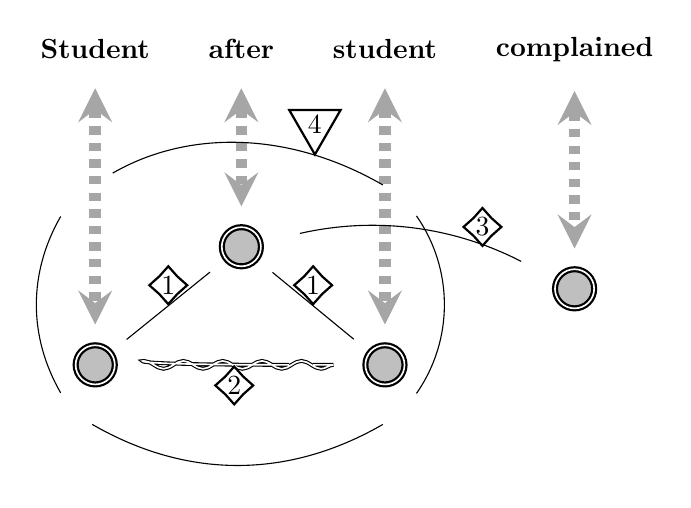
\begin{tikzpicture}

%\tikzset{snake it/.style={decorate, decoration=snake, segment length=5mm, amplitude=15mm}}

%\draw

%\node [s1] at (0,0) {Student};

\node (s1) at (1,1) {\textbf{Student}};
\node (after) [right=5mm of s1] {\textbf{after}};
\node (s2) [right=5mm of after] {\textbf{student}};
\node (complained) [right=5mm of s2] {\textbf{complained}};

\node (s1Rep) [double,draw=black,shape=circle,thick,fill=gray!50,inner sep=.5em,below=3.5cm of s1] {};
\node (afterRep) [double,draw=black,shape=circle,thick,fill=gray!50,inner sep=.5em,below=2cm of after] {};
\node (s2Rep) [double,draw=black,shape=circle,thick,fill=gray!50,inner sep=.5em,below=3.5cm of s2] {};
\node (complainedRep) [double,draw=black,shape=circle,thick,fill=gray!50,inner sep=.5em,below=2.5cm of complained] {};

\draw [ |-,-|, <->, line width = .8mm, draw=gray!70, 
 dashed, double equal sign distance, >= stealth, shorten <= .25cm, shorten >= .25cm ]
 (s1) to (s1Rep);

\draw [ |-,-|, <->, line width = .8mm, draw=gray!70, 
 dashed, double equal sign distance, >= stealth, shorten <= .25cm, shorten >= .25cm ]
(after) to (afterRep);
 
\draw [ |-,-|, <->, line width = .8mm, draw=gray!70,  
 dashed, double equal sign distance, >= stealth, shorten <= .25cm, shorten >= .25cm ]
(s2) to (s2Rep);

\draw [ |-,-|, <->, line width = .8mm, draw=gray!70, 
 dashed, double equal sign distance, >= stealth, shorten <= .25cm, shorten >= .25cm ]
(complained) to (complainedRep);
 
\draw [shorten <= .25cm, shorten >= .25cm ] 
(afterRep) to node [draw=black,shape = star,star points=4,thick,inner sep = 0mm, above] {1} (s1Rep);

\draw [shorten <= .25cm, shorten >= .25cm ] 
(afterRep) to node [draw=black,shape = star,star points=4,thick,inner sep = 0mm,above] {1} (s2Rep);

\node (s1E) [left=-2mm of s1Rep.east]{};
\node (s2E) [left=1mm of s2Rep.west]{};

\draw [shorten <= 2cm, shorten >= .3cm, double, % bend left = 5, 
decorate, decoration={snake, segment length=5mm, amplitude=.5mm}] %, amplitude=15mm]  
(s1E) to node [draw=black,shape = star,star points=4,thick,inner sep = 0mm, below] {2} (s2E);

\draw [shorten <= .5cm, shorten >= .5cm ] 
(afterRep) edge [bend left=20,looseness=1] node [draw=black,shape = star,star points=4,thick,inner sep = 0mm, 
 above, near end ] {3} (complainedRep);

\node (frameTopLeft) [below left = 1.5cm and -.65 cm of s1] {};
\node (frameBottomLeft) [below = 2.5cm of frameTopLeft] {};
\node (frameBottomRight) [right = 3.95cm of frameBottomLeft] {};
\node (frameTopRight) [above = 2.5cm of frameBottomRight] {};

\draw [shorten <= 0.15cm, shorten >= 0.15cm ] 
(frameTopLeft) edge [bend right=30,looseness=1] (frameBottomLeft);

\draw [shorten <= 0.15cm, shorten >= 0.15cm ] 
(frameBottomLeft) edge [bend right=30,looseness=1] (frameBottomRight);

\draw [shorten <= 0.15cm, shorten >= 0.15cm ] 
(frameBottomRight) edge [bend right=35,looseness=1] (frameTopRight);

\draw [shorten <= 0.15cm, shorten >= 0.45cm ] 
(frameTopRight) edge [bend right=30,looseness=1]
node [draw=black,shape = regular polygon,regular polygon sides=3,thick,inner sep = .2mm, 
above, near start, shape border rotate = 180] {4} (frameTopLeft);

%node [draw=black,shape = star,star points=4,thick,inner sep = 0mm, above, 
%bend left=100,looseness=3] {3}

%;


\end{tikzpicture}
\end{minipage}

\hspace{0.1\textwidth}
\begin{minipage}{0.8\textwidth}
			\renewcommand{\labelitemi}{$\blacklozenge$}
	
\begin{itemize}\setlength\itemsep{-.3em}
\item 1 \hspace{12pt}  Head/dependent relation
\item 2 \hspace{12pt}  Argument repetition ({}\BlankAfterBlank{} idiom)
\item 3 \hspace{12pt}  Propositional completion ({}\VisNtoS{})	
			\renewcommand{\labelitemi}{$\blacktriangledown$}
\item 4 \hspace{12pt}  Phrase (modeled as applicative structure), typed as {}\NPl{} 
\end{itemize}
\end{minipage}
\end{figure}   
As this shows, the \q{Student after Student} idiom can be notated as, say, 
\AfterNSingAndNSingToNPl{} (using \NSing{} and \NPl{} to mean singular 
and count-plural nouns, respectively), but with the special case that the \q{argument} to 
\i{after} is repeated in both positions, suggesting an unusual degree of repetition, 
something frustratingly recurrent: \i{He went on and on}; \i{Car after car passed 
us by}; \i{Time after time I got turned down}.
Although I have no problem
treating these constructions as idiomatic plurals, I also contend (on the 
premise of phrase-overlap) that the dependent constituents in the \BlankAfterBlank{} 
construction can be hooked to other phrases as well (which is why 
\q{and [their/his/her] parents} can also be singular, in this case).  I dwell on 
this example because it shows how type/functional accounts of phrase structure 
can be useful even if we treat phrases more as frames which overlay linguistic 
structure, not as rigid compositional isolates.  Each \q{students} variation uses 
morphology to nudge cognitive attention in one direction or another, toward events or the 
degree to which events are representative of some global property (here of 
a student body), or both.  The \NSingToNPl{} transformation is not \i{the} 
morphosyntactic meaning, but instead the skeleton on which the full meaning 
(via cognitive schema) is designed, its hints solicited.
}
\p{If this analysis has merit, it suggests that a \CAG{} 
approach to phrases like \i{many students} or \i{student after student} 
(singular-to-plural or plural-to-plural mappings) should be understood not just 
as functions among Part of Speech (\POS{}) types but as adding cognitive shading, foregrounding 
or backgrounding cognitive elements like events or typicality in some context.  
In other words, \i{many students} is type-theoretically \NtoN{} or \NpltoNpl{}; 
but, in more detail, it adds a kind of cognitive rider attached to the mapping which focuses 
cognition in the subsequent discourse onto events (their recurrence and temporal distribution); 
similarly \q{student after student} has a \q{rider} suggesting more of a temporal 
unfolding.  The second form implies not only that many students complained, but that 
the events of these complainings were spread out over some stretch of time.  
Each such functional application (mappings between \POS{} understood as linguistic types) 
produces not only a resulting \POS{} \q{type}, but also a reconfiguration of cognitive 
attitudes toward the relevant situation and context.  
Language users have many ways to craft a sentence with similar meanings, and arguably one 
task for linguistic analysis is to model the space of choices which are available in a 
given situation and represent what specific ideas and effects are invoked by one 
choice over others.  It would be an argument in favor of Dependency Grammar if 
Dependency-oriented representational models, like Link Grammar, prove to be 
especially adept in this modeling.  
}
\p{In this analysis, I am already switching to functional and type notions that will be 
discussed in greater detail below; my current emphasis is on link grammar as a syntactic 
conception, although I have also tried to argue that separating syntax from semantics 
can be at most provisional.  Inter-word \q{link pairs} are vehicles for expressing 
syntactic rules (like singular/plural agreement) but are also a ground level for 
semantic analysis, since we can explain how semantic nuances are carried, in 
specific sentences, by the actual link-pairs in evidence (violations to 
agreement norms, for example).  These semantic nuances in turn can be given 
cognitive interpretations, revealing the syntax-semantics-cognition pattern
which I am sketching here through specific perspectives like Link Grammar and 
Type Theory.  Returning to the initial grammatic stage of analysis, however, 
my tactics for contrasting overall Dependency and Phrase-Structure paradigms 
rest on an implicit picture of how theories should be evaluated.  
While such a picture is probably fairly consistent across perspectives, it is still worth 
making a little more explicit.  
}
\subsection{Explanation and Formality}
\p{Both Dependency and Phrase Structure grammars 
presuppose that the fundamental exposition and achievement of their theory involves 
formal transformation of linguistic givens, resulting in a more complex data structure 
which, to the extent that the theory is correct and useful, models something 
of the inner structure of language (\i{qua} abstract formal system and/or cognitive phenomenon).  
The \q{data structure} might be a phrase-structure \q{tree} or a graph-like dependency 
\q{linkage}, but while these representations have different form they share certain 
criteria: they are formally describable systems which allow some structures but reject others; 
they are rigorous enough to be given a mathematical (e.g., algebraic) definition; 
and they can be expressed in computer code which builds these structures out of 
Natural Language artifacts, can verify that an instance of the relevant data structures 
satisfies the system rules, and can execute operations which modify the structures.  
The phrase trees or word-link graphs are \q{formal substrata} which encapsulate Natural Language 
patterns but also are rigidly mathematical and computational.  How thoroughly these substrata 
capture linguistic meaning, is therefore directly relevant to questions of whether and 
in what degree natural language itself, as social and cognitive, is also formal and computational.
}
\p{Translating NL content into (say) a linked-grammar graph does not make software capable 
of \q{understanding} language.  If Dependency Grammar is a reasonable foundation 
for linguistics in general, then properly parsing sentences into their 
auxiliary graphs is, at most, a step in the direction toward \q{understanding}.  
Even this may beg the question of what constitutes a \q{correct} parse: when writing 
real-world code, language engineers appear to rely principally on their own intuitions, based 
on their familiarity with the underlying theory, the idea they have of what a 
\i{correct} \q{re-presentation} looks like (for link grammar, of the correct collection of 
link types between the various words).  They then add code to ensure that this representation 
is indeed identified by the software in specific examples, and try to do so in such a way 
as to generalize to other examples.  This methodology can be gleaned from observing internet chat 
sites and other informal research venues; one can witness developers painstakingly constructing 
systems which \q{work right} in the sense of producing the interpretation for each sentence 
which corresponds with what the human linguists perceive, even for sentences which the 
software has never encountered before.  The code is considered reliable the more that 
new sentences are \q{correctly} parsed.  Again, \q{correctly} here means, conformant to 
linguists' own interpretations; insofar as these are subjective, such conformance is not 
conclusive evidence that the transformational algorithms are \q{correct}.   
}
\p{In order to assess linguistic \q{competence} (or whatever computational ability may simulate it), 
it is needed to check specific \q{behavior} and compare it to some expectation.  The gold standard 
for linguistic behavior is just participating in a linguistic community, judged by the community 
at large as fully competent and included.  Unfortunately, however \mdash{} at least for those who 
want to profit from Artificial Intelligence \mdash{} achieving true \q{language-like behavior} may be 
impossible.  Scholarship therefore has to turn toward more limited notions of 
competence, such as representational transformation of sentences \mdash{} but since 
each theory has its own picture of what sentences should be transformed \i{into}, 
the justification of competence measures can be circular.  It is the theory which 
dictates how the software should act, and the software is deemed \q{intelligent} if it 
acts accordingly.  We can be skeptical of such non-theory-neutral conceptions of 
\q{intelligence}.  Nonetheless it does count 
in theories' favor if they both propose accounts of language structure which 
are independently defensible and also can produce computing systems that 
reliably and without external direction map language onto those structures.  
Language-like behavior then involves producing a transformed representation of 
language embodying a particular theoretical conception of 
linguistic \q{deep structure}.
}
\p{It would serve Computational-Linguistic theories still further to create systems 
that demonstrate behavior which is \q{language-like} on terms less wedded to their 
own hypotheses.  More satisfying definitions of linguistic behavior would involve intuitions 
of language users in general, not just language experts.  For example, document classifiers 
\mdash{} which typically use statistical analysis to predict which topic will be deemed most 
relevant for documents like news stories and technical articles \mdash{} again illustate a kind 
of transformational representation, converting Natural Language to a formal data structure 
(in this case a relatively simple one, naming one or multiple topics from a predefined list).  
In this case however a broad user public can provide feedback on how well the system performs.  
For another example, artificial translators map language onto formal structures but then 
attempt an opposite map, translating the formalized representation into natural-seeming 
expressions in a different language.  This case is different in that formal representation is 
an intermediary rather than end point of the transformation, but like document classifiers it 
is a kind of behavior whose effectiveness can be judged by a large community of speakers.  
People who interact with text \q{chat} bots, or talking robots, and feel that the experience 
is similar to talking with another person, are also providing evidence of more complete and 
larger-scale language-like behavior.  Again, though, it is not now and may never be possible 
to engineer intelligent behavior to this level of perfection.  Existing language \AI{} platforms 
are flawed but useful, which suggests both that formal re-presentation is an important 
step toward language understanding but also that attempts to use these formalisms as a springboard 
to more holistic behavior \mdash{} like automated translation, but also extracting practical 
information, or gleaning emotion and sentiment \mdash{} are missing something essential.  
Doing useful things with or gleaning useful insight from the re-presentational target structures 
appears to be a separate problem from that of generating them \mdash{} which calls into question the 
degree to which the target structures sufficiently encapsulate linguistic meaning, 
even if they reveal structures which are essential to linguistic meaning.  
}
\p{This does not have to mean that Natural Language Processing is basically impossible, only 
that more modest criteria of \q{correct} \NLP{} systems need to be adopted.  This is complicated 
by the fact that artifical language behavior can be flawed but meaningful: \q{Urine shift one 
step forward} is an awkward English sentence but its meaning seems clear enough 
(this real example comes from a shopping center in New York's Flushing, Queens Chinatown).
We have an intuition that some expressions are \q{incorrect} but not so completely 
off-base that they fail to signify anything at all \mdash{} but in this case we need 
criteria for how a linguistic performance can be both incorrect \i{and} nonetheless coherent.
}
\p{These issues influence any theory which approaches linguistic competence from the 
viewpoint of formal re-presentations, and therefore effectively all branches of 
Computational Linguistics.  The reigning assumption appears to be that transformational 
representation which converts language to theory-regulated data structures, for which 
in many cases the transformation achieved by mechanical algorithms matches that 
intuited as most accurate by human experts, serves as \i{prima facie} evidence of 
something like computationally-engineered  \q{intelligent (language) behavior}.  
This leaves room for language-like behavior to productively replicate dimensions 
of language understanding while also being very incomplete: language-like relative 
to experts' opinions on deep linguistic structure, not real-world communication.  
Structures like link grammar graphs can be essential formal substrata that linguistic expression 
relies on to achieve communication, without being the sole medium of this expression.
}
\p{My arguments so far have used Link Grammar as a representative example 
of \q{transformational representation} where a computational system 
can be judged to reveal some level of language competence, some 
kind of \q{language like behavior}, insofar as it translates natural 
language expressions to data structures conformant to Dependency 
Grammar (and particularly Link Grammar) theory.  
As I also just argued, performance \visavis{} structural transformation 
may be only tangential to human language, so whatever theory is 
built up needs a separate, more philosophical or metatheoretical analysis 
to consider how the theory is purported to engage with its phenomena.  
But I now take this as a starting point for pivoting the discussion from
grammar to semantics; and will defer until after that speculating 
on philosophical implications of the theory thus extended.
}

\section{Link Grammar and Type Theoretic Semantics}
\p{From one perspective, grammar is just a 
most top-level semantics, the primordial Ontological division of language into designations of 
things or substances (nouns), events or processes (verbs), qualities and attributes (adjectives), 
and so forth.  Further distinctions like count, mass, and plural nouns add 
semantic precision but arguably remain in the orbit of grammar (singular/plural 
agreement rules, for example); the question is whether semantic detail gets 
increasingly fine-grained and somewhere therein lies a \q{boundary} between syntax and 
semantics.  The mass/count distinction is perhaps a topic in grammar more so than 
semantics, because its primary manifestation in language is via agreement 
(\i{some} wine in a glass; \i{a} wine that won a prize; \i{many} wines 
from Bordeaux).  But are the distinctions between natural and constructed objects, 
or animate and inanimate kinds, or social institutions and natural 
systems, matters more of grammar or of lexicon?  Certainly they engender 
agreements and propriety which appear similar to 
grammatic rules.  \q{The tree wants to run away from the dog} sounds wrong \mdash{} because 
the verb \q{want}, suggestive of propositional attitudes, seems incompatible with 
the nonsentient \q{tree}.  Structurally, the problem with this sentence seems analogous 
to the flawed \q{The trees wants to run away}: the latter has incorrect singular/plural linkage, 
the former has incorrect sentient/nonsentient linkage, so to speak.  But does this 
structural resemblance imply that singular/plural is as much part of semantics as grammar, or 
sentient/nonsentient as much part of grammar as semantics?  It is true that there are no 
morphological markers for \q{sentience} or its absence, at least in English \mdash{} except 
perhaps for \q{it} vs. \q{him/her} \mdash{} but is this an accident of English or revealing 
something deeper?
}
\p{To explore these questions it is first necessary to consider how a grammar theory can be 
extended to and/or connected with a formal or, to some measure, informal semantics.  
Here I will present one approach to make this extension \visavis{} Link Grammar.
}
\p{Insofar as grammatic categories do provide a very basic \q{Ontological} viewpoint, 
it is reasonable to build semantic formalization on top of grammar theories.  
Link Grammar, for example, explicitly derives \q{link types} \mdash{} species of word-to-word 
relations \mdash{} by appeal to \q{Categorial} grammars which define parts of 
speech in terms of their manner of composition with other, more \q{fundamental} parts 
of speech \cite{Kiselyov}, \cite{Rossi}, \cite{MartinPollard}.  The most primordial 
grammatic categories are generally seen to be nouns and 
\q{propositions} (self-contained sentences or sentence-parts which assert individual states of 
affairs), and categories like verbs and adjectives are derived on their basis.  For example, a 
verb \q{combines} with a noun to produce a proposition.  \i{Students} is an abstract 
concept; \q{Students complained}, tieing the noun to a verb, tethers the concept to an 
assertorial flesh, yielding something that expresses a belief or observation.  
Meanwhile, Categorial Grammar models not only the semantic transition from abstract to concrete, but 
surface-level composition: in English and other \SVO{} language for example the verb should 
immediately follow the noun; in German and all \SVO{} languages the verb tends the come 
last in a sentence, and can be well apart from its subject.  The semantic pattern in the 
link is how the verb/noun pair yields a new semantic category (propositional) whereas the 
grammatic component lies in how the link is established relative to other words 
(to the left and not the right, for example, and whether or not the words are adjacent).  
}
\p{Assuming that surface-level details can be treated as grammar rules and abstracted from 
the semantics, we can set aside Categorial Grammar notions like connecting 
\q{left} vs. \q{right} or \q{adjacent} (near) vs. \q{nonadjacent} (far).  
With this abstracting, Categorial Grammar becomes similar 
to a Type-Theoretic Semantics which recognizes, in Natural Language, operational 
patterns that are formally studied in mathematics and computer science
\cite{ZhaohuiLuo}, \cite{MaillardClarkGrefenstette}, 
\cite{ZhaohuiLuo}, \cite{Pollard}, \cite{MeryMootRetore}.
A verb, for example, 
\i{transforms} a noun into a sentence or proposition (at least an intransitive verb; 
other kinds of verbs may require two, or even three nouns).  In some schematic sense a 
verb is analogous to a mathematical \q{function}, which \q{takes} one or more nouns 
and \q{yields} propositions, much like the \q{square} function takes a real number and 
yields a non-negative real number.  To make this analogy useful, however, 
it is necessary to clarify how \q{types} in a mathematical or computational 
context may serve as appropriate metaphors for syntactic and/or semantic groupings in language.
}
\subsection{Types, Sets, and Concepts}
\p{Most Computer Science rests on types rather than (for example) sets, 
because abstract reasoning about data types 
requires some abstraction from practical limitations about how particular values may be 
digitally encoded.  
Types can be defined as sets of both values and 
\q{expectations} \cite{MathieuBouchard} (meaning assumptions which may be made about 
all values covered by the type); alternatively, we can (perhaps better) consider types as 
\i{spaces} of values.  Types' extensions have internal structure; there 
can be \q{null} or \q{invalid} values, default-constructed values, and 
so forth, which are \q{regions} of type-space and can 
be the basis of topological or Category-Theoretic rather than 
set-based analyses of type-extension.  Also, expectations intrinsically include 
functions which may be \q{called on} types.  There is definitional interdependence 
between types and functions: a function is defined in terms of the types it accepts as parameters and 
returns \mdash{} rather than its entire set of possible inputs and outputs, which can 
vary across computing environments.  These are some reasons why in theoretical 
Computer Science types are not \q{reduced} to underlying sets; instead, extensions 
are sometimes complex spaces that model states of, or internal organization of comparisons 
among, type instances.
}
\p{An obvious paradigm is organizing type-extensions around prototype/borderline
cases \mdash{} there are instances which are clear examples of types and
ones whose classification is dubious.  I will 
briefly argue later, however, that common resemblance is not always a good marker
for types being well-conceived \mdash{} many useful concepts are common
precisely because they cover many cases, which makes defining
\q{prototypes} or \q{common properties} misleading; this reasoning
arguably carries over to types as well.  Also, sometimes the clearest
\q{representative} example of a type or concept is actually not a
\i{typical} example: a sample latter or model home is actually not (in
many cases) a real letter or home.  So resemblance-to-prototype is at
best one kind of \q{inner organization} of concepts' and types' spaces
of extension.  Computer Science develops other 
pictures of types' \q{state space}, reflecting the trajectory of symbols 
or channels which hold type instances, which at different moments in time 
become initialized \mdash{} acquiring a value obtained from a \i{constructor} 
function (one \q{type space region} is then demarcated by which values 
can be direct results of constructors) \mdash{} then possibly subject to change in the value they hold, and finally 
(often) transitioning to a state where the held value is no longer \q{valid}.\footnote{Managing the \q{lifetime} of values from many types, especially \q{pointer} types 
(that hold a numeric value representing the current memory address of some other value),
has been a notorious source of programming errors, especially in older computer 
languages.  Of late, also, data types often need to be designed to minimize the 
risk of data corruption, theft, and malicious code.  For these reasons, 
Cybersecurity takes particularly interest in studying types' extensions and transitions 
between different values (morphisms within a type space) to formally describe 
states or state-transitions which are security vulnerable.
}  Type \i{spaces} have potentially complex patterns of regions and equivalence classes of 
inter-value mappings (in the sense of behavioral equivalence relative to 
code analysis, testing, or security) 
\mdash{} the \i{conceptual} properties of types are expressed in the 
\i{internal structuration} of their associated state-space.  Putting this in mathematical 
language, an in-depth treatment of types cannot work \q{in the Category} of 
sets, even for basic type-extension, but rather (for instance) the 
Category of Topological Spaces.
}
\p{Moreover, expectations in a particular case 
may be more precise than what is implied by the type itself \mdash{} it is erroneous 
to assume that a proper type system will allow a correct \q{set of values} to 
be stipulated for each point in a computation (the kind of contract enforced via 
by documentation and unit testing).  So state-space in a given context may include many
\q{unreasonable} values, implying that within the overall space there is a \q{reasonable}
subspace, except that this subspace may not be crisply defined.  
A value representing someone's age may be assigned 
a type for which a legal value is, say, 1000 years, which is obviously unreasonable 
\mdash{} the conceptual role served by the \i{particular} use of a type in some context can 
be distinct from the entire space of values exhibited by the type.  It is possible to 
construct types which are narrowed down to more precise ranges, but in many cases this is 
unnecessary or poorly motivated: while 1000 years is clearly too large for an age, 
it would be arbitrary to specify a \q{maximum allowed} age (recall that assuming a 
\q{maximum allowed} year of 1999 \mdash{} so that the year in decimal only required two digits 
\mdash{} led to costly reprogramming of archaic legacy code during \YtwoK{}).  
In this kind of situation programmers 
usually assign types based on properties of binary representation \mdash{} what number of 
binary digits is optimal for memory and/or speed, even if this allows \q{absurd} values 
like 1000 years old.  Run-time checks, rather than type restrictions, may be used to 
flag nonsensical data and prevent data corruption.  In these scenarios, types represent a 
compromise between \i{concepts}, which can be fuzzy and open-ended, and 
\i{sets}, which conceptually are nothing more than the totality of their extension.\footnote{Nevertheless, there is interesting (and potentially practically useful) research in 
how formal type-constructions model conceptual organization: for example, 
\Gardenfors{} Conceptual Space Theory has seen formal implementations 
\cite{RaubalAdams}, and it is very interesting to juztapose 
scientific and mathematical treatments of Conceptual Spaces (as in \cite{Strle} or 
\cite{Zenker}) with mathematical (e.g., topological) thoeries of 
data types \cite{Escardo}, \cite{StellConvexivity}.
}
}
\p{Sets, concepts, and types represent three different primordial thought-vehicles for 
grounding notions of logic and meaning.  To organize systems around \i{sets} is 
to forefront notions of inclusion, exclusion, extension, and intersection, 
which are also formally essential to mathematical logic and undergird the 
classical interdependence of sets, logic, and mathematics.\footnote{Recent work in mathematics, however (partly 
under the influence of computational proof engines and foundations research 
like Homotopy Type Theory) shows that type and/or Category theory 
may replace sets as a groundlevel for logico-mathematical reasoning (if 
not notation) in the future \cite{HOTT} (It is worth pointing out that 
despite their similar ordinary meanings, mathematically \i{type} is much different 
from \i{Category} even though these respective theories can be usefully integrated).
}
To organize systems around \i{concepts} is to forefront practical engagement 
and how we mold conceptual profiles, as collections of ideas and pragmas, 
to empirical situations.  To organize systems around \i{types} is to forefront 
\q{functions} or transformations which operate on typed values, the interrelationships 
between different types (like subtypes and inclusion \mdash{} a type can itself 
encompass multiple values of other types), and the conceptual abstraction 
of types themselves from the actual sets of values they may exhibit 
in different environments.  Sets and types are 
formal, abstract phenomena; whereas concepts are characterized by 
gradations of applicability, and play flexible roles in thought and language.  
The cognitive role of concepts can be discussed with some rigor, but there is a 
complex interplay of cognitive schema and practical engagements which 
would have to be meticulously sketched in many real-world scenarios, if 
our goal were to translate conceptual reasoning to formal structures 
on a case-by-case basis.  We can, however, consider in general 
terms how type-theoretic semantics can capture conceptual structures 
as part of the overall transitioning of thoughts to langauge.
}
\p{A concept does not merely package up a definition, like \q{restaurant} as 
\q{a place to order food}; instead concepts link up with other concepts 
as tools for describing and participating in situations.  Concepts are 
associated with \q{scripts} of discourse and action, and find their 
range of application through a variegated pragmatic scope.  
We should be careful not to overlook these pragmatics, and 
assume that conceptual structures can be simplistically 
translated to formal models.  
Cognitive Linguistics critiques 
Set-Theoretic or Modal Logic reductionism (where a concept is just a set 
of instances, or an extension across different possible worlds) \mdash{} George Lakoff and Mark Johnson, 
prominently, argue for concepts' organization around 
prototypes (\cite[p. 18]{LakoffJohnson}; \cite[p. 171, or p. \textit{xi}]{Johnson}) 
and embodied/enactive patterns of interaction (\cite[p. 90]{LakoffJohnson}; 
\cite[p. 208]{Johnson}).  
Types, by contrast, at least in linguistic applications of type theory, are abstractions 
defined in large part by quasi-functional notions of phrase struture.  
Nevertheless, the \i{patterns} of how types may inter-relate 
(mass-noun or count-noun, sentient or non-sentient, and so forth) 
provide an infrastructure for conceptual understandings to be 
encoded in language \mdash{} specifically, to be signaled by which typed 
articulations conversants choose to use.  A concept like 
\i{restaurant} enters language with a collection of understood 
qualities (social phenomena, with some notion of spatial location and 
being a \q{place}, etc.) that in turn can be marshaled by sets of 
allowed or disallowed phrasal combinations, whose parameters 
can be given type-like descriptions.  Types, in this sense, 
are not direct expressions of concepts but vehicles for 
introducing concepts into language.
}
\p{Concepts (and types also) are not cognitively the same as their 
extension \mdash{} the concept \i{restaurant}, I believe, is distinct from  
concepts like \i{all restaurants} or \i{the set of all restaurants}.
This is for several reasons.  First, Concepts can be pairwise different 
not only through their instances, but because they highlight different 
sets of attributes or indicators.  The concepts \q{American President} and \q{Commander in Chief} 
refer to the same person, but the latter foregrounds a military role.  
Formal Concept Analysis considers \i{extensions} and \q{properties} 
\mdash{} suggestive indicators that inhere in each 
instance \mdash{} as jointly (and co-dependently) determinate: concepts 
are formally a synthesis of instance-sets and property-sets \cite{YiyuYao}, 
\cite{Belohlavek}, \cite{Wille}.  Second, 
in language, clear evidence for the contrast between \i{intension} and 
\i{extension} comes from phrase structure: certain constructions specifically 
refer to concept-extension, triggering a mental shift from thinking of the 
concept as a schema or prototype to thinking of its extension (maybe in some context).  
Compare these sentences: 
\sentenceexamples{\sentenceexample{Tigers in that park are threatened by poachers.}
\sentenceexample{Young tigers are threatened by poachers.}
}
Both sentences focus a conceptual lens in greater detail than \i{tiger} in general, but 
the second does so more intensionally, by adding an extra indicative criterion; while 
the former does so extensionally, using a phrase-structure designed to operate on 
and narrow our mental construal of \q{the set of all tigers}, in the sense of 
\i{existing} tigers, their physical place and habitat, as opposed to 
the \q{abstract} (or \q{universal}) type.  So there is a familiar semantic 
pattern which mentally transitions from a lexical type to its extension and 
then extension-narrowing \mdash{} an interpretation that, if accepted, clearly 
shows a different mental role for concepts of concepts' \i{extension} than the 
concepts themselves.
}
\p{There is a type-theoretic correspondence between intension and 
extension \mdash{} for a type \Tnoindex{} there is a corresponding \q{higher-order} type 
of \i{sets} whose members are \Tnoindex{}.\footnote{Related constructions are the type of \i{ordered sequences} of \Tnoindex{}; 
unordered collections of \Tnoindex{} allowing repetition; and stacks, queus, and 
deques (double-ended queues) as \Tnoindex{}-lists that can grow or shrink 
at their beginning and/or end.
}  If we take this (higher-order) 
type gloss seriously, the extension of a concept is not its \i{meaning}, but a  
different, albeit interrelated concept.  Extension is not definition.  
\q{Tiger} does not mean \i{all tigers} (or \i{all possible tigers}) \mdash{} though arguably 
there are concepts \i{all tigers} and \i{all restaurants} (etc.) along with the concepts 
\i{tiger} and \i{restaurant}.  Concepts, in short, do not mentally signify sets, or 
extensions, or sets-of-shared-properties.  Concepts, rather, are cognitive/dialogic tools.  
Each concept-choice, as presentation device, 
invites its own follow-up.  \i{Restaurant} or \i{house} have meaning not via  
idealized mental pictures, or proto-schema, but via kinds of things 
we do (eat, live), of conversations we have, of qualities we deem relevant.  Concepts do not 
have to paint a complete picture, because we use them as part of ongoing situations 
\mdash{} in language, ongoing conversations.  Narrow concepts \mdash{} which may best exemplify 
\q{logical} models of concepts as resemblance-spaces or as rigid designators to 
natural kinds \mdash{} have, in practice, fewer use-cases \i{because} there 
are fewer chances for elaboration.  Very broad concepts, on the other hand, can have, 
in context, too \i{little} built-in \i{a priori} detail.  
(We say \q{restaurant} more often than \i{eatery}, and 
more often than \i{diner}, \i{steakhouse}, or \i{taqueria}).  Concepts dynamically play 
against each other, making \q{spaces} where different niches of meaning, including 
levels of precision, converge as site for one or another.  Speakers need freedom to choose 
finer or coarser grain, so concepts are profligate, but the most oft-used trend toward middle 
ground, neither too narrow nor too broad.  \i{Restaurant} or \i{house} are useful because they are noncommittal, inviting more detail.  
These dynamics govern the flow of inter-concept relations (disjointness, subtypes, partonymy, etc.). 
}
\p{Concepts are not rigid formulae (like instance-sets or even attributes fixing when 
they apply); they are mental gadgets to initiate and 
guide dialog.  Importantly, this 
contradicts the idea that concepts are unified around instances' similarity (to each other or 
to some hypothetical prototype): concepts have avenues for contrasting 
different examples, invoking a \q{script} for further elaboration, or for building temporary filters 
(\q{Let's find a restaurant that's family-friendly}; allowing such one-off narrowing is a feature 
of the concept's flexibility).
No less important, than acknowledged similarities across all instances, are well-rehearsed ways 
\visavis{} each concept to narrow scope by marshaling lines of \i{contrast}, of \i{dissimilarity}.  
A \i{house} is obviously different from a \i{skyscraper} 
or a \i{tent}, and better resembles other houses; but there are also more nontrivial \i{comparisons} 
between houses, than between a house and a skyscraper 
or a tent.  Concepts are not only spaces of similarity, but of \i{meaningful kinds of differences}.
}
\p{To this account of conceptual spaces we can add the conceptual matrix spanned by 
various (maybe overlapping) word-senses: to \i{fly}, for example, names 
not a single concept, but a family of concepts all related to airborn 
travel.  Variations highlight different features: the path of flight (\i{fly to Korea}, \i{fly over the mountain}); 
the means (\i{fly Korean air}, \i{that model flew during World War II}); 
the cause (\i{sent flying (by an explosion)}, \i{the bird flew away (after a loud noise)}, 
\i{leaves flying in the wind}).  Words allow different use-contexts 
to the degree that their various \i{senses} offer an inventory of aspects for 
highlighting by \i{morphosyntactic} convention.  Someone who says \i{I hate to fly} is not 
heard to dislike hand-gliding or jumping off mountains.\footnote{People, unlike birds, do not fly \mdash{} so the verb, used intransitively 
(not flying \i{to} somewhere in particular or \i{in} something in particular), 
is understood to refer less to the physical motion and more to the socially 
sanctioned phenomenon of buying a seat on a scheduled flight on an airplane. The construction 
highlights the procedural and commercial dimension, not the physical mechanism and 
spatial path.  But it does so \i{because} we know human flight is 
unnatural: we can poetically describe how the sky is filled with flying leaves or birds, 
but not \q{flying people}, even if we are nearby an airport.  
Were \q{flying people} used jokingly, it would be in bad taste, like
\q{cat all over all over the driveway} from Pinker 
\cite{Pinker} on page 119 and Langacker's \q{Nouns and Verbs} \cite{Langacker87} on page 67.
}  Accordant variations 
of cognitive construal (attending more to mode of action, or path, or motives, etc.), 
which are elsewhere signaled by grammatic choices, are also spanned by a conceptual 
space innate to a given word: senses are finer-grained meanings availing themselves to one construal or another.    
}
\p{So situational construals can be signaled by word- and/or 
syntactic form choice (locative, benefactive, direct and indirect 
object constructions, and so forth).  Whereas conceptual organization 
often functions by establishing classifications, and/or invoking 
\q{scripts} of dialogic elaboration, cognitive structure tends to apply more 
to our attention focusing on particular objects, sets of objects, events, or 
aspects of events or situations.  \i{Conceptual} is more abstract and belief-oriented; 
\i{Cognitive} is more concrete and phenomenological.  Concepts organize our 
\q{background knowledge} \cite{SmithMcIntyre}; cognitions allow it to be latent 
against the disclosures of material consciousness 
\cite{DavidWoodruffSmith}, \cite{DavidWoodruffSmithChapter}, 
\cite{JordanZlatev}, \cite{SeanDorranceKelley}. 
So the contrast between singular, mass-multiples, and count-multiples, 
among nouns, depends on cognitive 
construal of the behavior of the referent in question (if singular, its 
propensity to act or be conceived as an integral whole; if multiple, its 
disposition to either be divisible into discrete units, or not).  
Or, events can be construed in terms of their causes 
(their conditions at the outset), or their goals (their conditions at 
the conclusion), or their means (their conditions in the interim).  
Compare \i{attaching} something to a wall (means-focused) to 
\i{hanging} something on a wall (ends-focused); \i{baking} a cake 
(cause-focus: putting a cake in the oven with deliberate intent to cook it) 
to \i{burning} a cake (accidentally overcooking it).\footnote{We can express 
an intent to bake someone a cake, but not (well, maybe comedically) to 
\i{burn} someone a cake (\q{burn}, at least in this context, implies 
something not intended); however, we \i{can} say 
\q{I burnt your cake}, while it is a little jarring to say 
\q{I baked your cake} \mdash{} the possessive implies that some 
specific cake is being talked about, and there is less apparent reason 
to focus on one particular stage of its preparation (the baking) once 
it is done.  I \i{will} bake a cake, in the future, uses 
\q{bake} to mean also other steps in preparation (like \q{make}), while, 
in the present, \q{the cake \i{is} baking} emphasizes more its 
actual time in the oven.  I \i{baked your cake} seems to focus 
(rather unexpectedly) on this specific stage even after it is completed, 
whereas \i{I baked you a cake}, which is worded as if the recipient 
did not know about the cake ahead of time, apparently uses \q{bake} in 
the broader sense of \q{made}, not just \q{cooked in an oven}.  
Words' senses mutate in relation to the kinds of situations where they are used 
\mdash{} why else would \i{bake} mean \q{make}/\q{prepare} in the past or future tense but 
\q{cook}/\q{heat} in the present?  
}
These variations are not random assortments of polysemous words' senses: 
they are, instead, rather predictably distributed according 
to speakers' context-specific knowledge and motives.  
}
\p{I claim therefore that \i{concepts} enter language complexly, influenced by 
conceptual \i{spaces} and multi-dimensional semantic and syntactic selection-spaces.  
Concepts are not simplistically \q{encoded} by types, as if for 
each concept there is a linguistic or lexical type that just 
disquotationally references it \mdash{} that the type \q{tiger} means the concept 
\i{tiger} (\q{type} in the sense that type-theoretic semantics would model lexical 
data according to type-theoretic rules, such as \i{tiger} as subtype of \i{animal} or 
\i{living thing}).  
Cognitive schema, at least in the terms I just laid out, select particularly 
important gestalt principles (force dynamics, spatial frames, action-intention) 
and isolate these from a conceptual matrix.  On this basis, we can argue that 
these schema form a precondition for concept-to-type association; or, 
in the opposite logical direction, that language users' choices to employ 
particular type articulations follow forth from their prelinguistic 
cognizing of practical scenarios as this emerges out of collections 
of concepts used to form a basic understanding of and self-positioning within them.
}
\p{In this sense I called types \q{vehicles} for concepts: not that types \i{denote} 
concepts but that they (metaphorically) \q{carry} concepts into language, as a bus 
carries people into a city.  \q{Carrying} is enabled by types' semi-formal rule-bound 
interactions with other types, which are positioned to capture concepts' variations and 
relations with other concepts.  
To express a noun in the benefactive case, for example, which can be seen as attributing to 
it a linguistic type consistent with being the target of a benefactive, 
is to capture the concept in a type-theoretic gloss.  
It tells us, I'm thinking about this thing in such a way that it
\i{can} take a benefactive (the type formalism attempting to capture
that \q{such a way}).
A concept-to-type \q{map}, as I just
suggested, is mediated (in experience and practical reasoning) by
cognitive organizations; when (social, embodied) enactions take
linguistic form, these organizing principles can be encoded in how
speakers apply morphosyntactic rules.  So the linguistic structures,
which I propose can be formally modeled by a kind of type theory, work
communicatively as carriers and thereby signifiers of cognitive
attitudes. The type is a vehicle for the concept because it takes part in constructions 
which express conceptual details \mdash{} the details 
don't emerge merely by virtue of the type itself.
I am not arguing for a neat concept-to-type correspondence; instead, a type system provides a 
\q{formal substrate} that models (with some abstraction and simplification) how 
properties of individual concepts translate 
(via cognitive-schematic intermediaries) to their 
manifestation in both semantics and syntax.
}
\p{Continuing with benefactive case as a case study (no pun intended), 
consider how an ontology of word senses (which could plausibly be
expressed by types and subtypes) can interrelate with the benefactive.  
A noun as a benefactive target most often is a person or some other
sentient/animate being; an inanimate benefactive is most likely
something artificial and constructed (cf., \i{I got the car new tires}).  
How readily hearers accept a sentence -- and the path they
take to construing its meaning so as to make it grammatically acceptable
-- involves interlocking morphological and type-related considerations;
in the current example, the mixture of benefactive case and which noun
\q{type} (assuming a basic division of nouns into e.g.
animate/constructed/natural) forces a broader or narrower
interpretation.  A benefactive with an \q{artifact} noun, for example, 
almost forces the thing to be heard as somehow disrepaired:
\sentenceexamples{\sentenceexample{I got glue for your daughter.}
\sentenceexample{I got glue for your coffee mug.}
}
We gather (in the second case) that the mug is broken \mdash{} but this is never spelled out 
by any lexical choice.  It is implied indirectly by benefactive case along with 
notions of classification, on the grammar/semantic border, that have a potential 
type-theoretic treatment.  It is easy to design similar examples with other cases: 
a locative construction rarely targets \q{sentient} nouns, so in 
\sentenceexamples{\sentenceexample{We're going to Grandma!}
\sentenceexample{Let's go to him right now.}
\sentenceexample{Let's go to the lawyers.}
\sentenceexample{Let's go to the press.}
}
we mentally substitute the person with the place where they live or work.  Morphosyntactic 
considerations are also at play: \i{to the lawyers} makes \q{go} sound more like \q{consult with}, 
partly because of the definite article (\i{the} lawyers implies conversants have some prior involvement 
with specific lawyers or else are using the phrase metonymically, as in \q{go to court} or 
\q{to the courts}, for 
legal institutions generally; either reading draws attention away from literal spatial implications of 
\q{go}). \q{Go to him} implies that \q{he} needs 
some kind of help, because if the speaker just meant going to wherever he's at, she probably would 
have said that instead.  Similarly, the locative in \i{to the press} forces the mind to 
reconfigure the landmark/trajector structure, where \q{going} is thought not as a literal 
spatial path and \q{press} not a literal destination \mdash{} in other words, the phrase must be 
read as a metaphor.  But the \q{metaphor} here is not \q{idiomatic} or removed from linguistic rules 
(based on mental resemblance, not language structure); here it 
clearly works off of formal language patterns: the landmark/trajector 
relation is read abstracted from literal spatial movement because the locative is applied 
to an expression (\i{the press}) which does not (simplistically) meet 
the expected interpretation as \q{designation of place}.  
We need to analyze syntactic details like noun case and 
forms of articles, but also finer-grained (though not purely lexicosemantic) classifications 
like sentient/nonsentient or spatial/institutional.  
}
\p{One way to engage in classification in this kind of example is just to consider subtyping: 
divide nouns into sentient and non-sentient, the former into human and animal and the latter 
into artifacts and natural things, and so forth.  But other options are less blunt.  
For example, notions like sentient/nonsentient can be construed as \q{higher-order types}, 
meaning that for broadly-hewed types like nouns or verbs, there are sentient (and non-sentient) variants, 
just as for a type \TypeCat{} there are mass-plural and count-plural collections of \TypeCat{}, 
ordered and unordered \TypeCat{} collections, and so on.  Subtyping, higher-order types, inter-type 
associations and various other formal combinations are options for encoding grammatic and 
semantic classification in something like a formal type theory.  The key properties of 
type systems are not only meanings atttached to individual types but notions of functionality 
(according to the central notion that a type system includes \q{function} 
types which are mappings between other types; in Category Theory, any 
formal type system is \q{Cartesian Closed}, meaning that if \T1{} and \T2{} are 
types, there is necessarily a type \TSupT{} of functions between them).  
So if adjectives, say, are most basically \NtoN{} (they modify nouns and yield noun-role phrases), 
we can then consider how adjectives should be modeled when their modified nouns 
are associated with or attributed sentience, mass-plural, or any other variation (whether 
via subtyping or some other association).  How these \q{variations} are modeled in accord 
with one single type is less important than how they \q{propagate} via applicative 
structures, where \q{function-like} types apply transformations and produce phrases.
}
\p{To build up a linguistic type theory, I assume, then, a framework of
types and type associations with a few underlying properties, such as
these:
\renewcommand{\labelitemi}{$\bullet$}
\begin{itemize}\item{} Types have a spectrum of granularity, from the very broad (Parts
of Speech) to the much narrower, 
including (at the fine end of the scale) where
they incorporate lexical data
(types can potentially include \i{tiger}, \i{house}, and so on).  
In between are constructions related to \q{Ontology}, 
like sentient/nonsentient, pointwise/extended, artifact/institution, among many others.
\item{} Types are neither strictly grammatic nor strictly semantic, but
their gradations of precision cross between grammar and semantics.
\item{}  Returning to \q{Ontology}: types have associated qualities like sentient/nonsentient;
spatially (and/or temporally) extended, pointwise, or non-spatial
(/non-temporal); caused, self-causing, self-determining, affected by
other things, affecting other things; objects, events, processes, or 
institutions; abstracta or spatetime present things; observables 
or subjectives like emotions or sensations, which are temporally present 
for someone but not (directly) encountered by others.  These are qualities 
pertaining to the manner of referents' appearing, causing, and extending 
in the world and in consciousness, and to a \q{classification} of kinds 
of entities (like a metaphysical Ontology, though the point is not 
to reproduce Medieval philosophy but, more modestly, to catalog word senses).  
I will refer to these qualities generically as \q{associations}.  They may be 
introduced via subtyping or more complex type operators.
\item{}  Some types are \q{function like}: this means that they are
\i{applied} to senses which have their own types.  This introduces one
form of head/dependent relation, where a head word instances a
function-like type and is applied to one or more \q{dependents}.
\item{}  Type information \q{distributes over} Link Grammar pairs.  For
any pair of words which have a meaningful inter-word relation, we can
consider types which may be applicable to both words, and how these
types affect and are affected by the significance of the particular
kind of link.  Some kinds of links mandate particular type
interpretations of the links elements: \TS{} links,\footnote{http://www.link.cs.cmu.edu/link/dict/section-TS.html
} to cite a narrow
example, would only be formed between verb and \Prop{} types (at least
this is a plausible interpretation of the relevant Link Grammar rules.  
Other type/link combinations are more
open-ended.
\item{}  Type information similarly \q{distributes} over clusters of
link-pairs, where the presence of one such link influences how a
connected link is understood (or whether it is allowed).  Type-related
qualifications can propagate from one link-pair to connected
link-pairs.\footnote{For example, we can say that the linkage structure in
\q{Three times students asked an interesting question} alters the
normal type-attribution of \q{students} as just a plural noun;
relative to the connected structure linking \q{three times} through
\q{students} to \q{a question}, we can say that \i{three times}
modifies \q{students} so that it may function, as subject of
\q{asked}, as if typed as singular, because \i{three times} acts as a
\q{space builder} and creates a mental frame wherein the students are
singular, even if the word is plural.  Because of this frame
phenomenon, the singular/plural status of students does not propagate
to \q{a question}; collectively they presumably did  not all ask just
one question.  Type annotation for \q{students} has to be defined, 
in this case, relative to multiple \q{cognitive frames}.
}
\item{}  Type information also \q{distributes over} applicative
structures.  Given a function-like type we can consider how
associations for the head and dependent elements propagate to
associations on the resulting phrase \mdash{} again, via subtyping or some
other mechanism.
\end{itemize}
Such a \q{linguistic type theory} needs to model (at the least) these
aforementioned associations, the \q{distribution} of type details over
link and applicative structures, and the \q{propagation} of
associations and other type details.  While informal analyses in any 
single case may be clear, integrating many case-studies into a unified 
theory can be advanced by drawing ideas from rigorous, quasi-mathematical 
type theories \mdash{} relevant research has adopted technical
formations like \q{dot-types}, higher-order types, dependent types,
Monoidal Categories, Tensors, Continuations, \q{Linguistic Side Effects}, 
Monads, Combinatory Logic, and (Mereo)Topology/Geometry.\footnote{Monoids: \cite{DelpeuchPreller}; 
Tensors: \cite{MaillardClarkGrefenstette};  
Continuations: \cite{BarkerShan}; 
Combinators: \cite{Villadsen}; 
Side Effects: \cite{ShanThesis}; 
Monads: \cite{GiorgoloAsudeh}, \cite{ShanMonads}, \cite{Kiselyov}; 
Topology: \cite{Petitot}, \cite{CasatiVarzi}.
}  Such techniques can marshal type-theoretic ideas without 
falling back on simplistic type notions that can end up collapsing a type-system into a 
one-dimensional \q{Ontological} classification, rather than exploring more advanced formulations 
like higher-order types and (what I am callling) \q{associations}.
}
\p{With respect to Type Theory related to Link Grammar, consider again the \TS{} links 
(there are dozens of potential link-grammar pairs, of which \TS{} are among the 
less common, but they provide a useful example).  First, note that \Prop{} provides a 
type attribution for sentences, but also for sentence parts: \i{he is at school}, 
for example, presents a complete idea, either as its own sentence or part of a 
larger one.  In the latter case, a \Prop{} phrase would typically be preceded with a 
word like \i{that}; in the case of Link Grammar, we can define words relative 
to their semantic and/or syntactic role, which often lies primarily in linking 
with other parts of a sentence or helping those parts link with each other.  
Type-theoretically, however, we may want to assign types to every word, even those 
which seem auxiliary and lacking much or any semantic content of their own.
Arguably, \i{that} serves to \q{package} an assertion, encapsulating 
a proposition as a presumed fact designated as 
one idea, for the sake of making further comments, as if \q{making a noun} out 
of it: \PropToN{}.  Perhaps our intuitions are more as if \i{that he is at school} 
is also a proposition, maybe a subtly different kind, by analogy to how 
questions and commands are also potentially \Prop{} variants.  Since \thatPhrases{} are \q{arguments} for verbs, 
the choice then becomes whether it is useful to expand our type picture of verbs 
so that they may act on propositions as well as nouns, 
or rather type \q{encapsulated} propositions as just nouns 
(maybe special kinds of nouns).
}
\p{In either case, \i{I know that ...} clearly involves a verb with subject and direct 
object: so either \VisNNtoProp{} or \VisNProptoProp{}.  Consider the role of a \TS{}-link here: 
specifically, \TS{} connects the verb to the assertorial direct object (most 
directly, to \i{that}).  The purely formal consideration is ensuring that 
types are consistent: either the \TS{} target is \Prop{}, as I suggested 
above, with the verb type modified accordingly; or the \TS{} target is a noun, 
though here it is fair to narrow scope.  For this particular kind of 
link, the target must express a proposition: either typed directly as 
such or typed as, say, a noun \q{packaging} a proposition, which would then 
be a higher-order type relation (just as \q{redness} is a noun \q{packaging} 
an adjective, or \q{running} is an adjective packaging a verb).  In other words, 
it is difficult to state the type restrictions on the link-pair without employing 
more complex or higher-order type formations.
}
\p{On the other hand, this is 
another example of the fuzzy boundary between syntax and semantics: given a sentence 
which seems to link a verb calling for a belief or assertion (like \q{know}, 
\q{think}, \q{suggest}, \q{to be glad}) to something that is not proposition-like, is such a 
configuration ungrammatical, or just hard to understand?  Clearly, the 
\i{semantic} norms around verbs like \q{know} is that their \i{subject} 
has some quality of sentience (or can be meaningfully attributed 
belief-states, even if speakers know not to take it literally: \q{The function 
doesn't know that this number will never be zero}); and their \i{object} should 
be somehow propositional.  But applying type theory (or type theory in conjunction 
with Dependency Grammar) leaves open various analytic preferences: these 
requirements can be presented as rigid grammatic rules or as \q{post-parsing} 
semantic regulations.  How to model the qualities of sentience (or at least of having 
propositional attitudes broadly conceived), for the noun, and of propositionality, 
for the direct object, are again at the discretion 
of the analysis (subtypes, quality-associations, or etc.) \mdash{} Figure ~\ref{fig:Iknow} shows one potential, 
rather simplified unpacking of the sentence; from this structure details 
can be added perhaps as extra syntax constraints or perhaps more as cues 
to interpretation.\begin{figure*}
\caption{Dependency-style graph with type annotations}	
\label{fig:Iknow}
\vspace{1em}
\hspace{0.15\textwidth}	
\begin{minipage}{0.7\textwidth}	
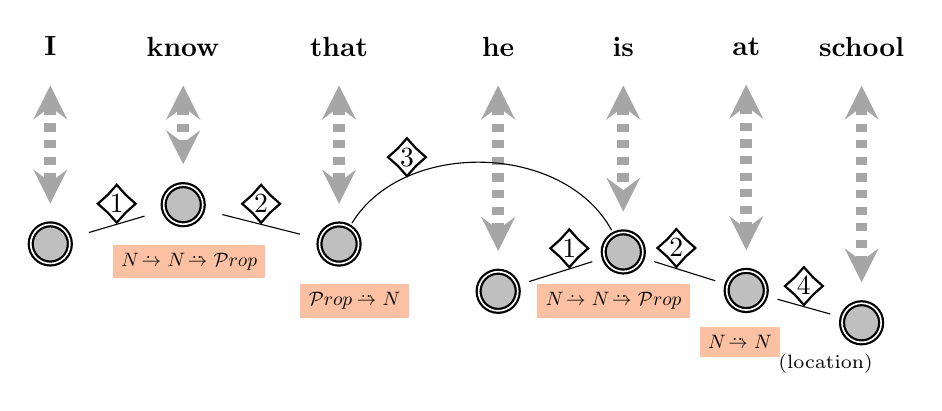
\begin{tikzpicture}

%\draw

%\node [s1] at (0,0) {Student};

\node (I) at (1,1) {\textbf{I}};
\node (know) [right=9mm of I] {\textbf{know}};
\node (that) [right=9mm of know] {\textbf{that}};
\node (he) [right=12mm of that] {\textbf{he}};
\node (is) [right=10mm of he] {\textbf{is}};
\node (at) [right=10mm of is] {\textbf{at}};
\node (school) [right=5mm of at] {\textbf{school}};


\node (IRep) [double,draw=black,shape=circle,thick,fill=gray!50,inner sep=.5em,below=2cm of I] {};
\node (knowRep) [double,draw=black,shape=circle,thick,fill=gray!50,inner sep=.5em,below=1.5cm of know] {};
\node (thatRep) [double,draw=black,shape=circle,thick,fill=gray!50,inner sep=.5em,below=2cm of that] {};
\node (heRep) [double,draw=black,shape=circle,thick,fill=gray!50,inner sep=.5em,below=2.6cm of he] {};
\node (isRep) [double,draw=black,shape=circle,thick,fill=gray!50,inner sep=.5em,below=2.1cm of is] {};
\node (atRep) [double,draw=black,shape=circle,thick,fill=gray!50,inner sep=.5em,below=2.6cm of at] {};
\node (schoolRep) [double,draw=black,shape=circle,thick,fill=gray!50,inner sep=.5em,below=3cm of school] {};

\node (knowRepType) [below right = .2cm and -1.2cm of knowRep] 
 {\colorbox{yellow!20!red!30}{\scalebox{.7}{\NNtoProp}}}; 

\node (thatType) [below right = .2cm and -.8cm of thatRep] 
{\colorbox{yellow!20!red!30}{\scalebox{.7}{\PropToN}}}; 

\node (isRepType) [below right = .1cm and -1.4cm of isRep] 
{\colorbox{yellow!20!red!30}{\scalebox{.7}{\NNtoProp}}}; 

\node (atRepType) [below right = .15cm and -.9cm of atRep] 
{\colorbox{yellow!20!red!30}{\scalebox{.7}{\NtoN}}
}; 

\node (atRepTypeNote) [below right = .5cm and .1cm of atRep] {
	\footnotesize{(location)}
}; 


\draw [ |-,-|, <->, line width = .8mm, draw=gray!70, 
 dashed, double equal sign distance, >= stealth, shorten <= .25cm, shorten >= .25cm ]
 (I) to (IRep);

\draw [ |-,-|, <->, line width = .8mm, draw=gray!70, 
 dashed, double equal sign distance, >= stealth, shorten <= .25cm, shorten >= .25cm ]
(know) to (knowRep);
 
\draw [ |-,-|, <->, line width = .8mm, draw=gray!70,  
 dashed, double equal sign distance, >= stealth, shorten <= .25cm, shorten >= .25cm ]
(that) to (thatRep);

\draw [ |-,-|, <->, line width = .8mm, draw=gray!70, 
 dashed, double equal sign distance, >= stealth, shorten <= .25cm, shorten >= .25cm ]
(he) to (heRep);
 
\draw [ |-,-|, <->, line width = .8mm, draw=gray!70, 
dashed, double equal sign distance, >= stealth, shorten <= .25cm, shorten >= .25cm ]
(is) to (isRep);

\draw [ |-,-|, <->, line width = .8mm, draw=gray!70,  
dashed, double equal sign distance, >= stealth, shorten <= .25cm, shorten >= .25cm ]
(at) to (atRep);

\draw [ |-,-|, <->, line width = .8mm, draw=gray!70, 
dashed, double equal sign distance, >= stealth, shorten <= .25cm, shorten >= .25cm ]
(school) to (schoolRep);
 
 
\draw [shorten <= .25cm, shorten >= .25cm ] 
(knowRep) to node [draw=black,shape = star,star points=4,thick,inner sep = 0mm, above] {1} (IRep);

\draw [shorten <= .25cm, shorten >= .25cm ] 
(knowRep) to node [draw=black,shape = star,star points=4,thick,inner sep = 0mm,above] {2} (thatRep);

\draw [shorten <= .05cm, shorten >= .05cm, bend left=60] 
(thatRep) to node [draw=black,shape = star,star points=4,thick,inner sep = 0mm,above, 
near start] {3} (isRep);


\draw [shorten <= .15cm, shorten >= .15cm ] 
(isRep) to node [draw=black,shape = star,star points=4,thick,inner sep = 0mm,
 above, pos=0.4] {1} (heRep);

\draw [shorten <= .15cm, shorten >= .15cm ] 
(isRep) to node [draw=black,shape = star,star points=4,thick,inner sep = 0mm,above, 
 pos=0.4] {2} (atRep);

\draw [shorten <= .15cm, shorten >= .15cm ] 
(atRep) to node [draw=black,shape = star,star points=4,thick,inner sep = 0mm,above] {4} (schoolRep);


%\draw [shorten <= .25cm, shorten >= .25cm ] 
%(s1Rep) to node [draw=black,shape = star,star points=4,thick,inner sep = 0mm, below] {2} (s2Rep);

%\draw [shorten <= .5cm, shorten >= .5cm ] 
%(afterRep) edge [bend left=20,looseness=1] node [draw=black,shape = star,star points=4,thick,inner sep = 0mm, 
% above, near end ] {3} (complainedRep);

%\node (frameTopLeft) [below left = 1.5cm and -.65 cm of s1] {};
%\node (frameBottomLeft) [below = 2.5cm of frameTopLeft] {};
%\node (frameBottomRight) [right = 3.95cm of frameBottomLeft] {};
%\node (frameTopRight) [above = 2.5cm of frameBottomRight] {};

%\draw [shorten <= 0.15cm, shorten >= 0.15cm ] 
%(frameTopLeft) edge [bend right=30,looseness=1] (frameBottomLeft);

%\draw [shorten <= 0.15cm, shorten >= 0.15cm ] 
%(frameBottomLeft) edge [bend right=30,looseness=1] (frameBottomRight);

%\draw [shorten <= 0.15cm, shorten >= 0.15cm ] 
%(frameBottomRight) edge [bend right=30,looseness=1] (frameTopRight);

%\draw [shorten <= 0.15cm, shorten >= 0.15cm ] 
%(frameTopRight) edge [bend right=30,looseness=1]
%node [draw=black,shape = regular polygon,regular polygon sides=3,thick,inner sep = .2mm, 
%above, near start, shape border rotate = 180] {4} (frameTopLeft);


%node [draw=black,shape = star,star points=4,thick,inner sep = 0mm, above, 
%bend left=100,looseness=3] {3}

%;


\end{tikzpicture}
\end{minipage}

\hspace{0.1\textwidth}
\begin{minipage}{0.8\textwidth}
		\renewcommand{\labelitemi}{$\blacklozenge$}
	
\begin{itemize}\setlength\itemsep{-.3em}
\item 1 \hspace{12pt}  Verb's subject argument
\item 2 \hspace{12pt}  Verb's direct object argument
\item 3 \hspace{12pt}  Propositional \q{packaging} (\q{typed} as {}\PropToN{})
\item 4 \hspace{12pt}  Locative auxiliary link \\
(may be typed as converting nouns to place-designations) 
\end{itemize}
\end{minipage}
\end{figure*}  If these 
requirements are seen as more syntactic, so qualities are incorporated into 
data like Part of Speech (say, a noun designating something with propositional attitudes 
being a subtype of of a generic \N{} type), then we are more likely to analyze 
violations as simply incorrect (recall \q{The tree wants to run away from the dog}
\mdash{} ungrammatical or just somehow \q{exotic}?).  
Some examples suggest less incorrectness as clever or poetic usage \mdash{} so a 
richer analysis may recognize expressions as type- and link-wise acceptable, but 
showing incongruities (which is not the same as impropriety) 
at a more fine-grained type level.  That \i{to want} takes a subject 
\i{associated} with sentience does not force type annotations to inscribe this 
in grammatic or lexical laws; instead, these associations can be 
introduced as potential \q{side effects}, \i{triggering} re-associations 
such as forcing hearers to ascribe sentience to something (like a tree) where 
such ascription is not instinctive.  The type effect in this case lies more 
at the conceptual level, the language-user sifting conceptual 
backgrounds to find a configuration proper to the type requirements (in what 
sense can a tree \q{want} something?).  In this \q{tree} case we probably 
appeal to concepts of \q{as if}: if the tree \i{were} sentient, it 
would be nervous of the dog sniffing around \mdash{} a humorous way of calling 
attention to the dog's actions (obliquely maybe alluding to people's background 
knowledge that dogs sometimes do things, like pee, in inconvenient 
places, from humans' perspectives).  
}
\p{In brief, it is certainly possible \mdash{} though by no means mandatory \mdash{} to model 
type requirements with greater flexibility at a provisional grammatical layer, 
and then narrow in on subtypes or extra accumulations of qualifications on 
type-instances in a transition from grammar to semantics.  Perhaps cognitive 
schema occupy an intermediary role: progressing from basic recognition of 
grammaticality, through cognitive schema, to conceptual framing, with type 
machinery capturing some of the thought-processes at each \q{step} 
(not that such \q{steps} are necessarily in a temporal sequence).  The basic 
verb-subject-direct object articulation sets up an underlying cognitive 
attitude (represented by a basic type-framing of verb, noun, and proposition, 
like the \VisNNtoProp{} signature).  Cognitive ascriptions fill this out 
by adding detail to the broader-hewed typing, associating sentience with the 
subject and propositionality with the object (sub- or higher-order typing 
modeling this stage).  And how the actual lexical choices fit these cognitive 
expectations \mdash{} I call them cognitive because they are intrinsically tied 
to structurational schema in the type, morphology, and word-order givens 
in the encountered language \mdash{} compels conversants to dip into background 
beliefs, finding concepts for the signified meanings that hew to the 
intermediary cognitive manipulations (finding ways to conceptualize the 
subject as sentient, for example).  This also has a potential type model, 
perhaps as forcing a type conversion from a lexical element which does 
not ordinarily fit the required framing (such as giving inanimate things 
some fashion of sentience).  Type theory 
can give a window onto unfolding intellection at these multiple stages, 
although we need not conclude that the mind subconsciously doing this thinking 
mimics a computer that churns through type transformations mechanically and exactly.
}
\p{I envision the unfolding that I have just sketched out as something Phenomenological 
\mdash{} it arises from a unified and subjective consciousness, one marked by 
embodied personal identity and social situation.  If there are structural stases 
that can be found in this temporality of experience, these are not constitutive 
of conscious reality but a mesh of rationality that supports it, like the veins in 
a leaf.  Stuctural configurations can be lifted from language insofar as it is a 
conscious, formally governed activity, and lifted from the ambient situations which 
lend language context and meaning intents.  So any analytic emphasis on  
structural fixpoints threaded through the lived temporality of consciousness is an 
abstraction, but one that is deliberate and necessary if we want to make scientific 
or in any other manner disputatable claims about how language and congition works.  
In that spirit, then, I will try to condense the three \q{layers} of unfolding 
understanding, which as I have sketched them are posited in the metaphysical order 
of temporal experience \mdash{} \q{unfolding} in likely overlapping, blending ways 
\mdash{} I will \q{read into} them a more static and logically stacked meta-structure.  
Where I have sketched three layers or stages of unfolding language understanding, 
I will transition to proposing three \q{tiers} of language organization, in particular 
three levels where type-theoretic models can be applied.
}

\subsection{Three tiers of linguistic type theory}
\p{By three \q{tiers} of linguistic organization, I am thinking of
different levels of granularity, distinguished by relative scales of
resolution, amongst the semantic implications of
putative type representations for linguistic phenomena.
Type-related observations can be grouped (not necessarily
exclusively or exhaustively) into those I will call
\i{functional} \mdash{} relating mostly to Parts of Speech and the functional treatment
of phrases as applicative structures; \i{Ontological} \mdash{} engaged with
existential/experiential qualities like sentient/nonsentient, rigid/nonrigid, and
others I have discussed; and \i{Lexical} \mdash{} related to lexemes and word-senses.
The lexical level can include  \q{microclassification}, or
gathering nouns and verbs by the auxiliary prepositions they allow and
constructions they participate in (such as, different cases), and
especially how through this they compel various spatial and
force-dynamic readings; their morphosyntactic resources for describing states
of affairs; and, within semantics, when we look toward even more fine-grained classifications
of particular word-senses, to reason through contrasts in usage.\footnote{So, conceiving microclasses similar in spirit to Steven Pinker in
Chapter 2 of \cite{Pinker}, though I'm not committing to using the
term only in the way Pinker uses it.  Cf. also \cite{AnneVilnat}, which
combines a microclass theory I find reminiscent of \i{The Stuff of Thought} with
formal strategies like Unification Grammar.
}  Microclasses can point out similarities
in mental \q{pictures} that explain words' similar behaviors, or
study why different senses of one word succeed or fail to be acceptable in particular phrases.
There are \i{stains all over the tablecloth} and \i{paint splattered all over the tablecloth},
but not (or not as readily) \i{dishes all over the tablecloth}.  While \q{stains} is count-plural and
\q{paint} is mass-aggregate, they work in similar phrase-structures because both
imply extended but not rigid spatial presence; whereas \q{dishes} can work for
this schema only by mentally adjusting to that perspective, spatial construal shifting
from visual/perceptual to practical/operational (we might think of dishes \q{all over} the
tablecloth if we have the chore of clearing them).  Such observations support
microclassification of nouns (and verbs, etc.) via Ontological and
spatial/dynamic/configuration criteria.
}
\p{Type-theoretic semantics can also apply Ontological tropes to unpack the overlapping mesh of word-senses,
like \i{material object} or \i{place} or \i{institution}.
This mode of analysis is especially well illustrated when competing senses
collide in the same sentence.  Slightly modifying two examples:\footnote{\cite[p. 40]{ChatzikyriakidisLuo} (former) and
\cite[p. 4]{MeryMootRetore} (latter).
}
\begin{sentenceList}\sentenceItem{} The newspaper you are reading is being sued.
\sentenceItem{} Liverpool, an important harbor, built new docks.
\end{sentenceList}
Both have a mid-sentence shift between senses, which is analyzed
in terms of \q{type coercions}.  The interesting detail of this treatment
is how it correctly predicts that such coercions are not guaranteed to
be accepted \mdash{} \i{the newspaper fired the reporter and fell off
the table}; \i{Liverpool beat Chelesea and built new docks}
(again, slightly modifying the counter-examples).  Type coercions are
\i{possible} but not \i{inevitable}.  Certain senses \q{block} certain coercions
\mdash{} that is, certain sense combinations, or juxtapositions, are disallowed.
These preliminary, motivating analyses carry to more
complex and higher-scale types, like plurals (the plural of a type-coercion
works as a type-coercion of the plural, so to speak).
As it becomes structurally established that type rules at the
simpler levels have correspondents at more complex levels, the use of
type notions \i{per se} (rather than just \q{word senses} or other
classifications) becomes more well-motivated.
}
\p{Clearly, for example,
only certain kinds of agents may have beliefs or desires, so
attributing mental states forces us to conceive of their referents
in those terms (\i{Liverpool wants to sign a talented young striker}).
This \i{can} be analyzed as \q{type coercions}; but the type-theoretic machinery should contribute
more than just obliquely stating linguistic wisdom, such as
maintaining consistent conceptual frames or joining only suitably
related word senses.  The sense of \i{sign} as in \q{employ to play on
a sports team} can only be linked to a sense of Liverpool as the
Football Club; or \i{fire} as in
\q{relieve from duty} is only compatible with newspapers as
institutions.  These dicta can be expressed in multiple ways.
But the propagation of classifications
(like \q{inanimate objects} compared to
\q{mental agents}) through complex type structures lends credence to the
notion that type-theoretic perspectives are more than just an expository tool;
they provide an analytic framework which integrates grammar and semantics, and
various scales of linguistic structuration.
For instance, we are prepared to accept some examples of dual-framing
or frame-switching, like thinking of a newspaper as a physical object and a city government
(but we reject other cases, like \q{Liverpool voted in a new city government and signed a
new striker} \mdash{} purporting to switch from the city to the Football Club).  The rules for
such juxtapositions appear to reveal a system of types with some parallels to
those in formal settings, like computer languages.
}
\p{In short, \q{Ontological} types like \i{institution} or \i{place} serve in some
examples to partition senses of one multi-faceted word.  Here they reveal
similar cognitive dynamics to reframing-examples like \i{to the press}, where
Ontological criteria (like reading something as a place) are triggered by
phrase-scale structure.  But there are also interesting contrasts:
the \i{newspaper} and \i{Liverpool} examples
imply that some words have multiple framings which are well-conventionalized;
newspaper-as-institution feels less idiomatic and metaphorical than
press-as-place.  So these examples suggest two \q{axes} of variation.
First, whether the proper Ontological framing follows from other word-choices
(like \q{fire} in \i{the newspaper fired the reporter}, which has
its own semantic needs), or from morphosyntax
(like the locative in \i{to the press}); and, second, whether triggered framings work
by selecting from established word senses or by something more metaphorical.
Metaphors like \i{to the press} do have an element of standardization;
but apparently not so much so to be distinct senses: note how \i{the press} as metaphorical place
does not work in general: \qmarkdubious{}\i{at the press}, \qmarkdubious{}\i{near the press}
(but \i{at the newspaper}, \i{near the newspaper}
\mdash{} imagine two journalists meeeting outside the paper's offices \mdash{} sound quite reasonable).
}
\p{The \q{type coercion} analysis works for mid-sentence frame-shifts; but other
examples suggest a more gradual conceptual \q{blending}.  For example, the
place/institution dynamic is particularly significant for \i{restaurant}
(whose spatial location is, more so, an intrinsic part of its
identity).  Being a \i{place} implies both location and extension; most places are not single
points but have an inside where particular kinds of things happen.  I am not convinced
that restaurant as place and as institution are separate word senses; perhaps, instead,
conversations can emphasize one aspect or another, non-exclusively.  As I have argued,
we need not incorporate all framing effects via \q{subtypes} (restaurant as either
subtype of hypothetical \q{types of all} places or institutions, respectively).  But
\q{placehood}, the Ontological quality of being a place \mdash{} or analogously being
a social institution \mdash{} identify associations that factor into cognitive frames; types
can then be augmented with criteria of tolerating or requiring one association or another.
So if \q{restaurant} is a type, one of its properties is an institutionality that \i{may}
be associated with its instances.  In conversation,
a restaurant may be talked about as a business or community, foregrounding this
dimension.  Or (like in asking for directions) its spatial dimension may be foregrounded.
The availability of these foregroundings is a feature of a hypothetical restaurant type,
whether or not these phenomena are modeled by subtyping or something more sophisticated.
The \q{newspaper} examples suggest how Ontological considerations
clearly partition distinct senses marked by properties like objecthood or
institutionality (respectively).  For \q{newspaper} the dimensions are less available for
foregrounding from a blended construal, than \q{unblended} by conventional usage; that
is why reframings evince a type \i{coercion} and not a gentler shift of emphasis.
The example of \i{restaurant}, in contrast, shows that competing routes for
cognitive framing need not solidify into competing senses, though they trace
various paths which dialogs may follow.
But both kinds of examples put into evidence an underlying
cognitive-Ontological dynamic which has potential type-oriented models.
}
\p{At the most general level \mdash{} what I called \i{functional} type modeling \mdash{} a type
system recognizes initially only the grammatical backbone of expressions, and
then further type nuances can be seen as shadings and interpretations which add substance
to the syntactic form.  So in type-theoretical analysis at this more grammatic level,
to which I now turn, we can still keep the more fine-grained theory in mind:
the relation of syntax to semantics is like the relation of a spine to its flesh,
which is a somewhat different paradigm than treating syntax as a logical or temporal
stage of processing.  Instead of a step-by-step algorithm where grammatical parsing
is followed by semantic interpretation, the syntax/semantics interface can be seen
as more analogous to stimulus-and-response: observation that a certain grammatic
configuration appears to hold, in the present langauge artifact, triggers a marshaling
of conceptual and cognitive resources so that the syntactic backbone can be filled in.
Perhaps a useful metaphor is grammar as gravitation, or the structure of a gravitational
field, and semantics is like the accretion of matter through the interplay of multiple
gravitational centers and orbits.  For this analogy, imagine typed lambda
reductions like \PropToNYieldsN{} taking the place of gravitational equations;
and sentences' grammatic spine taking the place of curvature pulling mass into a planetary center.
}
\p{Parts of speech have \q{type signatures}
notionally similar to the signatures of function types in programming languages: a verb
needing a direct object, for example, \q{transforms} two nouns (Subject and Object)
to a proposition, which I have been notatating with something like \NNtoS{}.
At the most basic level, the relation of Parts of Speech to \q{type signatures}
seems little more than notational variants of conventional linguistic
wisdom like a sentence requiring a noun and a verb (\SeqNPplVP{}).
Even at this level, however, type-theoretic intuitions
offer techniques for making sense of more complex, layered sentences,
where integrating link and phrase structures can be complex.
Even the most broadly scoped analysis of type signatures, dealing only with
generic Parts of Speech like nouns and verbs, can lead to surprising
complications.  One example I have alluded to several times, and will return to shortly:
the problem of applying Dependency Grammar where phrases do not seem
to have an obviously \q{most significant} word for linkage with other phrases.
}
\p{A tendency in both dependency and phrase-oriented perspectives is to define
structures around the most \q{semantically significant} words \mdash{} so that a phrase
like \q{many students} becomes in some sense collapsible to its semantic
core, \q{students}.  Some of my earlier examples, however, argued that
phrases cannot just be studied as replacements for semantic units.  Incorporating
type theory, we can instead model phrases through the perspective of
type signatures: given Part of Speech annotations for phrasal units and then for
some of their parts, the signatures of other parts, like verbs or adjectives
linked to nouns, or adverbs linked to verbs, tend to follow automatically.
A successful analysis yields a formal tree, where if (in an act of semantic
abstraction) words are replaced by their types, the \q{root} type is something like
\Prop{} and the rest of a tree is formally a reducible structure in
Typed Lambda Calculus: \NNtoProp{} \q{collapses} to \Prop{}, \ProptoN{} collapses
to \N{}, and so forth, with the tree \q{folding inward} like a
fan until only the root remains \mdash{} though a more subtle analysis would
replace the single \Prop{} type with variants that recognize different
forms of speech acts, like questions and commands.  In Figure ~\ref{fig:Iknow},
this can be seen via the type annotations: from right to left \NtoN{} yields the
\N{} as second argument for \i{is}, which in turn yields a \Prop{} that is mapped
(by \i{that}) to \N{}, finally becoming the second argument to \i{know}.  This calculation
only considers the most coarse-grained classification (noun, verb, proposition) \mdash{} as I
have emphasized, a purely formal reduction can introduce finer-grained grammatical or
lexico-semantic classes (like \i{at} needing an \q{argument} which is somehow an expression
of place \mdash{} or time, as in \i{at noon}).  Just as useful, however, may be analyses
which leave the formal type scaffolding at a very basic level and introduce
finer type or type-instance qualifications at a separate stage.
}
\p{In either case, Parts of Speech are modeled as (somehow analogous to) functions, but the important
analogy is that they have \i{type signatures} which formally resemble functions'.
Phrases are modeled via a \q{function-like} Part of Speech along with one or more
additional words whose own types match its signature; the type calculations
\q{collapsing} these phrases can mimic semantic simplifications
like \q{many students} to \q{students}, but here the theory is explicit
that the simplification is grammatic and not semantic: the collapse
is acknowledged at the level of \i{types}, not \i{meanings}.  In addition,
tree structures can be modeled purely in terms of inter-word relations
(this is an example of embedding lambda calculii in process algebras),
so a type-summary of a sentence's phrase structure can be notated and
analyzed without leaving the Link Grammar paradigm.
}
\p{As a concrete example, in the case of \q{many students},
both \q{students} and the semantic role of
the phrase are nouns (count-plural nouns, for where that's relevant).  Accordingly,
\q{many} has a signature \NtoN{} (or \NpltoNpl{}, dependending on how
narrowly we want to notate the types in context).
Once we assign types and signatures to all words in a sentence, we can also see a
natural hierarchy resembling an expression in typed lambda calculus, where some words
appear as \q{functions} and others as \q{arguments}.  Often the less
semantically significant words appear as \q{higher} in the structure,
because they serve to modify and lend detail to more significant words.
The kind of structure or \q{Charpente} which falls out of a sentence \mdash{}
adopting a term from \Tesniere{} (cf. \cite[p. 181]{ElkeTeich}) \mdash{} is typically different from a link-grammar
\q{linkage}, although the two structures can be usefully combined.
}
\p{To return to the example of \q{Student after student}, where designating
one word to \q{represent} the phrase seemed arbitrary, we can analyze the
situation via type-signatures.  I have teased a proposed solution repeatedly;
here's what I had in mind.  Insofar as \i{after} is the only non-noun,
the natural conclusion is that \q{after} should be typed \NNtoN{}
(which implies that \q{after} is analogous to the \q{functional} position, and
in a lambda-calculus style reconstruction would be considered the \q{head}
\mdash{} Figure ~\ref{fig:ESA} is an example of how
the sentence could be annotated, for sake of discussion).
This particular idiom depends however
on the two constituent nouns being the same word (a pattern I've also alluded to with
idioms like \i{time after time}), which can be accommodated by invoking the (computationally rather complex
and topical) concept of \i{dependent types} \cite{BernardyEtAl}, \cite{TanakaEtAl}
\mdash{} in other words the parameters
for \i{after} are a dependent type pair satisfied by an identity comparison between
the two nouns.  The signature for \q{after} has this added complication, but
the nuances of this example can still be accommodated within the overall
architecture of type theory.  I would pair this argument with my earlier
analysis of \q{many} variations which suggested how apparent complications
can be accommodated largely within the extant theoretical resources of
Link Grammar, and in combination suggest that the union of Link Grammar
with Type-Theoretic Semantics seems poised to accommodate many
complex real-world linguistic cases with a coherent abstract perspective.
}
\p{Consider alternatives for \q{many students}.  The phrase as
written suggests a type signature (with \q{many} as the \q{function-like} or
derivative type) \NpltoNpl{}, yielding a syntactic interpretation of the phrase; this
interpretation also suggests a semantic progression, an accretion of intended detail.
From \i{students} to \i{many students} is a conversion between two plural nouns
(at the level of concepts and semantic roles); but it also implies relative size,
so it implies some \i{other} plural, some still larger group of students from which
\q{many} are selected.  While rather abstract and formal, the \NpltoNpl{} representation
points toward a more cognitive grounding which considers this \q{function} as a form
of thought-operation; a refinement of a situational model, descriptive resolution,
and so forth.  If we are prepared to accept a cognitive underpinning to semantic
classification, we can make the intuition of part of speech signatures as \q{functions}
more concrete: in response to what \q{many} (for example) is a function \i{of},
we can say a function of propositional attitude, cognitive schema, or attentional
focus.  The schema which usefully captures the sense and picture of \q{students} is
distinct (but arguably a variation on) that for \q{many students}, and there is a
\q{mental operation} triggered by the \q{many students} construction which
\q{maps} the first to the second.  Similarly, \q{student after student} triggers a
\q{scheme evolution} which involves a more explicit temporal unfolding
(in contrast to how \q{many students} instead involves a more explicit
quantitative \i{many/all} relation).  What these examples show is that
associating parts of speech with type signatures is not just a formal
fiat, which \q{works} representationally but does not necessarily capture
deeper patterns of meaning.  Instead, I would argue, type signatures
and their resonance into linkage acceptability structures
(like singular/plural and mass/count agreement) \i{point toward} the
effects of cognitive schema on what we consider meaningful.
}
\p{In \i{Student after student came out against the proposal},
to \i{come out}, for/against, lies in the semantic frame of attitude and expression
(it requires a mental agent, for example), but its reception
carries a trace of spatial form: to come out \i{to} a public place, to
go on record with an opinion (a similar dynamic applies to the idiomatic
\q{come out} to mean, for someone gay or lesbian, \q{come out of the closet}
\mdash{} in that idiom the spatial figure is explicit but metaphorical).  Usually
\q{come out [for/against]}, in the context of a policy or idea, is similarly
metaphorical.  But the concrete spatial interpretation remains latent, as a kind
of residue on even this abstract rendition, and there sustains a chance that this
undercurrent will actually figure in conversants' mutual understanding \mdash{} if
there were not just columns being written and opinions voiced but demonstrations
on the quad.  The spatial undercurrent is poised to emerge
as more literal, should the context warrant.  However literally or metaphorically
the \q{space} of the cognitive \q{coming out} is
understood, however explicit or latent its cogitative figuration,
is not something internal to the language; it is a potentiality which
will present in different ways in different circumstances.  This is not to say that
it is something apart from linguistic meaning, but it shows how linguistic meaning
lies neither in abstract structure alone, nor contextual pragmatics, but in their cross-reference.
}
\subsection{Levels of formalization}
\p{Of the three type levels I have proposed, the \q{functional} level is the most
quasi-mathematical; for other levels, formal type theory may provide interpretive
tools and methodological guides, but formally representable framings and
transformations may be only approximations of how people actually think, while
they are understanding language.  From this perspective, we are left with the
metatheoretical question of clarifying how different kinds of analyses, which
put different degrees of weight on formal or on interpretive argumentational,
are to be joined in overarching theories.  In particular, are the
linguistic phenomena which seem to demand more \q{interpretive} treatment actually
beyond formalization, or is it just impractical (but possible in theory) to provide
formal analysis of each individual case-study, each real-world language formation?
Is Natural Language actually no less formal than (for example) computer programming
languages, except that the former have a much larger set of semantic and syntactic
rules such that any analysis can uncover them only partially?  Or is any rule-based
model of language, no matter how complete, necessarily partial relative to real language?
}
\p{Computer languages are a good case-study in what I might call \q{semiotic computability}.
This designates the question of whether the
operations of sign-systems \mdash{} how sign-users express intentions by forming or modifying
structured networks of signs that explicitly exhibit or are understood to have been
formed according to collectively recognized signifying rules \mdash{} can be modeled,
at least to some substantial degree, by computable algorithms.  Our
notion of computation can be based on modern computer code, not just academic
topics like pure functions: the behavior of computing systems
where many functions run concurrently, with possible side-effects, is often
non-computable via static analysis; such systems can only be understood by
actually running them.  Nevertheless the capabilities of software programmed
in modern languages certainly deserve to be characterized as \q{computable}
behaviors.  A single function, which embodies a computable
calculation, may be part of a process space whose evolution through
time is nondeterministic, and computing environments which employ
functional side-effects are difficult or impossible to evaluate in the abstract.
I use \q{computability} therefore in this wider sense: operationally implementable
according to theories underlying mainstream programming languages, which is
conceptually (if perhaps not mathematically) distinct from \q{computability} in
subjects like algorithm analysis.
}
\p{Natural Langauge Processing, working with human languages from a computing platform,
is then a step further, continuing beyond logico-mathematic abstractions and toward
empirical language-use.  We can consider at what point formal and computational methods reach a limit,
beyond which they fail to capture
the richess and expressiveness of Natural Language, or whether this limit itself
is an illusion \mdash{} whether even fully human
language competence is (perhaps in principle if not in practice) no less reducible
to formalizable patterns.  Using the wording I just proposed, we can speculate on
whether all language is \q{semiotically computable} or whether language merely
depends on faculties which in some neurological and/or presentational sense are
\q{computable} in those terms \mdash{} faculties that, measured against linguistic fluency,
are necessary but not sufficient.
Whatever one's beliefs on this last question,
a progression of subdisciplines \mdash{} from formal-logical semantics through programming
langauges and computational Natural Langauge Processing \mdash{} is a reasonable
scaffolding for a universe of formal methods that can build up, by progressive theoretical
sophistication or assembly of distinct analyses which piece together jigsaw-like, to model
real-world language understanding.  Perhaps real language is an \q{emergent property} of
many distinct algorithms that run and combine in the mind; or perhaps the relevant
algorithms are a precondition, presenting cognition with essential signifying givens
but fleshed out in other, more holistic ways, as we become conscious of language not
just as a formal system but an interactive social reality.
}
\p{I have sketched a similar theoretical progression, starting with a theory of
grammar (Link Grammar), transitioning to a form of semantics (a type-theoretic semantics
defining type hierarchies and signatures over linkage graphs), and finally proposing a
cognitive interpretation of the resulting semantics.  I will refer to this
\i{interpretation} as  \q{Cognitive State Semantics}, meaning that such a theory
adopts its \i{formal} structures from Link Grammar and type-theory but also attempts
to \i{motivate} these structures by appeal to cognitive considerations.  Both Link Grammar
(through its specific Category of labeled graphs modeling sentence linkage-structures) and
Type-Theoretic Semantics work with rigorous, algebraically formal models satisfying criteria
I referenced at the end of the last section: translation of language content into these
formats and subsequent review or transformation of the target structures can be programmed
as a purely mechnical space of operations.
}
\p{By itself, the superposition of
type-theoretic semantics on link-grammar graphs does not cross a hypothetical \q{barrier} between
the formal and the cognitive.  But I intend here to suggest a cognitive \i{interpretation}
for the formal structures; that they represent an outline of cognitive schema, or progressions,
or represent linguistic \q{triggers} that a cognitive language ability (taking language
as part of an environing world and produced by others, in rule-bound social situations,
to communicate ideas and sentiments) responds to.  This range of interpretations is
deliberately open-ended: we can say that a formal infrastructure grounds the cognitive
reception of language givens, without arguing specifically that formal structures identified
in language therefore model cognitive operations directly, or that these are instead
patterns identified in language that trigger a cognitive response, or any other
paradigm for mapping cognition as process and activity to language structure as model and
prototype.  Leaving these options open, however, I will focus in the remainder of this
paper on one interpretation, considering formal structures as \q{triggers} which
get absorbed into language understanding via observatory propensities: as language
users (on this proposal) we are disposed to identify certain formal structurations
operating in language as we encounter it, and respond to these observations by building
or refining mental models of the situations and signifying intentions we believe have been
implied by the discourse, in evolving and intersubjective dialogic settings that involve
joint practical activity as well as communication.
}
\p{In this sense, I believe natural language reveals mutually-modifying juxtapositions
of concepts whose full semantic effects
are probably non-computable: I would work on the assumption that language
\i{as a whole} and as human social phenomena is not \q{computable} in a
semiotic sense, or any related practical sense (although
I make no metaphysical claims about the \q{abstract} computability of mental
processes merely by virtue of their neurophysical materiality).
The aforementioned \q{linguistic side effects} can be \i{modeled} by tracing our reception
of linguistic meaning through syntactic and semantic formations, like Link Grammar
and Type Theory, but I argue for such models not as models \i{of} cognitive processes,
but rather models of \i{observations} which trigger cognitive follow-up.  Even if we
believe in and practice a rigorous formalization of morphosyntactic structure,
where the \i{pattern} of conceptual \q{side-effects} can be seen as
unfolding in algorithmic ways, the cognitive \i{details} of these
effects are too situational, and phenomenologically rich, for
computability as ordinarily understood.  But the formal structure is
not wholly irrelevant: to call up nuanced cognitive schema
\mdash{} or so I submit for consideration \mdash{} may not be possible without
algorithmically reproducible lexicosemantic and morphosyntactic triggers,
at least modulo some approximation.  A (perhaps non-computable) space
of cognitive schema may be projected onto a (perhaps computable)
set of affiliated morphological patterns, using notations like
link-grammar pairs and type signatures to catalog them.  For example, there may be a non-computable
expanse of possible construals of pluralization; but any such construal,
in context, is called into focus in conversants' minds by morphosyntactic
invitations, by speakers' choices of, say, \mbox{\NSingToNPl{}}-pattern
phrases.  The important balance is to take formalization as far as is reasonable
without being seduced into logico-symbolic reductionism \mdash{} a
methodological pas de deux I will explore further in the next, concluding section.
}
\p{Any word or usage invites various facets to either
emphasize or deemphasize, and these subsumed concepts or foci are
latent in potential meanings, brought into linguistic space
by the play of differentiation \footnote{Alluding, in part, to Sausurrean \q{system of differences}
\cite[p. 15]{EfePeker} \mdash{} to choose a reference which introduces
Sausurre in a rather unexpected context.
}
: \i{baked}, not \i{made}; \i{flew}, not \i{traveled};
\i{spill}, not \i{pour}.
These under-currents of subsidiary concepts and foci are selectively hooked onto by
morphosyntactic selection, so in analyzing phrase
structure we also have to consider how using syntax
which constructs a given structure also brings to the forefront certain
nested concepts and construals, which are latent in word-sense options;
in the topos of lexicosemantic possibilia.
}
\p{So, any talk about \q{side effects} of morphosyntactic functions
\mdash{} mapping verb-space to adjective-space, noun-space to
proposition-space, singularity to plurality, and so forth \mdash{} should consider
a type-theoretic gloss like \NtoN{} as sketching just the motivating
scaffold around an act of cognitive refocusing.  The interesting semantics
lies with \i{how} a sense crosses over, in conversants' minds,
to some other sense or concept, wherein other aspects are foregrounded
\mdash{} for example, within temporal event plurality: multiplicity as
frequency, or episodic distribution relative to some time span;
or suggesting something that is typical
or predominant; or relative count against some other
totality \mdash{} each such refocusing triggered by a phrasal construction
of the form \NtoNpl{} or \mbox{\NpltoNpl{}}.
Or we can map singulars, or count plurals, to mass nouns, and vice-versa (\i{shrubs} become \i{foliage};
\i{water} becomes \i{a glass of water}).
The plural and the singular are a coarse-grained semantic that has not yet arrived as \i{meaning}.
Conceptual spaces guide attention to classes and properties, defining a path of ascending
precision as speakers add descriptive detail;
cognitive construals negotiate relations between different kinds
of aggregates/individuals; individuality, aggregation and multiplicity as phenomena and
disposition.  These construals are practical and embodied, \i{and}
phenomenological \mdash{} they direct attention (\i{qua} transcendental universal of
mentality, if we like), to and fro, but in the course of intersubjective and
goal-driven practical action (and in that sense particular, world-bound, historicized).
}
\p{Given these considerations, I propose a \q{Cognitive State Semantics}
\mdash{} understanding phrase structure in terms of (or analogous to) functional effects
(like \cite{ShanThesis}), but cognitive: word and syntax choice effectually
steering cognitive appraisals of jointly experienced situations
in specific directions.  Cognitive State Semantics also has formal implications:
the inner structuration of data \q{spaces},
including unknown and undefined values, and including (side-effects-bearing) function types,
can be understood as dynamic \i{states of knowledge} and their changes, grounding datatype semantics in human
use/interactions.  Linguistically, the \q{effects} of language \q{functions} are
mutations/modifications in cognitive state, respondant to concrete
or abstract scenarios which are topics of dialog.  Sometimes, effects may
tolerate mathematical analysis; but such analytical thematics tend to peter out into the
ambient, chaotic worldliness of human consciousness.
}

%\section{Truth-Theoretic Semantics and Enaction}
\p{Corrolary to the idea that roles often determine 
concepts, is the recognition that 
we tend to logically evaluate situations in 
functional terms, through the lens of what 
we (or any of our peers) are \i{doing}.  
Suppose my friend says this, before and after: 
\begin{sentenceList}\sentenceItem{} Can you put some almond milk in my coffee?
\sentenceItem{} Is there milk in this coffee?
\end{sentenceList}
Between ()and () I do put almond milk in his 
coffee and affirm \q{yes} to ().  I feel it 
proper to read ()'s \q{milk} as really meaning 
\q{almond milk}, in light of ().  Actually 
I should be \i{less} inclined to say \q{yes} 
if (maybe as a prank) someone had instead 
put real (cow) in the coffee.  In responding 
to his question I mentally substitute what 
he almost certainly \i{meant} for how
(taken out of context) () would usually 
be interprted.  In this current 
dialog, the \i{milk} concept not only 
includd vegan milks, apparently, but 
\i{excludes} actual milk.
}
\p{It seems as uf when we are dealing with 
illocutionary force we are obliqued to subject 
what we hear to extra interprtation, rather 
than resting only within \q{literal} meanings 
of sentences, conventionally understood.  
This point is worth emphasizing because it complicates 
are attempts to link illocution with propositional 
content.  Suppose grandma asks me to close the 
kitchen window.  Each of these are plausible and 
basically polite responses: 
\begin{sentenceList}\sentenceItem{} It's not open, but there's still some 
cold air coming through the cracks. 
\sentenceItem{} It's not open, but I closed the window in 
the bedroom.
\sentenceItem{} I can't \mdash{} it's stuck.
\end{sentenceList}
In each case I have not fulfilled her request \visavis{} 
its literal meaning, but I \i{have} acted benevolently 
in terms of conversational maxims.  Many linguists 
seem to analyze hedges like \q{could you please} 
as merely dressing over crude commands: we don't 
want to come across as giving people orders, but 
sometimes we do intend to ask pople to do specific 
things.  As a result, we feel obliged to couch the 
request in conversational gestures that signal 
our awareness of how bald commands may lie outside 
the conversational norms.  These ritualistic 
\q{could you please}-like gestures may have 
metalinguistic content, but \mdash{} so the theory 
goes \mdash{} they do not \i{smantically} alter 
the speech-act's directive nature.
}
\p{The problem with this analysis is that sometimes 
directive and \q{inquisitive} dimensions can 
overlap: 
\begin{sentenceList}\sentenceItem{} Do you have almond milk?
\sentenceItem{} Can you get MsNBC on your TV?
\end{sentenceList}
These \i{can} be read as bare directives, and would 
be interprted as such if the hearer believed the 
speaker already knew that yes, he has almond milk, and yes, 
he gets MsNBC.  They can also be read as bare 
questions with no implicature: maybe fans of 
almond milk and MsNBC endorsing those selections.  
They can \i{also} be read as a mixture of the 
two, as if people expressed themselves like this:
\begin{sentenceList}\sentenceItem{} I think the window is open, can you close it?
\sentenceItem{} I see you have almond milk, can I have some?
\sentenceItem{} If you get MsNBC, can you turn on Rachl Maddow?
\end{sentenceList}
}
\p{I think the mixed case is the most prototypical and pure 
directives or inquiries should be treated as degenerate 
structures whre either directive or inquisitive content 
has dropped out.  After all, even a dictatorial 
command includs the implicit assumption that the order 
both makes sense and is not impossible.  On 
the other hand, we don't ask questions for no 
reason: \q{do you hav almond milk} may be a 
suggestion rather than a request, but it still 
carries an implicature (e.g., that the addressee 
\i{should} get almond milk).   
}
\p{Ordinary requests carry the assumption that addressees 
can follow through without undue inconvenience, 
which includs a package of assumptions about borh 
what is currently the case and what is possible.  
\q{Close the window} only has literal force if the 
window is open.  So when making a request speakers 
have to signal that they recognize the request involves 
certain assumptions and are rational enough to 
accept modifications of these assumptions in 
lieu of literal compliance.  This is why 
interrogative forms liie \q{can you} or 
\q{could you} are both semantically nontrivial 
and metadiscursively polite: they leave open the 
possibility of subsequent discourse framing the original 
request just as a belief-assertion.  Developments 
like \q{can you open the window} \mdash{} \q{no, it's closed} 
are not ruled out.  At the same time, interrogative forms 
connote that the speaker assumes the addressees can 
fulfill the request without great effort: an implicit 
assumption is that they \i{can} and also \i{are 
willing to} satisfy the directive.  This is an 
assumption, not a prsumption: the speaker 
would seem like a bully if he acted as if he 
gave no thought to hid demands being too much 
of and imposition.  This is another rason why requests 
should be framed as question.
}
\p{Sometimes the link between directives and 
belief assertions is made explicit.  A common 
pattern is to use \q{I believe that} as anb
implicature analogous to interrogatives: 
\begin{sentenceList}\sentenceItem{} I believe you have a reservation for Jones?
\sentenceItem{} I believe this is the customer service desk?
\sentenceItem{} I believe we ordered a second basket of garlic bread?
\sentenceItem{} I believe you can help me find a find computer 
acessories in this section?
\end{sentenceList}
These speakers are indirectly signaling what they want 
someone to do by openly stating the requisite 
assumptions \mdash{} \i{I believe you can} in place 
of \i{can you?}.  The implication is that 
such assumptions translate clearly to a 
subsequent course of action \mdash{} the guest who 
\i{does} have that rservation should be checked in; 
the cashier who \i{can} help a customer find 
accessories should do so.  But underlying these 
performances is recognition that 
illocutionary force is tied to background 
assumptions, and conversants are reacting to 
the propositional content of thos assumptions 
as well as the force itself.  If I \i{do} close the 
window I am not only fulfilling 
the request but also confirming that the window 
\i{could} be closed (a piece of information 
that may become relevant in the future).  
}
\p{In sum, when we engage pragmatically with other 
language-users, we tend to do so coopratively, 
sensitive to what they wish to achieve with 
language as well as to the propositional 
details of their discourse.  But this often means 
that I have to interpret propositional 
content in light of contexts and implicatures.  
Note that both of these are possible:
\begin{sentenceList}\sentenceItem{} Do you have any milk?
\sentenceItem{} Yes, we have almond milk.
\sentenceItem{} No, we have almond milk.
\sentenceItem{} Yes \mdash{} actually, we have almond milk.
\sentenceItem{} No, we only have almond milk.
\end{sentenceList}
A request for milk in a vegan restaurant could plausibly be 
interpreted as a request for a vegan milk-substitute.  
So the concept \q{milk} in that context may actually be 
interpreted as the concept \q{vegan milk}.  As Luo 
points out in [], particular concept-maps are 
admissible as in force in specific situations even 
if they deviate noticably from typical usage 
(Luo does not talk about concept \q{maps} but 
about subtyping and various inter-type relations, 
yielding a type-theory of situations I think 
is relevant Conceptual Role theories of situations).  
In any case, responding to the force of speech-acts 
compels me to treat them as not \i{wholly} 
illourionary \mdash{} as in part statements of 
belief (like ordinary assertions).  One reason I need 
to adopt an epistemic (and not just obligatory) 
attitude to illocutionary acts is that I need to 
clarify what meanings the speaker intends, which 
depends on what roles she is assigning to 
constituent concepts.
}
\p{If a diner asks for milk in a vegan restaurant, 
a waiter may plausbily infer that the customer 
believes the restaurant \i{only has} vegan milk, 
so there is no ned to make that explicit; and/or 
she assumes that everyone in the restaurant will hear 
\q{milk} as \q{vegan milk}.  In other words, the 
waiter infers that \q{vegan milk} for her plays the 
same role as \q{milk} for a non-vegan.  This inference 
is not produced by any speech-act subtleties: a related 
inference would be involved in 
\begin{sentenceList}\sentenceItem{} Is there milk in this coffee?
\sentenceItem{} Yes, almond milk.
\end{sentenceList}
Part of reading propositional content is 
syncing our conceptual schemas with our fellow 
conversants.  But the illocutionary 
dimension of a request like \q{can I have some milk?} 
makes this interpretation especially important, 
because the addressee wants to make a good-faoth effort 
to cooperate with the pragmatic intent of the 
spech-act.  But cooperation requires the 
cooperating parties' conceptual schemas to 
be properly aligned.  I therefore have to 
suspend the illocutionary force of a directive 
temporarily and treat it as locutionary 
statement of belief, interpret its apparent 
conceptual undrpinnings in that mode, and 
then add the illocutionary force back in: if I 
brought \i{real} milk to a vegan customer who 
asked for \q{milk} I would be \i{un}-cooprative.
}
\p{The upshot is that conversational implicatures 
help us contextualize the conceptual negotiations 
that guarantee our grasping the correct 
propositional contents, and vice-versa.  This means 
that propositionality is woven throughout both 
assretive and all other mods of language, but it 
also means that propositional content can be 
indecipherable without a detailed picture 
of the current context (including illocutionary 
content).  The proposional content of, 
say, \q{there is milk in this coffee} has to be 
judged sensitive to contexts like \q{milk} 
meaning \q{vegan milk} \mdash{} and this 
propagates from a direct propositional 
to any propositional attitudes which may 
be directed towards it, including requsts like 
\q{plase put milk in this coffee}.
}
\p{Suppose the grandkids close grandma's bedroom window 
when she asks them to close the kitchen window.  
The propositional content at the core of grandma's 
request is that the kitchen window be closed; the 
content attached to it is an unstated belief that 
this window is open.  Thus, the truth-conditions 
satisfying her implicit understanding would be 
that the kitchen window went from being open to being 
closed.  As it happens, that window is already 
closed.  So the truth-conditions that would satisfy 
grandma's initial belief-state do not obtain \mdash{} her 
beliefs are false \mdash{} but the truth conditions satisfying 
her desired result \i{do} obtain.  The window 
\i{is} closed.  Yet the grand kids should not thereby 
assume that her request has been properly responded to; 
it is more polite to guess at the motivation behind 
the request, e.g., thay she felt a draft 
of cold air.  In short, they should look outside 
the truth conditions of her original 
request taken literally, and \i{interpret} 
her requesting, finding different content 
with different truth-conditions that are both consistent 
with fact and address whatever pragmatic goals 
grandma had when making her request.  They might 
infer her goal is to prevent an uncomfortable 
draft, and so a reasonable \q{substitute content} is 
the proposition that \i{some} window is open, 
and they should close \i{that} one. 
}
\p{So the grandkids should reason as if translating 
between these two implied meanings: 
\begin{sentenceList}\sentenceItem{} I believe the kitchen window 
is open \mdash{} please close it!
\sentenceItem{} I believe some window 
is open \mdash{} please close it!
\end{sentenceList}
They have to revise the simplest reading of 
the implicit propositional content of grandma's 
\i{actual} request, because the actual request is 
inconsistent with facts.  In short they 
feel obliged to explore propositional alternatives 
so as to find an alternative, implicit request whose 
propositional content \i{is} consistent with 
fact and also meets the original request's illocutionary 
force cooperatively.  
}
\p{In essence, we need to express a requester's desire as 
itslf, in its totality, a specific propositional content, 
thinking to purselves (or even saying to others) things 
like
\begin{sentenceList}\sentenceItem{} Grandma wants us to close the window.
\sentenceItem{} He wants a bottle opener.
\end{sentenceList}
But to respond politely we need to modify 
the parse of their requests to capture the 
\q{essential} content:
\begin{sentenceList}\sentenceItem{} Grandma wants us to eliminate the cold draft.
\sentenceItem{} He wants something to open that bottle.
\end{sentenceList}
We have to read outside the literal unterpretation 
of what they ar saying.  This re-reading is something 
that may be appropriate to do with respect to 
other forms of speech also: sometimes 
the true gist of what someone wants to communicate 
is not stated directly:
\begin{sentenceList}\sentenceItem{} I think you could do excellent work in 
this class, and I think you are doing pretty well.
\sentenceItem{} I am not going to talk about the refs because 
I don't want to get fined.
\sentenceItem{} If she wants to win the nomination she 
needs to be as charismatic on the campaign trail as 
she was during the debate.
\end{sentenceList}
But our conversational responsibilty to infer 
some unstated content is especially pronounced 
when we are rsponding to an explicit 
request for something. 
}
\p{Certainly, in any case, meanings are not literal.  
But how then do we understand what people are saying?  
Trying to formulate a not-entirely-haphazard 
account of this process, we can spculate 
that interpreting what someone is \q{really} saying 
involves systematically mapping their eapparent 
concepts and references to some superimposed 
inventory designed to mitigate false beliefs or 
conceptual misalignments among language users in some 
context.  That means, we are looking for mappings 
like \i{milk} to \i{almond milk} in () from a 
vegan restaurant, or \i{kitchen window} to 
\i{bedroom window} in () if it is the latter 
that is open:
\begin{sentenceList}\sentenceItem{} Can I have some milk?
\sentenceItem{} Can you close the kitchen window?
\end{sentenceList}
The point of thse \q{mappings} is that they 
preserve the possibility of 
modeling the \i{original} propositional content 
by identifying truth conditions 
for that content to be satisfied.
}
\p{A \i{literal} truth-condition model doesn't work in 
cases like () and (): th diner's request 
is \i{not} satisfied if it is the case 
that there is now (real) milk in her coffee, and 
grandma's request is not necessarily satisfied if it is 
the case that the kitchen window is closed.  The 
proposition \q{the kitchen window is closed} only bears on 
grandma's utterance insofar as she believes that 
this window is open and causing a draft.  So if we want 
to interpret the underlying locutionary content 
of () and () truth-theoreticaly we need to 
map the literal concepts appearing 
in thse sentences to an appropriate translation, 
a kind of \q{coordinate transformation} that 
can map concepts onto others, like milk/almond milk 
and kitchen window/bedroom window.  
}
\p{Simultaneous with propositional content, of 
course, are attitudes: the difference between 
asserting and wanting that the window is closed.  
It is hard to deny that \i{some} propositional 
content is involved with each linguistic epxression, 
because simply by being a structured mental activity 
the effort to formulate sentencs must be extended with 
some purpose.  We say (and write) things to help make 
something or other the case.  But there are several 
challenges to disentangle the role that propositional 
content actually plays in meaning.  One problem I 
just considered is that the right propositional content 
does not always come from \i{literal} meaning: the 
vegan \i{doesn't} want real milk in her coffee.  
The idea of \q{mapping} is one away to address this: 
in place of \q{literal} meaning we can substitute 
meanings undr \q{coordinate} transforms, where 
concepts transition from their literal designation 
to their roles: the vegan wants the product that 
plays the \i{conceptual role} of \q{milk} in her 
own frame of reference (at least in the context of, 
say, dining, as opposed to a context like 
checking whether a pit bull is lactating).  
But there are two other concerns we should have 
about propositional content, which 
I will discuss to close out this section.
}
\subsection{The Problem of Opaque Truth Conditions}
\p{My analysis related to conceptual \q{transforms} 
assumed that we can find, substituting for \i{literal} 
propositional content, some \i{other} 
(reprsentation of a) proposition that fulfills a 
speaker's unstated \q{ral} meaning.  Sometimes 
this makes sense: the proposition that the 
\i{bedroom} window is closed can neatly, 
if the facts warrant, play the role of the 
proposition that the kitchen window is closed.  
But we can run the example differently: there 
may be \i{no} window open, but instead a draft 
caused by non-airtight windows (grandma might ask 
us to put towels by the cracks).  Maybe there is 
no draft at all (if grandma is cold, we can 
fetch her a sweater).  Instead of a single 
transform, we need a a system of potential transforms 
that can adapt to the facts as we discover them  
Pragmatically, the underlying problem is 
that grandma is cold.  We can address this 
\mdash{} if we want to faithfully respond to her request, 
playing the role of cooperative conversation 
partners (and grandkids) \mdash{} via a matrix 
of logical possibilities: 
\begin{sentenceList}\sentenceItem{} If the kitchen window is closed, 
we can see if other windows are open.
\sentenceItem{} If no windows are open, 
we can see if there is a draft through the window-cracks.
\sentenceItem{} If there is no draft, we can 
ask if she wants a sweater.
\end{sentenceList}
This is still a logical process: starting from an 
acknowledged proposition (grandma is cold) we 
entertain various other propositional possibilities, 
trying to rationally determine that pragmas we 
should enact to alter that case 
(viz., to instead make true the proposition that 
grandma is warm).  Here we are not just testing 
possibilities against fact, but strategically 
acting to modify some facts in our environment.  
}
\p{The kind of reasoning involved here is not logical 
reasoning per se: abstract logic does not tell us 
to check th bdroom window if the kitchen window is closed, 
or to check for gaps and cracks if all windows 
are closed.  That is practical, domain-specific knowledge 
about windows, air, weather, and houses.  
But we are still deploying our practical 
knowledge in logical ways.  There is a logical 
structure underpinning grandma's request and 
our response to it.  In sum: we (the grandkids) 
are equipped with some practical knowldge 
about houses and a faculty to logically utilize this 
knowledge to solve the stated problem, reading 
beyond the \i{explicit} form of grandma's discourse.  
We use a combination of logic and background 
knowledge to reinterpret the discourse as needed.  
By making a request, grandma is not expressing 
one attitude to one proposition, so much as 
\i{initiating a process}.  This is why it would 
be impolite to simply do no more 
if the kitchen window is closed: our conversational 
responsibility is to enact a process trying to 
redress grandma's discomfort, not to entertain the 
truth of any one proposition.
}
\p{For all that, there is still an overarching logical 
structure here that languages clearly marshals.  
But once we converge on the \q{language initiates 
a process} model, we can find examples where the 
logical scaffolding gets more tenuous.  
Consider:
\begin{sentenceList}\sentenceItem{} My colleague Ms. O'Shea would like to interview 
Mr. Jones, who's an old friend of mine.  Can he take this call?
\sentenceItem{} I'm sorry, this is his secretary.  Mr. Jones 
is not available at the moment.
\end{sentenceList}
It sounds like Ms. O'Shea is trying to use personal 
connections to score an interview with Mr. Jones.  Hence 
her colleague initiates a process intended to 
culminate in Ms. O'Shea getting on the telephone 
with Mr. Jones.  But his secretary demurs with a 
familiar phrase, deliberately formulated to 
foment ambiguity: () could mean that Mr. Jones 
is not in the office, or in a meeting, or 
unwilling to talk, or even missing (like 
the ex-governer consummating an affair in Argentina 
while his aides thought he was hiking in Virginia).  
Or:
\begin{sentenceList}\sentenceItem{} Mr. Jones, were you present at a meeting where 
the governer promised your employer 
a contract in exchange for campaign contributions?
\sentenceItem{} After consulting with my lawyerrs, I decilne 
to answer that question on the grounds that it 
may incriminate me.
\end{sentenceList} 
Here Mr. Jones neither confirms nor denies his 
presence at a corrupt meeting.
}
\p{As these examples intimate, the processes language 
initiates do not always result in a meaningful 
logical structure.  But this is not necessarily 
a complete breakdown of language:
\begin{sentenceList}\sentenceItem{} Is Jones there?
\sentenceItem{} He is not available.
\end{sentenceList}
The speaker of () does not 
provide any logical content: it neither affirms 
nor denies Jones's presence.  Nonetheless that speaker 
is a cooperative conversational partner 
even if they are not being cooperative in real life): 
() responds to the implicature in () that what the 
first speaker really wants is (for instance) 
to interview Jones.  
So the second speaker conducts what I called 
a \q{transform} and maps \q{Jones is here} to 
\q{Jones is willing to be interviewed}.  
Responding to this \q{transformed} question allows 
() to be (at least) linguistically cooperative 
while nonetheless avoiding a response at the 
\i{logical} level to ().  () obeys 
conversational maxims but is still rather obtuse.
}
\p{This pattern of logical evasiveness might seem to be 
endemic only to slippery human languag, but analogous 
exsamples can be found even in the strict milieu of 
computer programming.  Suppose 
I am writing a function which counts the 
number of non-blank, non-comment 
lines in a file.  My implementation might start like this 
(in pseudo-code):
\begin{sentenceList}\sentenceItem{} File f = File.open(path, File.READ\_ONLY);
\sentenceItem{} if f.isEmpty() return 0;
\end{sentenceList}
So the first line tries to open a file with the 
specified path, and the second line checks if the file 
is indeed open and non-empty.  If not, it returns the 
number zero, meaning there are no non-blank non-comment 
lines in the file.
}
\p{In a typical application framework a file will be 
opened if it exists and if the current user has permission 
to read and/or write to/from the file (here the necessary 
permission is read-only).  For sake of presentation 
I assume that a file is considered non-empty 
only if it is open and has some content (i.e., you 
can read something from the file).  So if 
the file \i{is} empty, that can mean several things: 
either it does not exist; or it cannot be opened because 
of inadequate permissions; or it \i{can} be 
opened but has no content.  My function is 
noncommital and returns zero in each of these cases.  
In particular, I gloss over someinformation: 
the zero return value is analogous to Mr. Jones 
being \q{unavailable} for an interview.  
}
\p{In the formal computer setting, we are not allowed to 
logicaly infer what expressions \q{really} mean: we 
should not, for instance, if some file does not 
exist, instead try to opn a different file 
with a similar name.  Therefore the \q{meaning} of 
code expressions should be tied explicitly to 
individual logical conditions.  For cample, the 
\q{meaning} of line () should be tied to the proposition 
that the file (whose location is specified by \i{path}) 
is open.  However, the code never actually enagages with 
that proposition.  I do not necessarily determine whether 
the file is open, can be opened, or even whether it 
exists. 
}
\p{On this basis, it seems as if the \q{meaning} of my 
call to open the function is not a matter of 
ascertaining or bringing about certain truth 
conditions.  It is true that my instruction 
may bring about certain truths (specifically, make it true 
that the file is open).  But we should 
not conclude that this potential state of affairs is 
what the instruction \i{means}.  As the programmer, I 
do not \q{want} the file to be opened; I have no 
vested interest (this is not like my wanting milk 
for coffee or to open a beer bottle).  Instead, 
I am an intermediary between application-users and 
the system kernel: my role is translate what \i{users} 
want into system instructions.  Granted, presumably the 
\i{user} wants the file she's interested in to be opened 
(as an intermediate step toward getting information 
from that file).  But what I contribite as 
code are \i{instructions}, and instructions have 
an effect on the state of the overall computational 
environment where my application is hosted.  
In the general case I am not aware of eactly what 
new state obtains.  Attempting to open a file 
may cause it to be opened, but it may also 
cause the software reprsentation of that 
file \mdash{} a so-called \q{handle} \mdash{} to acquire a flag 
indicating that the referenced file does not exist 
(i.e., its path descrribes a nonexistent location), 
or that it does exist but cannot be opened due to 
insufficient permission, or that the permissions 
are satisfactory but there is a temporary lock 
from another application writing to the file.  
If needed I could attempt to ascertain the file's state 
at this level of detail, but it turns out to be 
irrelevant to my own algorithm.  In short, 
insofar as the \q{meaning} of computer code are the 
instructions it emits, these meanings correspond 
to state-changes only in coarse-grained ways.  
There may be propositional content associated to each possible 
state \mdash{} there are propositions that 
the file is open, or nonxistent, or inaccessible, 
or temporarily locked \mdash{} but the code does not engage 
the question of \i{which} proposition is 
(or becomes) true.     
}
\p{Underlying both these formal and natural 
language examples is the idea that the meanings 
of expressions are associated with changes of 
something's state: computer statements are instructions 
to change state and a large class of linguistic 
expressions are requests to do so.  Whenever 
there is a state-change there is a corresponding 
proposition to the effect that the \q{thing} is 
now in state \Stwo{} whereas it was before in \Sone{}.  
Even if the instruction/request cannot be fulfilled there 
is the concordant proposition that the thing is 
still in \Sone{} can can \i{not} be brought into 
\Stwo{}.  So it is trivial to read logical structures 
onto linguistic evetualities, by leveraging 
the idea that for any conceivable 
state of any conceivable state-bearer there exists a 
proposition that such bearer is in such state.  
}
\p{The problem for truth-theoretic semantics, as 
I see it, is that these trivial state-to-proposition 
conversions are just that \mdash{} theoretically trivial.  
We should not care about a \i{trivial} truth-semantic 
theory.  If we have a semantic theory wherein, let's 
say, \q{meanings} are really \i{initiators of 
state-change processes}, then we can trivially 
convert this into a truth-theoretic theory.  But 
that is not an intersting truth-theoretic semantics; 
it is a trivial truth-theoretic theory grafted onto 
an interesting \q{state change} theory.  
}
\p{So much is not to call truth-theoretic semantics 
uninteresting.  But for us to take truth-theoretic semantics 
seriously we need to accept the idea that this 
paradigm can \i{motivate} analysis qhich leads to 
interesting results, taking us somewhere we may not 
arrive otherwise.  The fact that a given semantic theory 
has some formulaic translation into truth-thoretic terms 
does not guarantee that truth-theoretic intuitions 
actually play an important role in that other theory.  
}
\p{For truth-theoretic intuitions to be legitimately 
consequential toward a semantic theory, we need to 
ascertain to what degree logical structures 
actually play a cognitive role in how we use 
language to accomplish things in the world.  Obviously, 
as rational beings our thought processes will 
be informed by logic and to some degree can be 
retroactively modeled via logical complexes.  
But \q{logic} appears to play a role in these 
cognitive operations only inidrectly.  There seems 
to be some medium \mdash{} perhaps conceptual roles, 
or state-changes \mdash{} that \q{carries} logic 
into the cognitive realm.  We should reject   
truth-theoretic semantics if it seems to 
proceed as if that \q{medium} can be sidetracked 
\mdash{} that we can analyze a logical form in language 
directly, without analyzing the vehicle 
by which logical considerations can enter 
language processing.
}
\subsection{Truth Conditions are not Polar}
\p{My second quibble with truth-theoretic semantics 
is that it relies on a certain \faconaparler{}.  
We (in the contxt of analysis, not at her house) might 
say something like:
\begin{sentenceList}\sentenceItem{} Grandma wants the proposition \q{the kitchen 
window is closed} to be true.
\sentenceItem{} Grandma wants the proposition 
\q{I am cold} to be false.
\end{sentenceList}
My prior analysis focusd on the fact that the more relevant 
proposition is that in (), and we have to 
read () from ().  But it should also be obvious 
that grandma does not care about \i{propositions}.  
She only cares about \q{I am cold} as a \i{proposition} 
because she does not want to be cold.
}
\p{By contrast, sometimes people care about propositions 
\i{as proposition}.  A mathematician who has 
staked her reputatuon on a conjecture may want 
the conjuecture to be true.  But this desirre is not 
like the desire of a Sanders or a Toronto Maple 
Leafs supporter to want propositions like 
\q{Sanders has won} or \q{Toronto has won} to 
b true.  The mathematician's conjectur may 
be in an obscure field where there are no 
apparent real-world consequences with 
benefits that can proceed from truth rather than 
falsehoodb (it's not like, say, the conjecture 
will allow her to prove the validity of an 
encryption sheme she can monetize).
}
\p{One way to put this is that the mathematician 
desires a \i{proposition} to be true, whereas the 
Leafs or Sanders supporters 
want certin \i{propostional content} to be true.  
But if wechave to bring in propositional 
content, our analysis \mdash{} so it 
sems \mdash{} becomes circular.  If the propositional 
content of \q{the Leafs win the cup} is that th Leafs 
win th cup, then a fans who wants the Leafs to 
win the cup obviously wants the propositional content 
of \q{the Leafs win the cup} to be true \mdash{} but that's 
becaus the idea of the Leafs winning the cup 
\i{is} the propositional content of 
\q{the Leafs win the cup}. 
}
\p{Let's say that there are two inverse operators: 
one maps an idea onto a proposition, 
and one maps the proposition back onto the 
idea, which is its \q{content}.  A semantic 
analysis would be circular if it just immediatly 
reversed one operator with the other.  Having said that, 
the reversal may be \i{separated} by several steps, making 
it non-trivial.  Suppose the Leafs ar playing 
the Jets:
\begin{sentenceList}\sentenceItem{} Are you rooting for the Jets?
\sentenceItem{} Well, I want the Leafs to win.
\end{sentenceList}
The second speaker indirecly answers the first in the negative.  
This is conversationally reasonable \mdash{} it does not violate any 
Naxim of Relevance \mdash{} because the first 
speaker has available a chain of inference like:
\begin{sentenceList}\sentenceItem{} There is a proposition (call it \POne{}) 
whose propositional content is that the Jets win 
and a proposition (\PTwo{}) whose content is that the Leafs win.
\sentenceItem{} \PTwo{} entails the negation of \POne{}.
\sentenceItem{} He wants the content of \PTwo{} to be true.
\sentenceItem{} His wishes are only consistent 
with \POne{} being false.
\sentenceItem{} He wants the content of \POne{} to be false.
\end{sentenceList}
The key step here is at () and (): in these steps 
of reasoning the predicate relation between propositions 
is expressly thematized.  In the course of 
understanding language, there may be occasions when we 
need to identify logical connectives as implicit 
to the conceptual framework which a speaker is obviously 
assuming.  In that case we are working with 
propositions rather than propositional content: 
there is nothing in the idea of a Leafs victory 
\i{apriori} that contains the idea of a Jets 
defeat.  The negative entailment relation only arises 
in particular situations \mdash{} when the two teams 
play each other (and implicitly further restrictions, 
like there are no draws or suspended games). 
}
\p{It is, in short, a \i{feature} of a specific situation that 
the idea \q{Leafs win} entails the negation of 
\q{Jets win}; ergo, logical connectives are 
one facet of situational models \i{sometimes} 
relevant to linguistic processes.  Similarly, speaker 
sentiment is \i{sometimes} relevant.  But there 
is a structural isolation between these \q{systems}: 
those \q{processing units} that can bear speaker 
sentiment (polarity) are different 
from those that can bear logical connectives 
(except in unusual cases, like the mathematician 
and the conjecture).
}
\p{When we analyze a fan's sentiment \i{wanting} the 
Leafs to win, we are analyzing polarity \visavis{} 
propositional \i{content}.  When we observe  
negative entailment, we are analyzing relations 
among \i{propositions}.  The proposition 
\q{encapsulates} the content so it can be part 
of logistic structures, where connectives like 
entailment and disjunction make sense.  In 
computer science, the technical pattern of 
such \q{encapsulation} is often 
called a \q{monad}, and monadic analysis has been 
adopted in linguistics as well, following 
Chung-Chieh Shan.  We can say that logical propositions 
\i{per se} are monadic packages that \q{wrap} propositional 
content, subject it to some logical manipulation, 
and at some later point in processing \q{retrieve} 
the content from the proposition.  This is not circular 
because the content is not \i{immediately} extracted from 
th \q{monad}.  In (), the content wrapped in 
\POne{} is held through several processing steps before yielding 
the final interpretation (he wants the Jets to lose).  
The final extraction corresponds to transforming 
\q{He wants the proposition that the Jets lose to be false} 
to \q{He wants the Jets to lose}.  Stated side-by-side, 
this transform is redunant.  The difference is that 
here the original proposition \Ptwo{} is not 
directly asserted as a linguistic meaning; it rather  
falls out of a logical process.  
}
\p{On this analysis, there is a \i{part}, or 
\i{substructure}, of linguistic processing that involves 
wrapping propositional content into propositions.  
But these wrappings are only meaningful 
when there is some \q{delay} between procssing 
steps \mdash{} essentially, when there is some 
explicit sense that a given idea stands in some 
well-defined logical reoation to some other idea.  
Computer programers can crate \q{trivial} monads 
whose behaviors do not deviate at all from an 
imperative style of programming, but any code 
written with \q{trivial} monads can be refactored 
such that the monads disappear.  This is analogous 
to the circularity between propositional 
content and propositions: the \i{meaning} of 
a proposition \i{is} its content, so 
the proposition \q{monad} has processing significance 
only when the meaning itself needs to be \q{held} 
awaiting the resolution of some logical nexus.  
If there is no processing structure that demands 
the content to be \q{held}, then the proposition 
just \q{decays} to its content, and 
essentially disappears. 
}
\p{These points suggest that while modeling linguistic 
meanings in terms of propositions is \i{sometimes} 
appropriate, in the egneral case it is merely 
circular or tautological.  We certainly should not 
put forth a theory that the \q{meaning} of an 
idea is its proposition \mdash{} the turth is more 
the opposite.  The meaning of a proposition is 
its propositional content.  So, if we want a 
truth-theoretic semantics that is 
applicable for general cases \mdash{} not just especially 
logically ordered situations, like a winner-take-all 
sporting match \mdash{} we need a truth-conditional 
theory of propositional \i{content} separate and apart 
from a theory of propositions.
}
\p{I am discinclined to believe that such a theory is possible, 
since I think we can give a theory of propositional 
content but I don't think logic would 
figure strongly in it.  Having said that, I should 
now explain what such a theory of propositional 
content \i{should} look like, and I'll lave it as a 
(mostly) rhetorical question whether this theory 
does or does not leverage logic or something else.
}

\section{Conclusion}
\p{Without reducing linguistic \i{performance} to language qua 
field of propositional expression, and without collapsing linguistic meaning 
to a computable/propositional fragment, we can still allow 
interpretive-Phenomenological and formal/mathematical perspectives to co-exist.  
In the theory I have sketched, Cognitive Schema summarize lived, situated 
judgments and intentions that (in concrete form) are not \q{computable} 
(again with the caveat that our mostly science-driven worldview may imply 
that all reality is \q{computable} in some infinitely-powerful computation; 
I understand \q{computability} to terminologically exclude 
such a purely speculative level of capacity).  
However, our propensity to call up certain construals rather than others is triggered by 
linguistic formations, and in broad outline the catalog of these triggers, 
and their compositional structure, can be formalized (and even 
used to improve formal systems, like programming languages).  The 
challenge is to advocate for this co-existence without implying 
that formal systems, and mathematically provable system-properties, 
are the only kind of research tools which have scientific merit.   
}
\p{Subjective assessments are intrinsic to most linguists' argumentation \mdash{} warranting 
claims not with empirical data or logico-mathematical proof but by appealing to 
speakers' intuitions, so that reading linguistic texts is also collaborating 
on an ongoing research project (partly because language evolves, so 
word-meanings change, and formations which are ungrammatical for one generation 
may be experienced differently by others).  Nevertheless, linguistics, like 
economics, seems broadly accepted as a human \i{science}, not just an 
interpretive discipline.    
The claim that an economist's equation or a linguist's meta-grammar  
are accurate explanations, useful explanatory frameworks, seems generally 
evaluated in terms of whether their framework captures emergent higher-order 
structure, and offers an explanatory potential that does not merely reiterate lower-scale 
paradigms.  A theory expressed in the language of linguistics (not, say, 
neural networks), if it meets general criteria of testability and refutability 
(not necessarily empiricist/quantitative), 
arguably carries even more weight than lower-level neurophysical 
explanation \mdash{} precisely because the higher-scale \q{theory language} carries the burden of 
explaining emergent properties, which as \i{emergent} bear some 
descriptive/behavioral (if not causal) autonomy.  Likewise, a subjectively plausible 
and theoretically motivated equation which fits economic data 
probably carries more weight than a mere statistical analysis.  An explanatory focus 
on the higher-scale in terms of its own distinct (emergent) structures and theorized 
entities (like words and morphemes, in the case of linguistics, or markets and commodities, 
in the case of economics), reflects the linguist's or economist's charge to connect 
human phenomena with mental (and therefore, ultimately physical) law.  Nonetheless, 
even with liberal use of subjective judgments, economics and linguistics (and some 
other human sciences as well, potentially) are attached to the overall sphere of 
natural science, by virtue of causal links in principle even if not in practice.  
Scientific rigor in this humanistic setting is neither reducible to the techniques 
of natural science, nor dualistically separate from them.  Natural 
science and humanities are certainly not mutually irrelevant, but nor is 
the proper vehicle for scientific literacy to find a forum in the humanities 
merely to emulate numeric methods, as with statistics in sociology, or 
a retreat to narrow and behavioristic reductionism, in 
place of localized interpretation and situational particularism.   
}
\p{Subjective impressions (conscious experiences, emotions, intuitions, qualia, qualitative universals and 
particulars \mdash{} the qualitative characteristic in itself, and the hyletic-spatial trace, 
the site in experiential space as the quale becomes a moment of consciousness) \mdash{} these are not scientifically 
tractable and do not have obvious physical location or measurability, which makes them controversial as 
objects of scientific method.  Yet, even so, we do have conscious experiences, we 
do subconsciously (and when needed consciously, or with deliberate conscious attention) 
make judgments about classifications, or how parts aggregate into wholes, or are individuated 
apart from a larger whole in context; we can reflect on patterns in these judgments, 
not \i{introspectively} examining thoughts as they occur, but marshalling an overall 
familiarity with mental processes.  Consciousness is not only a kind of mentality, 
shared by humans and some animals; it is also a metacognitive tool, something we 
deploy to focus attention on a certain object or topic.  We \q{practice} how to \i{be} 
conscious, how best to distribute attention, in each setting 
(like an athlete maintaining a meditative state of ambient awareness, 
poised to latch conscious attention onto playing technique which is optimally instinctive, 
but \q{feels} different when degraded by fatigue or distraction).  
Our faculty for these modulations, switching among sub- and passive consciousness, 
attentive consciousness, \q{ambient} awareness, and back again, 
reveals that consciousness is not only an aspect of mind 
but a tool; it has a meta-cognitive and epistemic dimension, 
an awareness of what is known or not-yet-known and a technique of directing attention to the 
latter.
}
\p{A case-study: in a motel I unexpectedly find a newspaper outside the 
door.  Next morning I look outside curious whether a paper is there; after several days 
I come to expect the paper.  So I open the door not preoccupied with confirming this, but 
with (maybe rather distractedly) fetching it.  Initially I do not expect the paper, but, generally poised 
to notice both expected and unexpected circumstances, I make a mental adjustment and 
interpret the situation quickly; by the third day the paper has become expected, 
like other things I anticipate finding in a motel hallway, and the thrust of my attention, 
during the brief episode of my picking it up, is kinaesthetic and motor-intentional 
more than visual and inquisitive.  
Only on the second morning is the question of a paper's presence intended  
in an epistemic mode; but, while it is so thematized, I direct attention 
to optimize my ability to resolve the question.  How we engage attention is a 
deliberate choice, reflecting and responding to our metacognitive attitudes, 
what we think we know and do not know.  
}
\p{Because consciousness is in some ways a mental tool, we have an intimate familiarity with it, a 
familiarity which extends beyond our own minds: we can make reasonable guesses about what 
others do or do not know and perceive.  Our ability to anticipate others' epistemic states 
is an intrinsic feature of social interaction, of intersubjectivity; 
we therefore understand consciousness not only via our 
own use and possession/experience of it, but as a general feature of the human mind.  
We can accordingly make structured claims about conscious processes, not 
in the sense of introspective reports but of retrospective suggestions \mdash{} by analogy, a 
pianist on reflection may have alot to say about playing technique, but she does not 
acquire this wisdom from introspective study of her own playing while it happens;  
rather with accrued wisdom and reflection.  In terms of phenomenological method, our study of thought 
and consciousness is analogous: it is reflective examination of what it means to be 
consciously intelligent beings, not introspective psychology, or meditative meta-experience. 
}
\p{The methodological implications of this retrospection 
(as opposed to \i{intro}spection), how phenomenological writing seeks 
reflective consensus on claims about consciousness \mdash{} 
this fashion of constructing a research community, a discursive-methodological 
field, does not conform to empirical scientific method, but is arguably a quite 
valid and defensible means of meeting the criteriological goals \mdash{} the discourse 
ethics, the democratization of scientific participation \mdash{} which 
physical science achieves via empiricist Ontology.  
For all its limitations, Positivism 
has the one virtue of disputational inclusiveness, demanding potential 
observability (not some special revelation or insight) 
for theoretic ur-entities.  The civic norms of Phenomenology are more complex, because both 
\q{transcendental} analysis of consciousness \mdash{} as a kind of philosophical ground zero, a neo-Cartesian 
fortress against skepticism and empiricism \mdash{} and also a more pluralistic, enculturated, 
embodied, social Phenomenology, are well-represented (and interpenetrate in complex ways) 
in the continuing post-Husserl tradition.  That being said, even in its most neo-Idealist, reifying consciousness 
as a primordial frame on any cognitive-scientific reasoning, as human sciences' condition of 
possibility, Phenomenology cannot help but textually acknowledge pluralism, and philosophical 
collaboration \mdash{} precisely because its claims are not descriptive of empirically locatable/observable objects.
}
\p{Interestingly, the phenomenological tradition reveals substantial interest in both 
the socio-political and the formal-mathematical: this is not so noteworthy 
in itself, because Analytic philosophy also connects (say) language with 
(say) logic, but Phenomenology is distinct in that 
it joins the humanistic and the formal/mathematical without the same 
tendency to hone in on a overlapping, logico-semantic core.  In writings where 
Analytic philosophers appear to address both social and mathematical concerns, usually their 
underlying motivation, or so it seems to me, is to find some logical 
underpinnings to linguistic or cognitive structure (say, \i{implicatures}) \mdash{} logic, subject 
to formal treatment, also manifesting itself in the organization of thoughts and 
expressions.  Amongst phenomenologists, however, for example Husserl, 
Merleau-Ponty (in his science-oriented writings; \cite{DavidMorris}), and Anglo-American 
writers in the \q{Naturalizing Phenomenology} tradition, 
there is evident interest in mathematics \i{apart from} logic: topology, 
differential geometry, mereotopology, multi-granularity.\footnote{Not that logic is wholly unrelated to these subjects: consider 
topological and type/Category-theoretic embeddings of logical systems 
within certain categories, or technical domains, like toposes, sheaves, granules; 
but logic in this sense, mathematically founded within spaces otherwise discussed 
at least as metaphoric guides within Phenomenology, does not 
appear to be the dominant understanding of logic in the Analytic 
philosophical tradition.  To be fair, style may dictate that 
argumentation should be trimmed to its essential elements, and 
mathematical deductions are rarely if ever essential for 
defending phenomenological claims.  In Jean Petitot, for example, 
mathematics is sometimes intrinsic to empirical backing for 
phenomenological ideas, but other times (say, sheaf mereology),  
the formal theories, while useful analogies, do not clearly pair up with 
logico-deductive justifications.  But, I would reply, there 
is so much unexplained about consciousness, and cognition 
as it occurs in conscious minds --- the controversial \q{Explanatory Gap} 
between mind and matter --- that much of the important 
argumentation does not yet have deductive signposts; we need an 
effective methodology which is not so linear.  
As we approach beyond a simplifying, logico-functionalist vantage, 
which we eventually must transcend, both functionalization and empiricism 
fall by the wayside as reasonable methods for \q{Naturalizing} consciousness.  
We have to accept when the formal/mathematical stands as more intuitive 
than rhetorical, on pain of \q{Naturalization} being quarantined 
from a humanistic core entirely.
}  
Phenomenology therefore uncovers 
an arguably deeper and truer bridge between human and \q{eidetic} sciences, 
in Petitot's phrase, one which is not pre-loaded with logico-reductive presuppositions.  
If this is accurate, Phenomenology can provide a deeper methodology 
for the humanities in their interactions with natural science.  
Even insofar as we stay committed to the idea 
that social/cultural/mental phenomena emerge from (neuro-)physical ones, we 
need to curate methods for these \q{emergent} sciences which have the requisite 
theoretical autonomy to actually extend the explanatory reach of the natural 
sciences on which they causally rest.  Cognitive Linguistics, I would argue, 
is a good example of this notion of autonomy, and its methodology, I would 
also argue, bears an important resemblance to phenomenological research. 
}
\p{Another brief case-study (revisiting footnote \ref{footnoteVision}):  
our environing world mostly discloses itself through objects' visible exterior: 
as much as we have on occasion a palpable sense of volume as well (as when looking through a fog)  
\mdash{} and as much as what we see is inextricable from our embodied interactions with objects, 
adding tactile and kinaesthetic dimensions, a canonical sense of perception 
is still the vision of distant objects, usually through their 
surface geometry.  A canonical example of perceptual 
cognition is therefore reconstructing geometry from visual appearances, 
especially color gradations \mdash{} mathematically, converting \q{color} vector 
fields to curvature vector fields (it's worth noting that color is an 
almost primordial example of a Conceptual Space Theory as developed 
by \Gardenfors{} and others \cite{Strle}).  This kind of transformation,  
described (say) via differential geometry, is \i{qua} theoretical device 
an example of semiotic morphism, a mapping between 
representation disciplines \cite{GoguenSemioticMorphism}, \cite{GoguenWhatIs}.  
The point is not, however, that there are precise correlates in the brain which 
\q{implement} this procedure; that the semiotic morphism takes 
a domain and codomain that quantify over empirically locatable, 
neurophysical entities.  We can study how software reconstructs 
geometry from color data as an approximation to a \i{process}, 
a model-building whose semiotics of approximation is coarse-grained and 
holisitc.\footnote{The experiential verisimilitude of computer graphics is a 
phenomenological data point, but so is their obvious unreality \mdash{} 
the mathematics reveals something about, but is not an all-encompassing 
model for, shape and color \i{qua} material phenomenon, still less 
the neuroscience of color experience.  Morphism between structures 
may model \i{processes} more correctly than the structures themselves approximate their substrata 
\mdash{} but this is no longer a semiotics of causal/physical reductionism, 
a use of mathematics (like differential geometry) to iconify empirical givens, the way 
that (say) the Navier-Stokes equations are understood to refer explicitly to (even while idealizing 
and abstracting from) fluid-mechanical dynamics.   
Our theory-semiotics has to locate the site of designation 
at a more oblique scale, a different Ontological register, of processes and 
transformations \mdash{} seeing in phenomena the image of a theoretical 
model because of its global structure, as a sign in its own right, 
rather than a collage of symbols and numbers to which are 
reduced spatializations and trajectories of causation and physical influence.
}  Formal 
devices like vectors or vector fields need not mold symbolic systems 
by mapping individual symbols to spacetime objects, or processes, but rather 
afford representation-mappings that capture cognition indirectly and patternwise.   
}
\p{I make this point using visual consciousness as an example, but it applies 
also to cognitive grammar, where the color -to- curvature-vector 
morphism has an analogue in the mapping of word-sequences to tree- or graph-algebras.  
I do not intend to claim that there are specific, individuated neurophysical 
analogues to theoretical posits in the symbolic regime I sketched earlier, 
in terms of \POS{} and lexical annotations, inter-word and inter-phrase connections, 
applicative structures, and the rest.  There are not, necessarily, for example, 
little brain regions whose role is to represent different types of 
phrase structures (e.g., different flavors of pluralization).  
Our explanatory ambitions, instead, should be cognitive-linguistic models of a
global process-structure, agnostic about one-to-one correspondence between the posits of the theory and the
empirical stuff whose behaviors it wants to explain.  Cognitive triggers bridge formal/empirical sciences with
the phenomenological/humanistic: their causal engenderings are physical and structural phenomena, but their
manifestation in the world is not fully tractable without an interpersonal deliberation accounting for both the
privateness of consciousness and the sociality of mind, and, so, something akin to Phenomenology.  
}
\p{It may appear that I am describing a weak-functional theory (or metatheory) 
which uses functional description in lieu of precise micro-physical 
explanation \mdash{} in other words, that in lieu of explaining precisely how 
the brain achieves vision or language, we describe functional capabilities 
that are prerequisite for these competences, and refactor the goal 
of scientific explanation as to describe the system of intermediate functionality 
as correctly as possible, rather than describe how this functionality 
is physically realized.  In a strong form, this re-orientation yields 
functionalism in theories/philosophies of Mind, that try to refrain from 
Ontological commitments to mental states or properties \i{apart from} descriptions of 
their functional roles.  In other words, according to the 
parameters of the field of study and its institutions, even if not deep 
metaphysical beliefs, mental states are reducible to functional states, and cognitive 
systems are scientifically equivalent if they reveal similar functional organization, whether 
they belong to human or animal minds or computers or extra-terrestrials.  A 
more modest functionalism would reject the implied reductionistic 
(maybe eliminative) Ontological 
stance, and maintain that mental things are not wholly, metaphysically subsumed 
by their functional organization, while still practicing a kind of 
theory whereby this functional organization is the proper object of 
study; the specific aspect of the mental realm 
which is scientifically tractable.  
}
\p{I do not believe I am making even such weak-functionalist claims:  
either branch of functionalism can misattribute the methodological 
association between theoretical structures and explanatory goals.  
We may be led toward the stronger or weaker functionalist viewpoints 
if we understand that a cognitive theory should task itself with making 
symbolic icons for scientifically grounded referents, grounded in an abstract 
space of functional organization if not in empirical space-time.  
Of course, most scientific explanation does construct a specialized, 
technical semiotics whose signs refer into either formal spaces or 
accounts of empirical space-bound things, however abstracted or idealized.  
But, conversely, insofar as I propose to focus on functional structures, and particularly 
cross-representation-framework transformations, my intent is to 
\q{functionalize} the discursive norms of the theory, not the 
phenomena it investigates.  In order to negotiate between the competing 
demands of scientific rigor and formalization \mdash{} on the one hand \mdash{} 
with the immediacy and etheriality and subjectivity of consciousness, on the other, 
we need to \q{attach} theoretical structures to mental phenomena without 
getting bogged down in questions of the scientific or Ontological 
status of mental things, how they are \q{scientific} individually and collectively 
(collectively as in the Ontology of \q{Mind} overall).
}
\p{This suggests adopting functional attitudes not 
in the theory but the metatheory: to use functionalism as an organizing 
principle on the theoretical \i{discourse}, on the attitudes of the 
scientists and scholars who want to straddle the divide between natural 
and mathematical sciences and humanism and consciousness.  The 
\q{semiotic morphism} of color-to-curvature vector fields, or word-sequences 
to typed semantic graphs, are recommendations for guidelines on how 
researchers should write and communicate about cognitive processes in their 
global structure.  I have tried to outline a metadiscourse more than 
a metalanguage \mdash{} not a template for building theory-languages whose 
signs refer into a realm of posited empirical or abstract entities, but a 
template for using certain formal-mathematical constructions (in 
domains like typed lambda calculus, type theory, or differential geometry) as a 
textual prelude, a way to position the norms of writing to be receptive 
to both scientific-mathematical and phenomenological concerns.  If 
semiotic morphisms like color-to-curvature or word-sequence-to-semantic-graph 
have explanatory merit as ways to picture cognitive processes, this 
merit is intended to be judged according to how it affects 
discursive norms on this scientific borderlands between mathematics 
and humanities, rather than how it reduces empirical phenomena 
to mathematizable abstractions.  If there is \i{something} in cognition 
analogous to these morphisms, even if \q{analogous} means merely that 
holding the morphisms as formally defined in our minds while 
thinking about cognition can show us philosophical ways forward, 
then we should be interested in refining these 
formalizations as part of the overall Cognitive-Phenomenological project.
}  

\begin{thebibliography}{99}

\bibitem{JubienPossibility}
Michael Jubien, \i{Possibility}.

\bibitem{JubienOntology}
Michael Jubien, \i{Ontology, Modality, and the
Fallacy of Reference}.  Cambridge University Press, 1993.

\bibitem{WiegandGestalts}
Olav K. Wiegand, \i{On Referring to Gestalts}.

\bibitem{WiegandSemantics}
Olav K. Wiegand, \i{The Phenomenological Semantics 
ofvNatural Language}.


\end{thebibliography}
\end{document}
